%!TeX root = main.tex
%!TeX root = 5-diffusion.tex
\documentclass[main]{subfiles}

\begin{document}

\chapter{Xenon and krypton transport properties}
\vspace*{-1\baselineskip}


In separation processes, transport properties govern the kinetics of the adsorption process. Two distinct use cases for nanoporous materials in separation processes exist: adsorption-based separation, which is primarily a thermodynamic process, and nanoporous separation membranes, which rely on kinetic properties. Depending on the application, diffusion is either the main performance metric or a secondary parameter that is often overlooked. In membrane-based processes, for instance, gases are sieved through a membrane material that selectively blocks certain molecules (e.g., Xe) while allowing other particles to diffuse freely. The performance of the separation is measured through the ratio of diffusion coefficients, rather than the thermodynamic selectivity defined in Chapter 2. However, the thermodynamic selectivity remains the primary performance metric in industrially performed adsorption-based separation processes investigated in my work, such as pressure and/or temperature swing adsorption (PSA, TSA or PTSA). Nevertheless, considering the kinetic performance can enhance the overall industrial process.\autocite{Kumar_1994} For instance, in breakthrough experiments (a lab equivalent of a pressure swing adsorption) used to characterize the comparative adsorption performances of a gas mixture, the shape of the curve can be explained by diffusion processes. The aim of this chapter is to explore this frequently overlooked diffusion parameter in an adsorption-based Xe/Kr separation process.

\begin{figure}[ht]
  \centering
    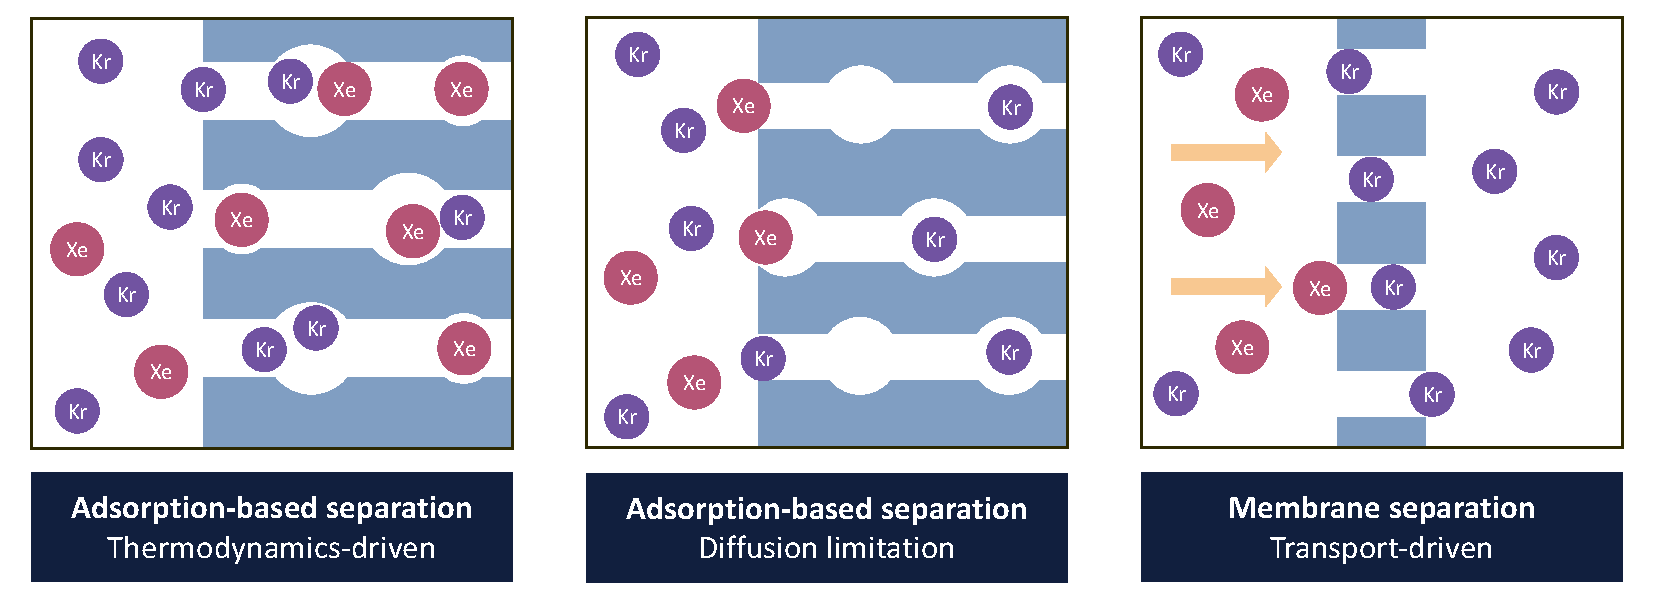
\includegraphics[width=0.95\textwidth]{figures/5-diffusion/Diffusion.pdf}
    \caption{Illustration of the comparative role of the thermodynamic and transport properties for Xe/Kr separation in nanoporous materials. From the transport dominated process of membrane separation to the thermodynamically equilibrated separation processes in the nanopores, different more nuanced cases could emerge where the diffusion imposes kinetic limitations.}\label{fgr:intro_diffusion}
\end{figure}

\section{Modeling the diffusion process}

% From the macroscopic brownian motion modeled by the
% Fick's law
Since the observation of pollen motion by the botanist Brown in 1826, the seemingly erratic movement of particles in a static bulk medium has been thoroughly observed and studied by scientists. Subsequently, Fick proposed a macroscopic model for this phenomenon, known as Brownian motion, by introducing the coefficient $D_x$ in a diffusion equation~\ref{eq:fick} (1D) based on experimental measurements of concentration $\phi$.\autocite{Fick_1855}. According to this law (valid only for independent particles), particles tend to move from regions of higher concentration to regions of lower concentration within the bulk medium.

\begin{equation}\label{eq:fick}
  \frac{\partial \phi}{\partial t} = D_x \frac{\partial^2 \phi}{{\partial x}^2}
\end{equation}

To gain a better understanding of the Brownian motion of suspended particles in a liquid, Einstein derived a microscopic model of diffusion motion based on the molecular-kinetic theory of heat in the momentous year of 1905.\autocite{einstein1905motion} To determine the self-diffusion coefficient (referred to as the ``diffusion coefficient'' hereafter), he observed the motion of an individual particle assumed to be independent of other particles, with time steps large enough to consider two consecutive motions as mutually independent. By considering the particle distribution of $N$ independent diffusing particles, he redefined the diffusion coefficient as a function of the mean squared displacement (MSD) of a particle. In tridimensional space, the following Einstein relation is applicable:
\begin{equation}\label{eq:einstein}
  \langle {r(t)}^2 \rangle = 2dD\e{diff}t = 6D\e{diff}t
\end{equation}
where  $d$ is the dimension of the space in which the particle diffuses ($d=3$ in a volume) and $r(t)$ is the displacement of a particle from the time $0$ to $t$. The brackets represent the average over all independent trajectories (different particles and different time origins). This equation can be generalized to the diffusion of an adsorbate in the adsorbed phase, which describes the ease of particle movement within a nanoporous material. A low diffusion coefficient indicates limited access to the structure's pores, as illustrated in Figure~\ref{fgr:intro_diffusion}. It is worth mentioning that in porous media, non-Fickian diffusion processes can occur, the MSD has a linear relation to time. For example, when particles are confined in a one-dimensional channel that does not allow a particle to jump over another, the dynamics is described by a single file diffusion equation, and the MSD has square root relation to time.\autocite{Levitt_1973}

To model the diffusion coefficient of xenon and krypton inside nanoporous materials, molecular simulations of the adsorbate displacements will be utilized. Although alternative approaches such as the Green-Kubo equation exist, the comparatively less complex Einstein law is preferred for self-diffusion calculations, as demonstrated by this cited comparative study~\cite{Maginn_2020}. This section will focus on various simulation techniques that can be used for evaluating diffusion in high-throughput screenings. Different methods of assessing the MSD of diffusing particles will be presented, starting from the straightforward approach of molecular dynamics to faster methodologies more suitable for screenings, such as machine-learned surrogate models and kinetic Monte Carlo simulations.

\subsection{Molecular dynamics}

Molecular dynamics (MD) simulations are used to reproduce the microscopic motion of molecules in a given system and to calculate thermodynamic averages by assuming the equivalence between time averaging and ensemble averaging (ergodic hypothesis). For other applications, mechanical properties, thermodynamic properties, or chemical properties can also be determined. However, the main focus here is on calculating diffusion coefficients of monoatomic molecules, with the discussion centered around averaging trajectories to obtain MSD values.

\subsubsection{Simulation details}

Molecular dynamics aims at describing the motion of particles, subjected to forces exerted by surrounding particles. This process can be viewed as a step-by-step integration of the Newton's law of motion. A particle $i$ of position $\mathbf{r}_i$ and mass $m_i$ subjected to a force $\mathbf{F}_i$ resulting from the cumulated interactions with its surroundings is accelerated according to this equation:
\begin{equation}\label{eq:newton}
  m_i\frac{\dd^2 \mathbf{r}_i}{{\dd t}^2} = \mathbf{F}_i
\end{equation}

In classical modeling, forces are determined using the aptly named forcefield that was previously introduced in Chapter 2.  In that context, intermolecular interactions were simplistically modeled by the Lennard-Jones (LJ) interaction potential between atom pairs, which is also employed in this section (although other methods for defining a forcefield exist). By utilizing the LJ potentials $U\ex{LJ}$ (defined in equation~\ref{eq:LJ}), the vectorial force $\mathbf{f}_{ij}$ between two atoms $i$ and $j$ can be derived:
\begin{equation}
  \mathbf{f}_{ij} = - \left.{\dfrac{\dd U\ex{LJ}_{ij}}{\dd r}}\right\rvert_{r=r_{ij}} \frac{\mathbf{r}_{ij}}{r_{ij}} = 24\epsilon_{ij}  \left(2{\left(\dfrac{\sigma_{ij}}{r_{ij}}\right)}^{12} - {\left(\dfrac{\sigma_{ij}}{r_{ij}}\right)}^{6}\right) \frac{\mathbf{r}_{ij}}{r_{ij}^2}
\end{equation}
where $\epsilon_{ij}$ and $\sigma_{ij}$ are the LJ parameters of the atom pair $ij$. The resulting force is obtained by summing the forces $\mathbf{F}_i=\sum_{j}\mathbf{f}_{ij}$ exerted by the surrounding atoms $j$. To reduce the computation time required, molecular simulations consider only the atoms within a specified cutoff radius.

Now that the force $\mathbf{F}_i$ has been defined, the molecule can be set in motion by numerically integrating equation~\ref{eq:newton} from time $t$ to time $t+\delta t$. Various methods exist to integrate equations of motion, such as the Euler or velocity-Verlet scheme presented in the book by Frenkel et al.\autocite{frenkel2001md} In this work, the focus will be on the \emph{leap frog} integration implemented in the RASPA2\autocite{dubbeldam2016} software used for the MD simulations. The position $\mathbf{r}_i$ and velocity $\dot{\mathbf{r}}_i$ are updated at each time step $\delta t$ using the following equations:
\begin{equation}\label{eq:frogleap_integration}
  \begin{split}
    \dot{\mathbf{r}}_i\left(t+\tfrac{1}{2}\delta t\right) & = \dot{\mathbf{r}}_i\left(t-\tfrac{1}{2}\delta t\right) + \tfrac{1}{m_i}\mathbf{f}_i \\
    \mathbf{r}_i\left(t+\delta t\right) & = \mathbf{r}_i\left(t\right) + \dot{\mathbf{r}}_i\left(t+\tfrac{1}{2}\delta t\right)\delta t
  \end{split}
\end{equation}
From the initial conditions $(\mathbf{r}_i(0),\dot{\mathbf{r}}_i(0.5\delta t))$, the center of mass of molecule $i$ can be translated to any position $\mathbf{r}_i(t_n=n*\delta t)$. The rotation step required for polyatomic molecules will be omitted since the study focuses solely on monoatomic noble gases. The different positions ${\left\{\left(t_n,\mathbf{r}_i(t_n)\right)\right\}}_{n=0,\ldots,N\e{tot}}$ constitute the total trajectory of the MD simulation (velocities are not mentioned for readability, but they are also propagated). This total trajectory can be used to derive the average MSD, which can be further analyzed to calculate the diffusion coefficient.

\subsubsection{Diffusivity calculation using an MD trajectory}

The MSD sampling technique implemented in RASPA2\autocite{dubbeldam2016}, presented in an article~\cite{Dubbeldam_2009} by several authors of the adsorption simulation software, was employed. The approach is based on a modified version of the order-$\mathbf{n}$ algorithm described in the book~\cite{frenkel2001msd} by Frenkel and Smit. The focus in this chapter will be on the multiple-window algorithm used to calculate the diffusion coefficients of xenon and krypton.

To understand this computation, it is necessary to first explain what the window algorithm does and how it can be generalized to the multiple-window algorithm. First, consider a single MD trajectory of duration $t\e{tot}=N\e{tot}\delta t$. This trajectory can be used to generate displacement of any size $\tau$. A straightforward approach would be to compute the square displacement ${\lVert\mathbf{r}_i(\tau)-\mathbf{r}_i(0)\rVert}^2$ for a sub-trajectory $\mathcal{T}(0\rightarrow\tau)$ of duration $\tau$. However, this alone is insufficient to obtain a statistically meaningful average of the MSD, as described by the Einstein equation~\ref{eq:einstein}. By assuming independence between two movements of the same particle separated by a time $\delta t$, as hypothesized in Einstein's paper~\cite{einstein1905motion}, shifting the origin of time by $\delta t$ would yield another trajectory. This process can be repeated $i$ times while $\tau + i\delta t\leq t\e{tot}$. Although highly accurate, this approach is highly inefficient when $\tau \gg \delta t$ since two consecutive sub-trajectories $\mathcal{T}(i\delta t\rightarrow\tau+i\delta t)$ and $\mathcal{T}((i+1)\delta t\rightarrow\tau+(i+1)\delta t)$ would be very similar. 

To efficiently sample the trajectory into independent sub-trajectories, a sampling time step of $\delta \tau\lesssim\tau$, on the same order of magnitude as $\tau$, can be employed. To achieve this, the window approach first defines a value $\delta \tau$ and generates $N_{\tau} = \lfloor(t\e{t ot} -\tau)/ \delta\tau \rfloor$ different sub-trajectories $\left\{\mathcal{T}(0\rightarrow\tau), \mathcal{T}(\delta\tau\rightarrow\tau + \delta\tau), \ldots, \mathcal{T}(N_{\tau}\delta\tau\rightarrow\tau + N_{\tau}\delta\tau)\right\}$ of duration $\tau=k\delta\tau$, where $k$ is an integer ranging from $1$ to $K$ that defines the time window to be sampled. This allows the calculation of the MSD $\langle {r(\tau)}^2 \rangle$ for duration values of $\tau$ equal to $\delta\tau, \ldots, K\delta\tau$. The resulting MSD $\langle {r(\tau)}^2 \rangle$ is linear with respect to time, it can then be fitted to equation~\ref{eq:einstein} to obtain the diffusion coefficient. The trajectory generation using the window approach is illustrated in Figure~\ref{fgr:window_msd} for a decomposition into sub-trajectories of a duration $\tau=3\delta\tau$ shifted by $\delta\tau$.

\begin{figure}[ht]
  \centering
    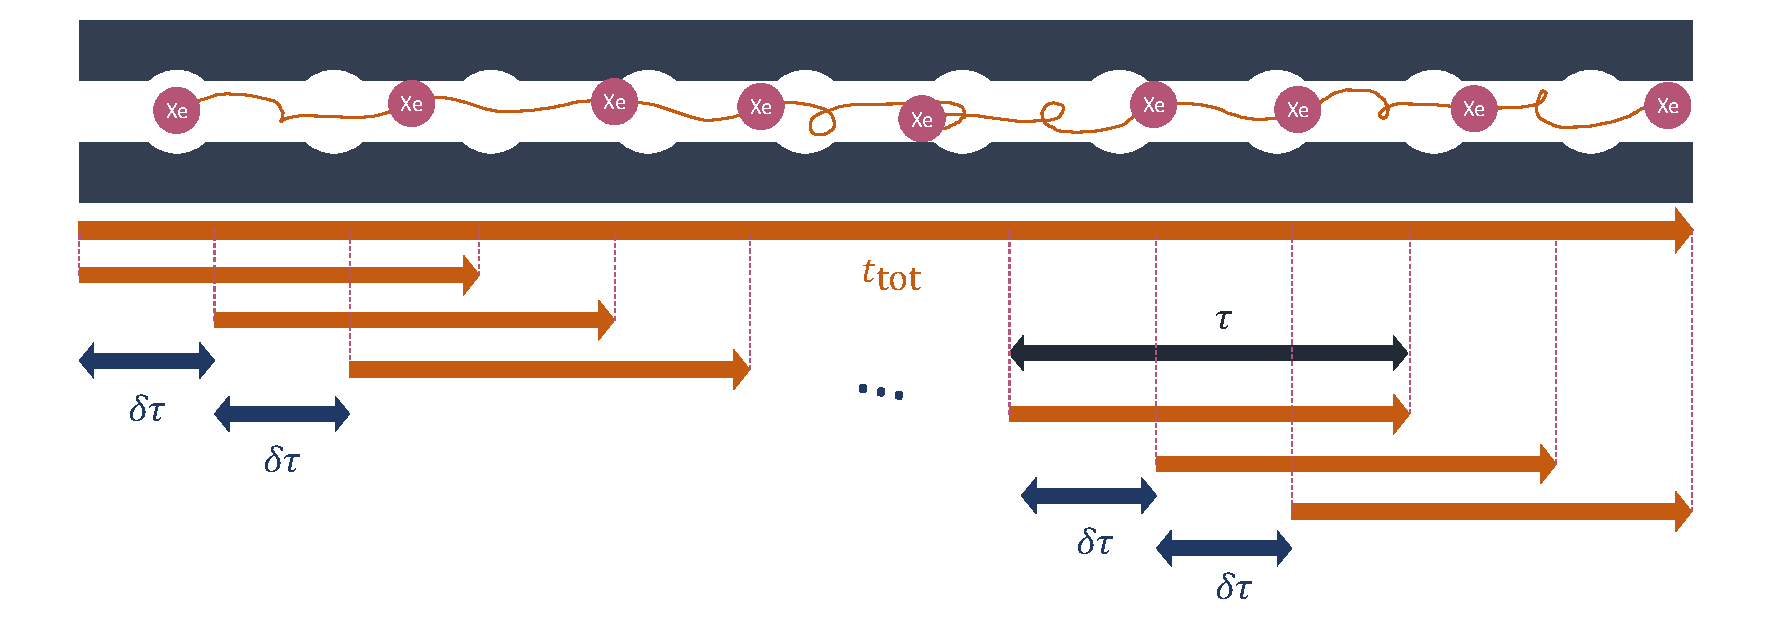
\includegraphics[width=0.95\textwidth]{figures/5-diffusion/diffusion_averaging.pdf}
    \caption{Illustration of the generation of trajectories of size $\tau$ by shifting the origins of multiple durations $\delta\tau$. }\label{fgr:window_msd}
\end{figure}

The major drawback of this method is that a timescale $\left\{\delta\tau, \ldots, K\delta\tau\right\}$ needs to be defined in advance. To access the different timescales within a single simulation, the multiple-window algorithm developed by Dubbeldam et al.\ and implemented in the RASPA2 software for calculating mean squared displacements (MSD) in molecular dynamics simulations is employed.

The different time windows are recursively defined using the default parameters of RASPA2. The first time window is defined by $K=25$ displacements with durations $\delta t, 2\delta t, \ldots,(K-1)\delta t$ and a shift of $\delta t$ (the default shift value $\delta t$ of the first window can be modified using the parameter ``SampleMSDEvery''). The second window is then based on a sampling time $\delta \tau_1 = K\delta t$, and the sub-trajectories have durations $\tau_1^{(1)} = \delta\tau_1,\ldots,\tau_1^{(K-1)} = (K-1)\delta\tau_1$. This recursive process is repeated, where the $i$\e{th} window has a sampling time of $\delta \tau_i = K^i\delta t$ and sub-trajectories with durations $\tau_i^{(1)} = \delta\tau_i,\ldots,\tau_i^{(K-1)} = (K-1)\delta\tau_i$. A window algorithm similar to the one described above is applied to each window. The algorithm terminates when no further window can be generated, i.e., when $\tau_n^{(k)}>t\e{tot}$ where $n$ is the index of the window and $k$ is the index in the single-window algorithm that defines the desired sampling time with respect to $\delta\tau_i$. The timescale $\delta \tau_i = K^i\delta t$ sampled follows a geometric progression, allowing access to very different timescales. This enables the identification of the timescale corresponding to the diffusion regime (linear relationship between the MSD and the duration of the sub-trajectories used in the averaging). The different timescales and the exponent value $b$ from fitting a function of the form $x \mapsto ax^b$ for the different time windows are illustrated in the next section (Figure~\ref{fgr:MSD_init}) --- values of $b$ close to $1$ can be associated with a diffusion regime. The determination of the diffusion coefficient is then simplified to a simple fitting problem, which will be further explained in the presentation of the diffusion coefficient screening in section~\ref{sct:md_screening}.

This methodology can then be replicated to thousands of structures to characterize the diffusion properties of these materials. Numerous screenings have already been conducted in the literature, as presented in Chapter 1, specifically in the section dedicated to transport property. The prediction of these quantities using machine learning will now be explored in more detail.

\subsubsection{ML modeling}

In a very recent study, Daglar et al.\ used an ML model to predict the diffusion coefficient of 100,000 hypothetical MOFs by utilizing data on around 5,000 CoRE MOF structures.\autocite{Daglar_2022} Alongside conventional geometrical descriptors, they employed chemical composition descriptors and the heat of adsorption as the input features of their machine learning model to predict the diffusion coefficients of \ce{H2}, \ce{CH4}, \ce{N2} and \ce{He} within various MOF materials from CoRE MOF 2019 (training dataset) and hMOF (testing dataset). The combination of kinetic and thermodynamic data for the characterization of MOF materials is an intriguing approach. However, a key limitation of most existing approaches in the literature is the lack of structure--property relationship that elucidates the underlying microscopic origins of diffusion coefficient values.

Following a similar approach to the thermodynamic screening (Chapters~2--4), the present work on transport property screening aims to establish structure-property relationships between diffusion coefficients and geometric descriptors of MOF structures. To gain deeper insights into the diffusion process, the diffusion activation energy will be evaluated using energy grid-based methods described in the literature. These techniques are designed to enhance the prediction of diffusion coefficients, either through direct calculations or by employing ML surrogate models. To this end, kinetic Monte Carlo approach will be introduced, which, although less accurate than the MD approach, offers significantly higher computational efficiency.

\subsection{Lattice kinetic Monte Carlo}

The lattice kinetic Monte Carlo method relies on a predefined lattice of stable points corresponding to adsorption sites. Each site is connected to another if there exists a diffusion path (narrow channel) between them. To calculate the probability of transition from one site to another, a transition state (TS) within the narrow channel corresponding to the highest energy point along the minimal energy diffusion path (the saddle point), must be defined. In the transition state therory, the transition probability is defined based on the energy barrier that must be overcome to traverse the channel. Once the lattice is established, the adsorbate can be propagated from one site to another using the different transition probabilities. Although this approach yields a coarse-grained trajectory compared to the one obtained through MD simulations, it is sufficient for computing the MSD and the diffusion coefficient.


\begin{figure}[ht]
  \centering
    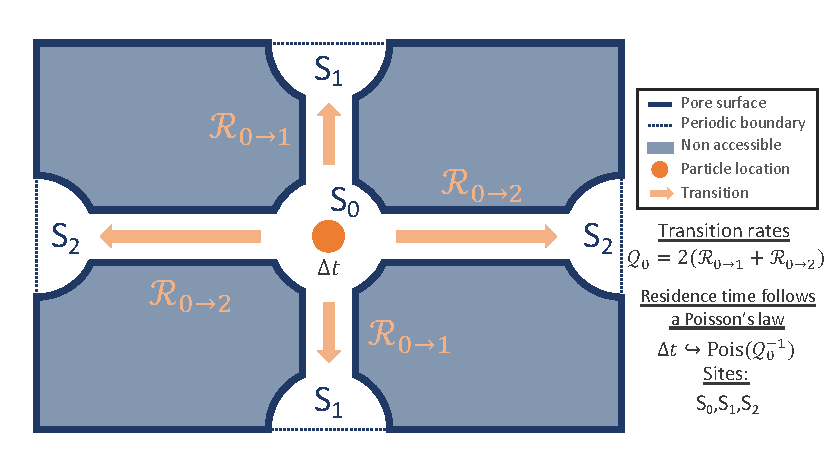
\includegraphics[width=0.8\textwidth,trim={0.2cm 0.2cm 0cm 0.7cm},clip]{figures/5-diffusion/kinetic_MC.pdf}
    \caption{Illustration of the core principle of lattice kinetic Monte Carlo in a periodic system. Within the periodic system, the movement of particles is governed by transition probabilities from one site to another. The transition rates are determined using the activation energy needed to move to the transition state between the two stable adsorption sites, as shown in equations~\ref{eq:trans_rate_path} and~\ref{eq:trans_rate}. }\label{fgr:kMC_principle}
\end{figure}

\subsubsection{Transition state theory for diffusion}

In chemistry, the kinetics of a reaction are often explained using transition state theory. This theory compares the energy of the reactants to that of the transition state, allowing for the calculation of the reaction rate. Along a reaction path, this rate is proportional to the ratio between the Boltzmann factor at the transition state and the integration of Boltzmann factors along the reaction path.

This definition can be directly transposed to the case of a diffusion path instead of a reaction path. Thus, the diffusion rate $\mathcal{R}_{0\rightarrow 1}$ from site $0$ to $1$ can be defined as follows:
\begin{equation}\label{eq:trans_rate_path}
  \mathcal{R}_{0\rightarrow 1} = \kappa\sqrt{\frac{k\e{B}T}{2\pi m}}\frac{e^{-\beta E(\mathbf{r}\ex{TS})/k\e{B}T}}{\int\e{path}e^{-\beta E(\mathbf{r})/k\e{B}T}\dd\mathbf{r}}
\end{equation}
$\kappa$ is the Bennet-Chandler dynamic correction factor (or recrossing probability),\autocite{BENNETT1977} and $\kappa=\tfrac{1}{2}$ if it is equiprobable to reach both sites from the transition state. This requires the determination of the optimal diffusion path before determining the diffusion rate. Wang et al. (2022) adopted this approach in their noble gas separation screening, where they first determined the minimal energy path before calculating diffusion rates.\autocite{Wang_2022}

Another approach involves determining a transition surface through which the adsorbate passes to diffuse along the channel of the material. In this case, only the determination of the transition only, but it relies on another definition of the transition rate $\mathcal{R}_{0\rightarrow 1}$:
\begin{equation}\label{eq:trans_rate}
  \mathcal{R}_{0\rightarrow 1} = \kappa\sqrt{\frac{k\e{B}T}{2\pi m}}\frac{\int_{\mathcal{S}(TS)}e^{-\beta E(\mathbf{r})/k\e{B}T}\dd\mathbf{r}}{\int_{\mathcal{V}(\text{S}_0)}e^{-\beta E(\mathbf{r})/k\e{B}T}\dd\mathbf{r}}
\end{equation}
where the integration for the transition state is performed on a bottleneck surface that a diffusing particle must cross to move from the volume occupied by site $0$ to the one occupied by site $1$.

\subsubsection{TuTraST algorithm for kinetic MC}\label{sct:tutrast}

In this section, the focus shifts to the second approach, which relies on the determination of a transition state as a surface. This approach was developed by Mace et al.\autocite{Mace_2019}\ and involves detecting merging points between basins that represent the adsorption sites. The algorithm developed for this purpose is known as TuTraST,  which stands for Tunnels and Transition States. It is a search algorithm that aims to identify the tunnels and transition states that separate different adsorption ``basins'' within them. Once the adsorption sites, transition states, and connecting tunnels are identified, hopping rates between stable adsorption sites can be calculated using Equation~\ref{eq:trans_rate}. Finally, a lattice kinetic Monte Carlo simulation can be employed to move particles within a simplified hopping diffusion system to determine the MSD and, ultimately, the diffusion coefficient.

\begin{figure}[ht]
  \centering
    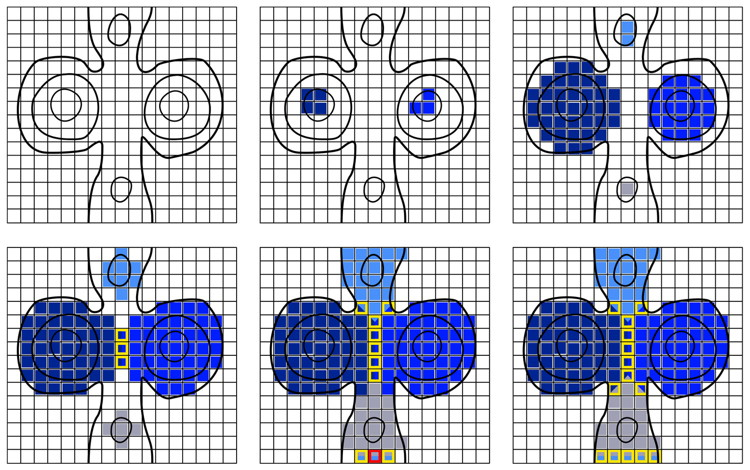
\includegraphics[width=0.6\textwidth]{figures/5-diffusion/tutrast.jpg}
    \caption{ Illustration of the cluster growth and the identification of boundary points in the TuTraST algorithm\autocite{Mace_2019}. The clusters are grown from left to right and top to bottom. A tunnel is detected when the points are connected all the way from one periodic boundary to another (red). The boundary points assigned to the TS surface are indicated in yellow. Reprinted with permission from the original paper~\cite{Mace_2019} copyright \copyright\ 2019 American Chemical Society. }\label{fgr:tutrast}
\end{figure}

In practice, the calculation of an energy grid that detects all the different components of the lattice is required. The algorithm iterates over different energy values from $E\e{min}+\delta E, \ldots, E\e{min}+N\delta E$, such that the maximum energy is below a predetermined energy cutoff $E\e{min}+N\delta E<E\e{cutoff}$. At the initial step, the clusters of grid points with an energy below $E\e{min}+\delta E$ are naturally formed based on their connectivity. Then, at iteration level $L$, the clusters found in the previous iteration $L-1$ are grown layer by layer (one layer corresponds to the immediate neighbors on the grid), as shown in Figure~\ref{fgr:tutrast}. If a layer touches another cluster, a boundary point is identified --- it is tagged as a point of the TS surface if the energy barrier to go from the basin to this point is sufficiently high, else the energy barrier is negligible, and the basins are merged. At the end of the process, the boundary values are clustered and assigned as the transition surface between different pairs of adsorption basins. If the points of the basins and boundary surfaces are connected all the way through, a tunnel can be defined for diffusion to occur. After a sufficient number of iterations, tunnels with different basins separated by transition state surfaces are established. A kinetic Monte Carlo simulation can then be performed to determine the diffusion coefficient within each tunnel. The diffusion coefficient in the material corresponds to a weighted average of the diffusion coefficients in each tunnel, with the weight determined by the probability of presence in each tunnel, which corresponds to the sum of the Boltzmann factors (proportional to the Henry coefficient in a given tunnel).

This approach is very promising as it is significantly more efficient than MD simulation-based techniques. The code of Mace et al.\autocite{Mace_2019} implemented in Matlab (although not computationally very efficient) already outperforms most MD simulations in terms of computation time for diffusion coefficient calculation, with minimal compromise in accuracy, as demonstrated in their diffusion coefficient screening of zeolites. To enhance efficiency further, the algorithm for efficient search of transition states was rewritten in C++. At this stage of development, the focus was on determining the diffusion activation energy, which is independent of transition state detection. Detailed algorithmic information for determining the diffusion activation energy in nanoporous materials using the in-house algorithm is provided in section~\ref{sct:algo_diff}, along with the projected development of a faster lattice kinetic Monte Carlo simulation inspired by the TuTraST algorithm.


\section{Self-diffusion screening}\label{sct:md_screening}

To complement the thermodynamic screenings conducted in chapters 2--4, a screening of transport properties, specifically diffusion coefficients, was also performed. This section presents the screening approach and analyzes the diffusion coefficients in comparison with typical geometric descriptors.

\subsection{Diffusion in a selective material}

Before delving into the details of the screening study, the approach adopted for calculating diffusion coefficients using MSD values is demonstrated through an example: SBMOF-1\autocite{Banerjee_2016}. This preliminary study aids in calibrating the time parameters (time step, maximum time) for the final screening study.

First, an MD simulation of 500 million steps (approximately 1--2 days of simulation) was conducted, including a thousand initialization steps and 100 thousand equilibration steps to model a xenon atom diffusing in the \texttt{KAXQIL}\autocite{Banerjee2012} MOF at ``infinite dilution''. To achieve infinite dilution, the box size was adjusted to prevent interactions between different adsorbates. In these conditions, as shown in Figure~\ref{fgr:MSD_init}, there are different timescales at which distinct transport phenomena occur. 

Within the range of \SI{1}{\fs} to \SI{1}{\ps}, a ballistic regime is observed, with the mean squared displacement following a squared dependence. For a particle of mass $m$, the MSD $\langle {r(\tau)}^2 \rangle$ in this regime obeys a simple ballistic relation (length equals velocity multiplied by time):
\begin{equation}
  \langle {r(\tau)}^2 \rangle = v_m^2 \tau^2 = \frac{k\e{B}T}{2\pi m}\tau^2
\end{equation}
where $v_m$ is the average velocity of a particle, following the Maxwell-Boltzmann distribution at temperature $T$. Calculating the squared mean velocity $v_m^2$ using the standard Maxwell-Boltzmann relation yields a value of \SI{3}{\square\m\per\square\second}, which closely matches the value of \SI{2.8}{\square\m\per\square\second} obtained by the fit in the right plot of Figure~\ref{fgr:MSD_init}. This initial regime corresponds to the movement of particles subjected to thermal agitation, but it holds little significance for diffusion.

\begin{figure}[ht]
  \centering
    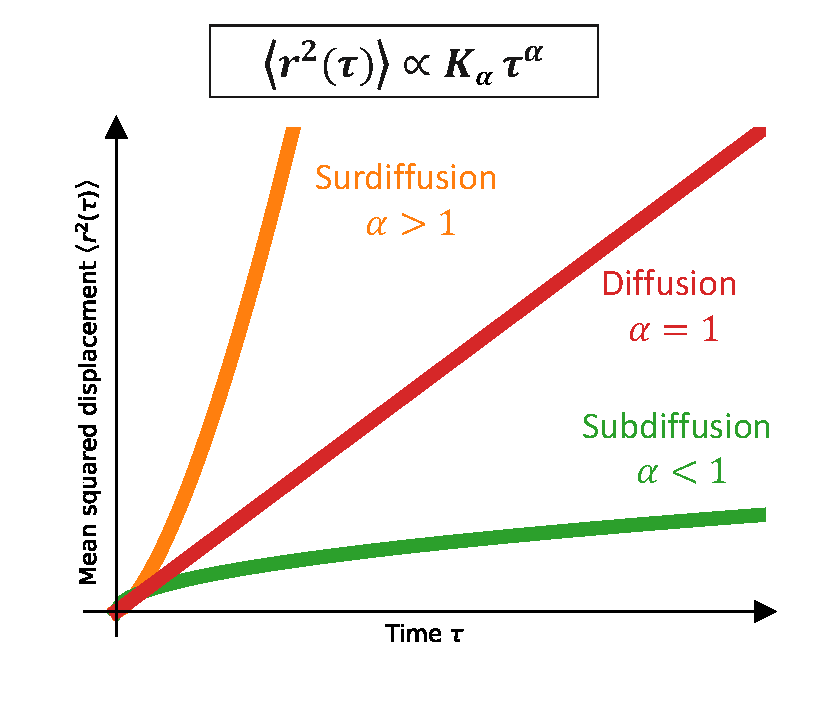
\includegraphics[width=0.48\textwidth]{figures/5-diffusion/MSD_anomalous_diffusion.pdf}
    \includegraphics[width=0.48\textwidth]{figures/5-diffusion/MSD_Xe_KAXQIL_clean.pdf}
    \caption{Left: Different regimes that could be observed in an MSD plot as a function of time. The ballistic regime can be considered super-diffusional, while the normal diffusion follows a linear relation described by the Einstein equation~\ref{eq:einstein}. The sub-diffusion regime commonly occurs in obstructed media such as nanoporous materials. The different regimes can be observed in the right plot of the actual MSD, which is calculated using the multiple-window method. Fittings are performed using a generic function $K_\alpha\tau^\alpha$, and the exponents $\alpha$ are provided in the legend. }\label{fgr:MSD_init}
\end{figure}

A transition from the ballistic regime to the pseudo-diffusional regime (where the exponent has not yet reached 1) is observed in the plot in cyan. Between \SI{1}{\ps} and \SI{100}{\ps}, a sub-diffusion regime is observed, characterized by an MSD that follows a power function of time, $\langle {r(\tau)}^2 \rangle=K_\alpha\tau^\alpha$, with an exponent less than $1$, as illustrated in the left plot of Figure~\ref{fgr:MSD_init}. This regime corresponds to the confinement of xenon particles within adsorption pores, where only thermal vibration occurs, and no diffusion hopping is observed at this timescale. Diffusion appears to begin at the \SI{10}{\ns} timescale. The MSD between \SI{0.01}{\ns} and \SI{0.4}{\ns}, as shown in Figure~\ref{fgr:MSD_linear_init}, represents a sub-diffusional regime due to the confinement imposed by the nanopores of \texttt{KAXQIL}. However, at \SI{0.4}{\ns}--\SI{9}{\ns}, the MSD starts to exhibit an exponent of $0.7$, which is closer to $1$, allowing for a linear fit, albeit imperfect (Figure~\ref{fgr:MSD_linear_init}). Ideally, trajectory sampling on the order of tens of nanoseconds would be desirable for the next timescale. However, with an MD time step of \SI{1}{\fs}, this would multiply the computation time by at least 5 (1--2 weeks for one MD simulation), which becomes prohibitive.

\begin{figure}[ht]
  \centering
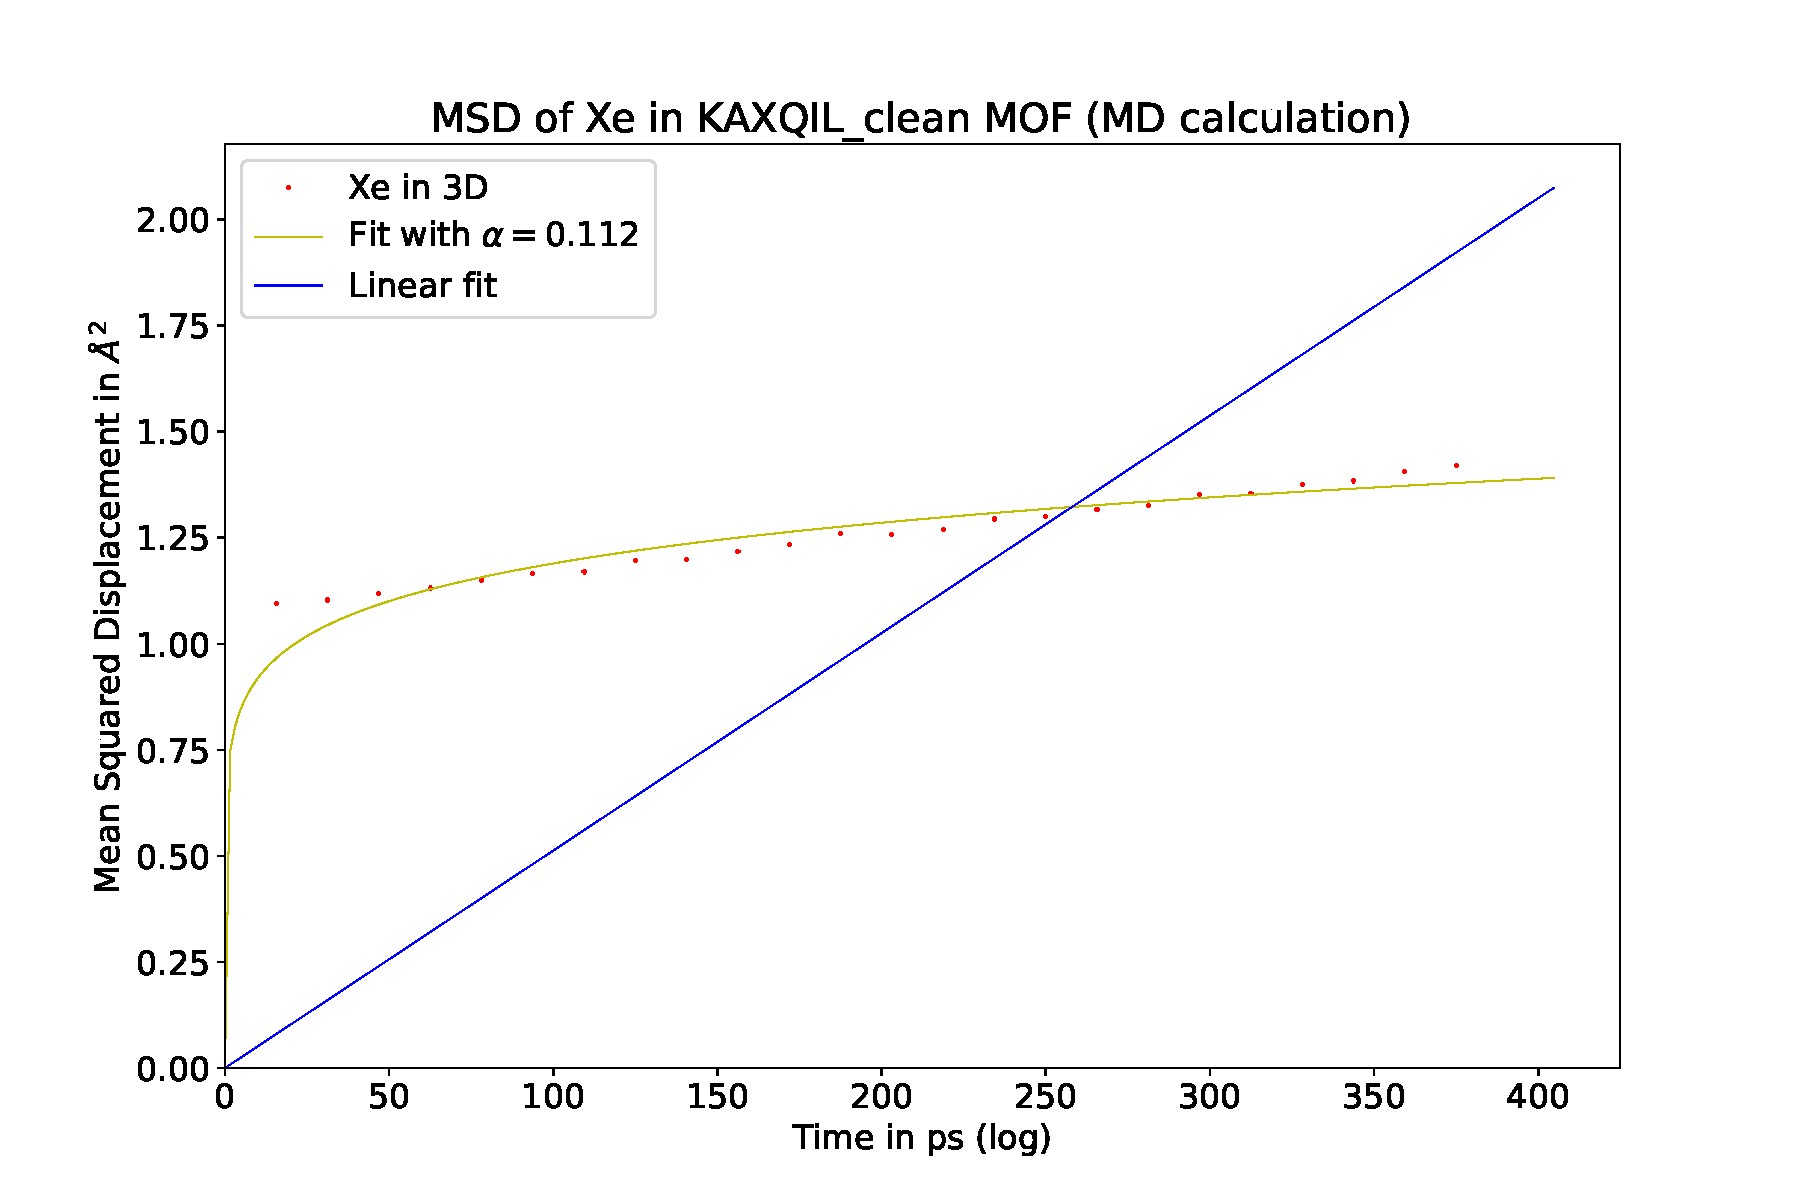
\includegraphics[width=0.48\textwidth]{figures/5-diffusion/MSD_Xe_coeff_KAXQIL_clean_1.pdf}
\includegraphics[width=0.48\textwidth]{figures/5-diffusion/MSD_Xe_coeff_KAXQIL_clean_2.pdf}
\caption{ Plots of the MSD at the last two timescales considered in Figure~\ref{fgr:MSD_init}. On the left, the timescale between \SI{0.01}{\ns} and \SI{0.4}{\ns} is considered. The MSD is fitted using a power function with the same previously determined exponent, and a linear fit is provided to demonstrate its incompatibility with the diffusion equation. On the right, a similar approach is employed for the timescale between \SI{0.4}{\ns} and \SI{9}{\ns}. }\label{fgr:MSD_linear_init}
\end{figure}

By fitting a linear relation using the right plot of Figure~\ref{fgr:MSD_linear_init} and deducing the diffusion coefficient, an underestimated value of the diffusion coefficient of $2.24\times 10^{-8}$~\si{\square\cm\per\s} is obtained --- it is an underestimation due to the concave nature of the MSD, which reduces the slope in the fitting process. However, this value is already a good estimation of the diffusion coefficient, considering the relatively high value of the exponent $\alpha=0.7$ in the fitting equation $K_\alpha\tau^\alpha$.

To account for the randomness in the initial position of xenon (block pockets have been calculated for a \SI{1.5}{\angstrom}-radius probe), it is necessary to measure the effect of running different MD simulations of the value of the diffusion coefficients. The uncertainty across various MD simulations with different initial positions determined by different random seeds needs to be quantified. In RASPA2, the random seed is equal to the UNIX time upon launching the MD simulation, ensuring that each of the $10$ different MD simulations is assigned a different random seed while using the exact same parameters, as previously mentioned. The diffusion coefficient values were averaged over these simulations, resulting in an average diffusion coefficient of $2.13\times 10^{-8}$~\si{\square\cm\per\s} and a standard deviation of $0.37\times 10^{-8}$~\si{\square\cm\per\s}, representing approximately {17\%} of the average value. The uncertainty in the diffusion coefficient is estimated to be around {17\%} for a relatively low coefficient of around $10^{-8}$ cm²/s, with lower uncertainty expected for less obstructive materials. It is worth mentioning that in the particular case of \texttt{KAXQIL}, where all pores are symmetrically equivalent, the dynamics is more straightforward than for more complex pore architectures that will be tackled later in this chapter.

Increased confidence in the method led to the exploration of higher timescales beyond the reach the previous MD simulation, as the occurrence of the diffusion regime was observed at the \SI{10}{\ns} timescale. \todo{1 fs and 2.5 billion steps, results to compare} An initial calculation with 500 million steps and a timestep of \SI{5}{\fs} was performed to validate the diffusion coefficient value. The time window between \SI{2}{\ns} and \SI{47}{\ns} was considered, and the MSD was calculated from approximately 200 sampled trajectories, resulting in reasonably accurate values. A more accurate diffusion coefficient of $2.6\times 10^{-8}$~\si{\square\cm\per\s}\todo{check the} was obtained, which is very close to the value obtained using the previous approach. The value is slightly higher (which was expected), as the previous value was overestimated. Thus, this approach is consistent with the previous one.

\begin{figure}[ht]
  \centering
  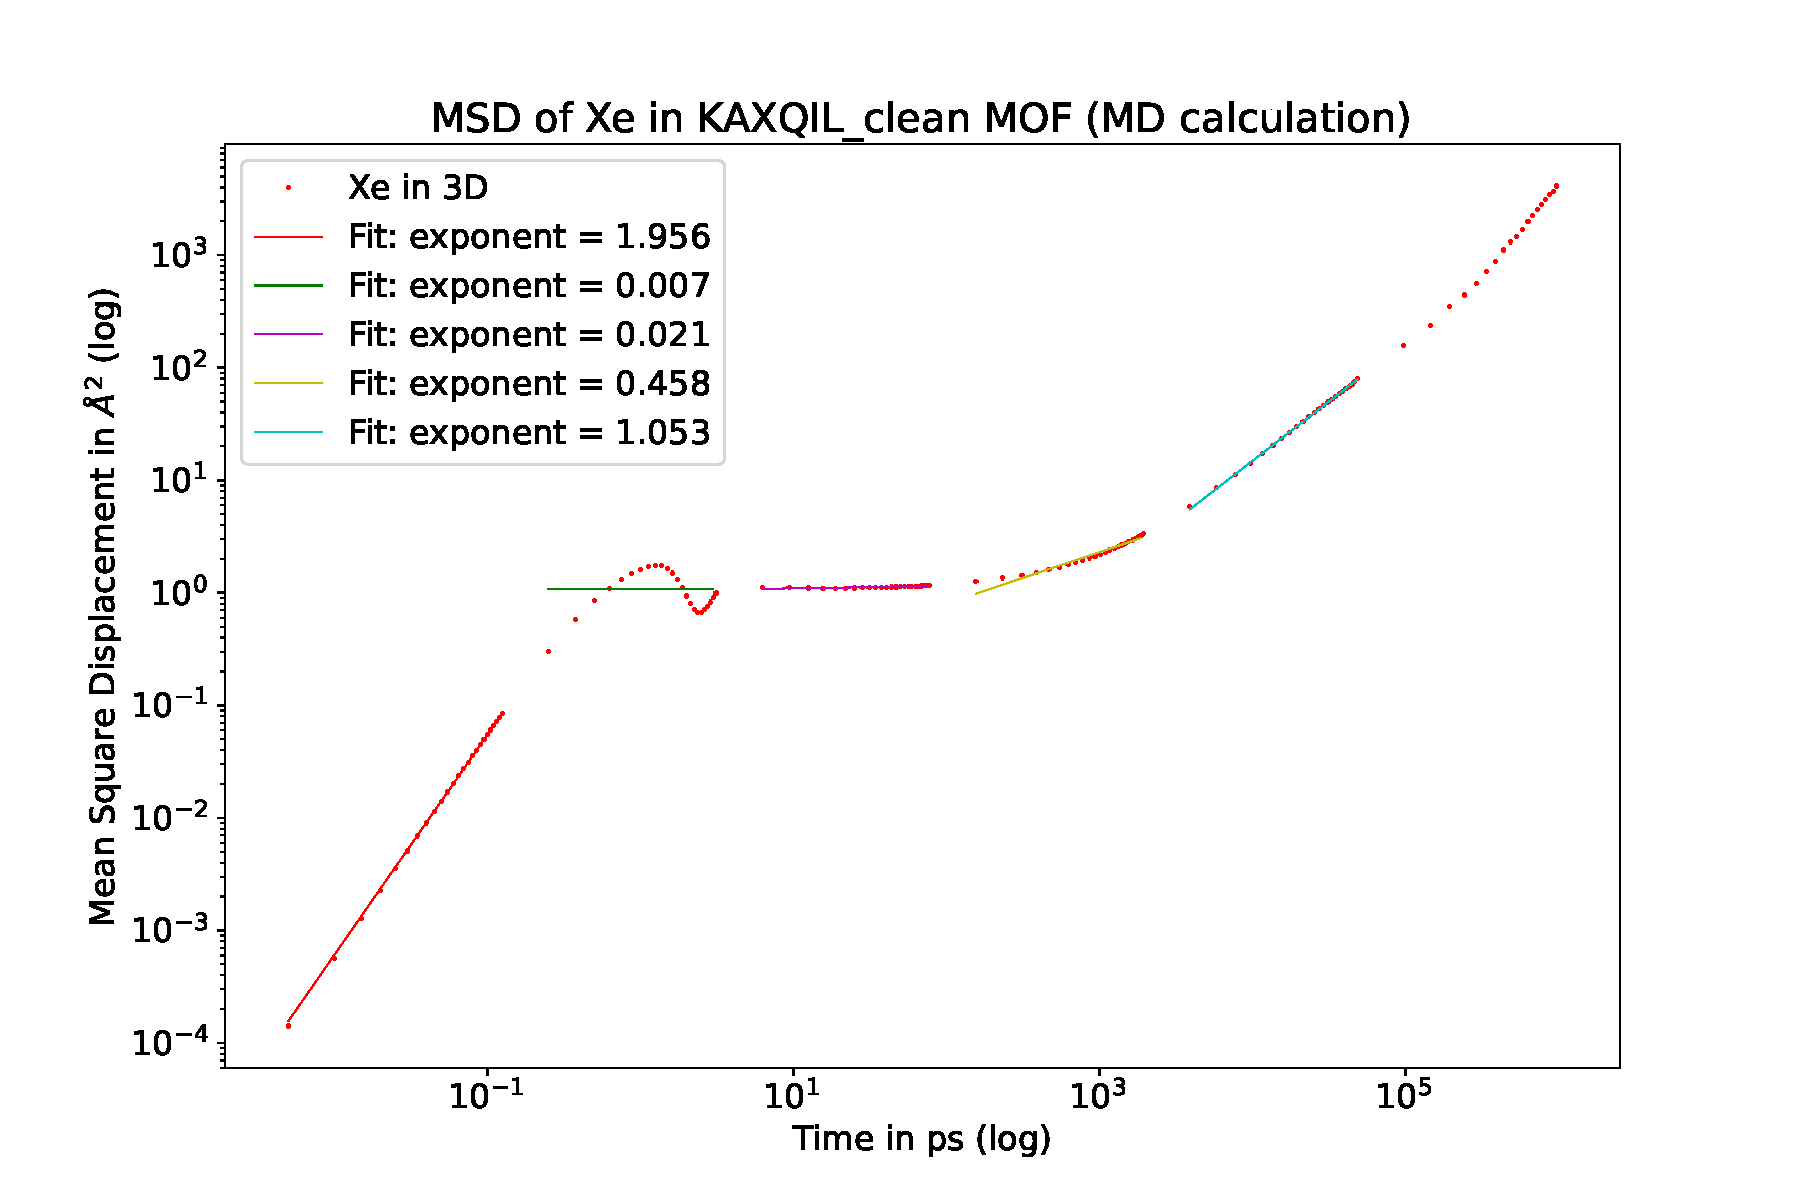
\includegraphics[width=0.48\textwidth]{figures/5-diffusion/MSD_Xe_KAXQIL_clean_5fs.pdf}
  \includegraphics[width=0.48\textwidth]{figures/5-diffusion/MSD_Xe_coeff_KAXQIL_clean_5fs.pdf}
\caption{ On the left panel, the MSD in log-log scale and a fit to the relation $\text{MSD}(\tau) = K_\alpha\tau^\alpha$ using an MD simulation of a \SI{5}{\fs}-time step and 500 million steps are shown. A better linear fit is obtained with this new configuration of the MD simulation compared to Figure~\ref{fgr:MSD_init}, as more timescales are explored while utilizing the same computational resources. On the right panel, the MSD on the timescale of the diffusion regime is presented. The linear fit demonstrates improved performance compared to the previous Figure~\ref{fgr:MSD_linear_init}.}\label{fgr:MSD_5fs}
\end{figure}

To further support the use of a higher time integration step, the origin of the value of \SI{1}{\fs} needs to be understood. This value is typically justified by the Nyquist-Shannon sampling theorem, which suggests that the integration step should be at most half of the period of the fastest vibration within the system. In the case of a C--H vibration, the maximum time step value is \SI{5}{\fs}, and to be on the safe side, a time step of $1$--$2$~\si{\fs} is chosen in most diffusion studies in nanoporous materials.\autocite{Bukowski_2021}. However, in the system of xenon diffusing in a rigid environment, there are no vibrational limitations as previously described. It is hypothesized in this thesis that using higher time steps in this situation can provide easier access to longer timescales. Nevertheless, further studies are required to ensure the validity of the quantities derived from these MD simulations. The value of \SI{5}{\fs} is at the higher end of what is typically observed in MD simulations, but it can be justified by the rigidity of the framework and the adsorbate being considered. Even higher time steps could be tested, but for more reliable results, a reasonable middle ground of \SI{5}{\fs} was chosen for all high-throughput screening of the transport properties.

\subsection{High-throughput screening of diffusion coefficients}

\subsubsection{Screening procedure}

To incorporate transport properties into the analysis, MD calculations were performed on 6,525 non-disordered, highly selective materials for xenon or krypton at infinite dilution (no guest--guest interactions). For each material, MD simulations were planned with 500 million steps using the RASPA2 script on the calculation machines (that are restricted to 24-hour runs). To let the simulation run a maximum of steps, 2 to 3 restarts were performed on the slowest simulations, such that every MSD data was obtained after 2--3 days. Out of the planned 500 million steps, only 432 structures \todo{Average number of timsteps completed} completed the simulations at the end of the process. However, this does not imply that the MSD data cannot be utilized for determining diffusion coefficients since the MSD are printed. In fact, 5,125 MSD data are exploitable even if the total 500 millions steps were only partially completed. 

To determine the diffusion coefficients, two timescales (2--47\si{\ns} and 50--950~\si{\ns}) were analyzed to fit the MSD with a linear function. The linear fit with the highest determination coefficient (within the range of $0$ to $1$) for both timescales was chosen to obtain a diffusion coefficient value. After this step, structures with a determination coefficient (R$^2$ that measures the correlation) below $0.9$ were removed, leaving 5,125 structures for drawing structure-diffusivity relationships --- these structures, for which there is a high degree of confidence in the diffusion coefficient values, will be comparatively studied against different geometrical and thermodynamic quantities in this section. Finally, the final 5,125 diffusion coefficients obtained correspond to the slopes of the best linear fit between the 2--47\si{\ns} and 50--950~\si{\ns} timescales.\todo{check FX}

This approach focuses exclusively on the linear relations between the MSD and time for determining self-diffusion at infinite dilution. The analysis does not explore the nature of the transport property (e.g., single-file diffusion\autocite{Lin_2005}), by comparing, for example, the exponent of the generalized formula $\text{MSD}(\tau) = K_\alpha\tau^\alpha$ with structural descriptors. The more complex diffusion at higher loading values, which may be more accurately described by a collective diffusion coefficient instead of the self-diffusion coefficient, is also not studied. The objective of this study is to identify materials that do not present kinetic limitations, as observed in the case of \texttt{KAXQIL}\autocite{Banerjee2012} (where the diffusion coefficient of xenon is approximately ten thousand times lower in the material than outside).

\subsubsection{Structure--diffusivity relationships}\label{sct:xenon_diff_screen}

In this section, different relationships between the diffusion coefficient and simple geometrical descriptors will be presented. A forcefield-dependent definition of radii was chosen to ensure better correlation with the results of the MD simulation that utilized the UFF forcefield. The geometrical descriptors were calculated using Zeo++ and these radii to determine the PLD, the largest sphere diameter D$_{if}$ along a free path, the surface area, and the pore volume, as explained in Chapter 2. The use of UFF-based radii for the PLD was further justified by the original paper~\cite{Hung_2021}, which demonstrated a stronger correlation between the PLD and the diffusion constant. This correlation can also be observed in Figure~\ref{fgr:diff_pld}. The PLD calculated using the standard CCDC-defined atom radii does not fit the diffusion coefficient as well as the UFF-defined PLD. As shown in a smaller scale in the article~\cite{Haldoupis_2010} (see Figure~\ref{fgr:Haldoupis_2010} in Chapter 1), there is a linear relationship between the diffusion activation energy (logarithmic transform of the diffusion coefficient) and the PLD. This linear relationship is much noisier for the PLD defined by the standard CCDC radii than for the UFF-based PLD.

Beyond the practical considerations regarding the calculation of geometrical descriptors, the PLD outlines the variation of diffusion performance within nanoporous materials. First, a linear relationship was observed, as previously highlighted, followed by a plateau. In the first zone, xenon is constrained by channels narrower than its kinetic radius. The diffusion coefficient rises with increasing channel width, and this positive correlation persists until the channel width exceeds approximately \SI{4.6}{\angstrom}. Beyond this threshold, the diffusion coefficient stabilizes around $3\times 10^{-4}$\si{\square\cm\per\s}. Variations in this plateau region can only be attributed to other phenomena, such as tortuosity within nanopores or the chemical nature of the surface of nanopores. The diffusion coefficient value can be interpreted as the diffusion coefficient of a ``free'' xenon, which is less influenced by the surrounding pore surface. For PLD values exceeding \SI{5}{\angstrom}, the channels are sufficiently wide to allow for xenon toonly undergo a minor slowdown. These findings are consistent with experimental data that measured the diffusion coefficient of xenon dissolved in water at different temperature conditions, where a value of $10^{-5}$~\si{\square\cm\per\s} at \SI{303}{\kelvin} was obtained \autocite{Wise1968}, aligning with the values observed centered around $3\times 10^{-4}$~\si{\square\cm\per\s} at the plateau.

\begin{figure}[ht]
  \centering
    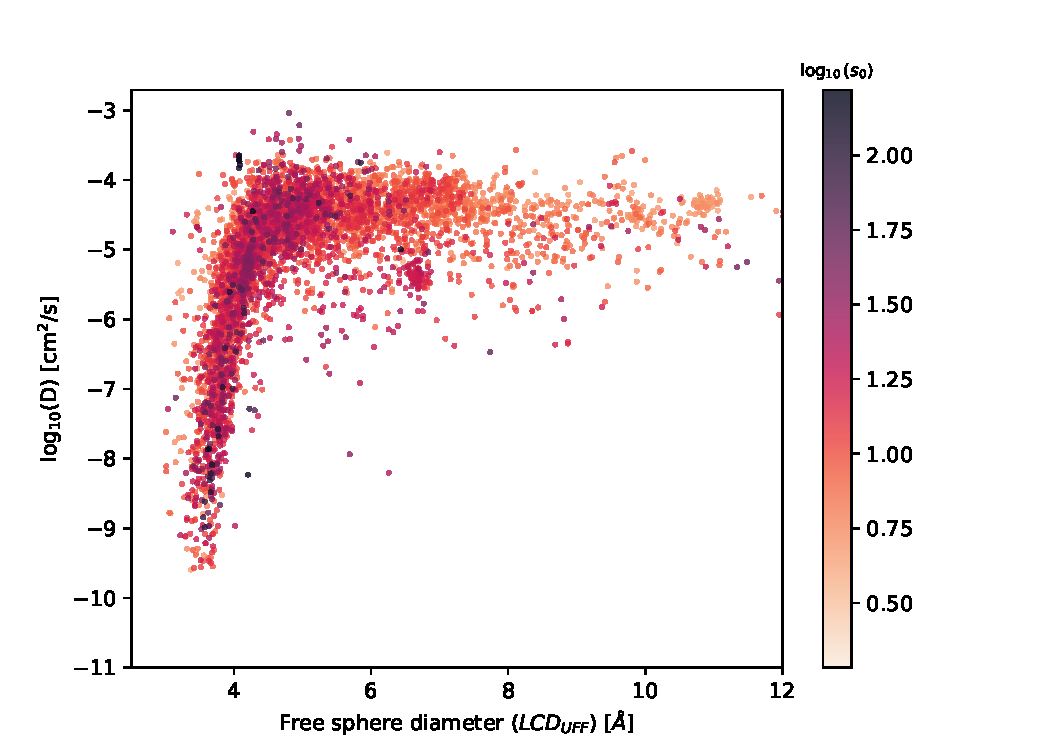
\includegraphics[width=0.48\textwidth]{figures/5-diffusion/D_log-diameter_ccdc_colored_s_+.pdf}
    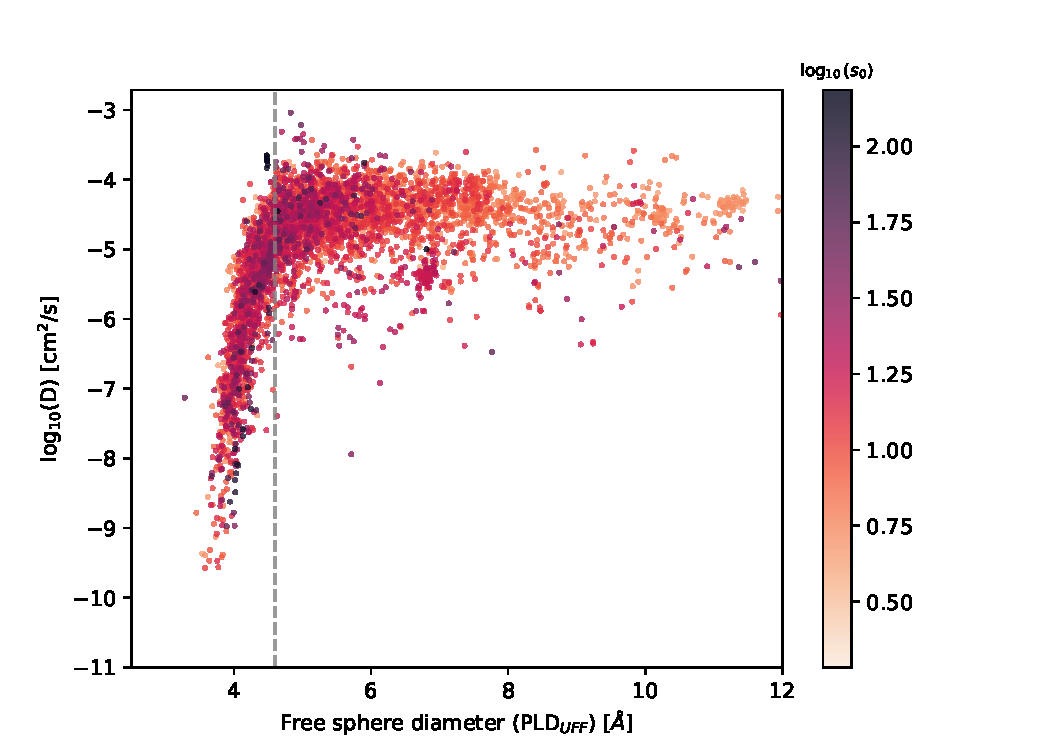
\includegraphics[width=0.48\textwidth]{figures/5-diffusion/D_log-diameter_colored_s_+.pdf}
    \caption{Xenon diffusion coefficient at infinite dilution as a function of the pore limiting diameter (PLD). The diameter of the largest free sphere is defined using two different radius systems: the standard CCDC-based PLD (on the left), and the one defined using the UFF forcefield (on the right)\autocite{Hung_2021} --- as defined in Chapter 2. }\label{fgr:diff_pld}
\end{figure}

If the channel dimensions (determined using Zeo++) are analyzed, partial information regarding the channel shape can be obtained. The dispersion of diffusion coefficients at the plateau depicted in Figure~\ref{fgr:scatter_diffusion_chandim} is challenging to characterize visually based on the channel dimension alone. 

\begin{figure}[ht]
  \centering
    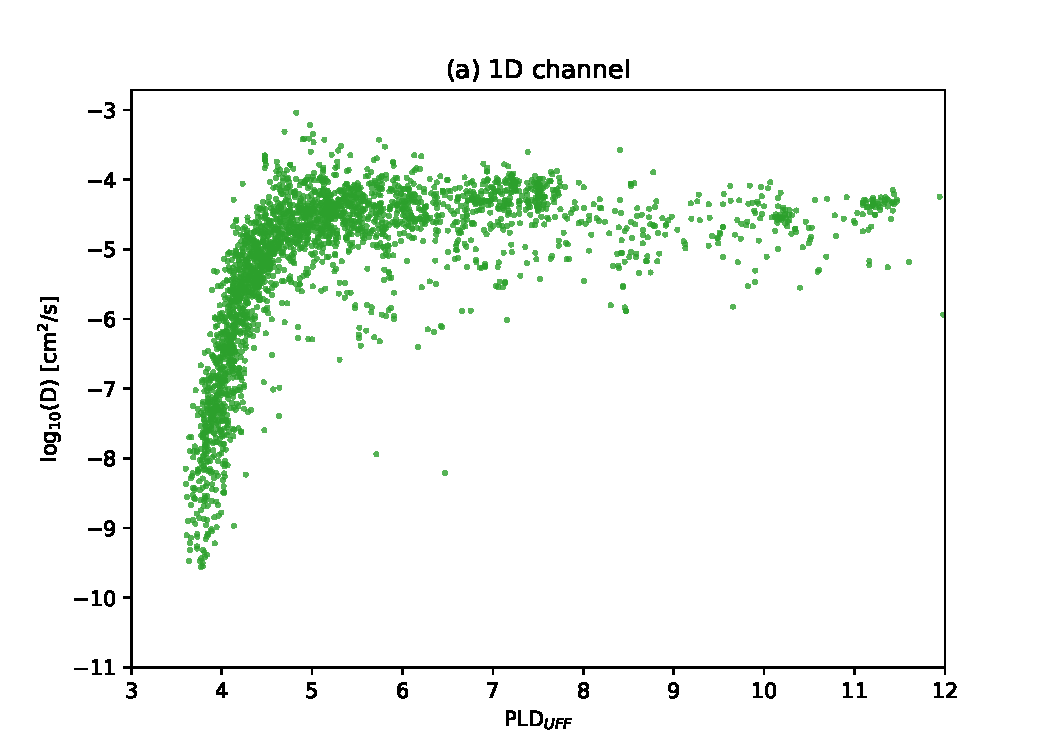
\includegraphics[width=0.32\textwidth]{figures/5-diffusion/D_log-PLD_1D_chan.pdf}
    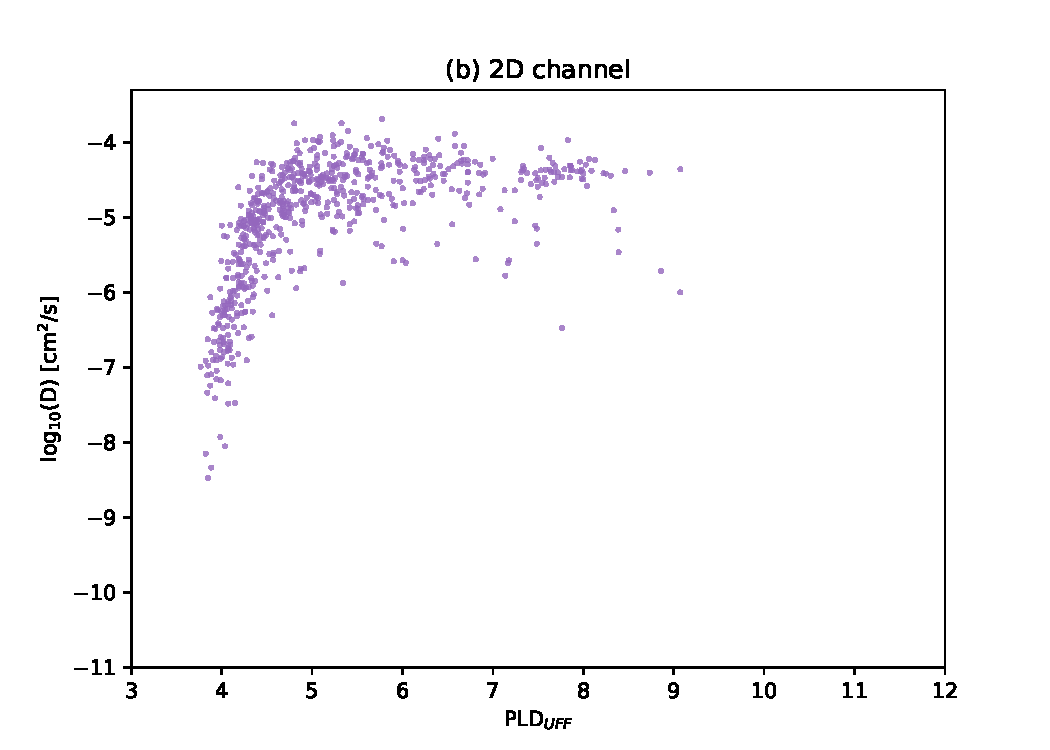
\includegraphics[width=0.32\textwidth]{figures/5-diffusion/D_log-PLD_2D_chan.pdf}
    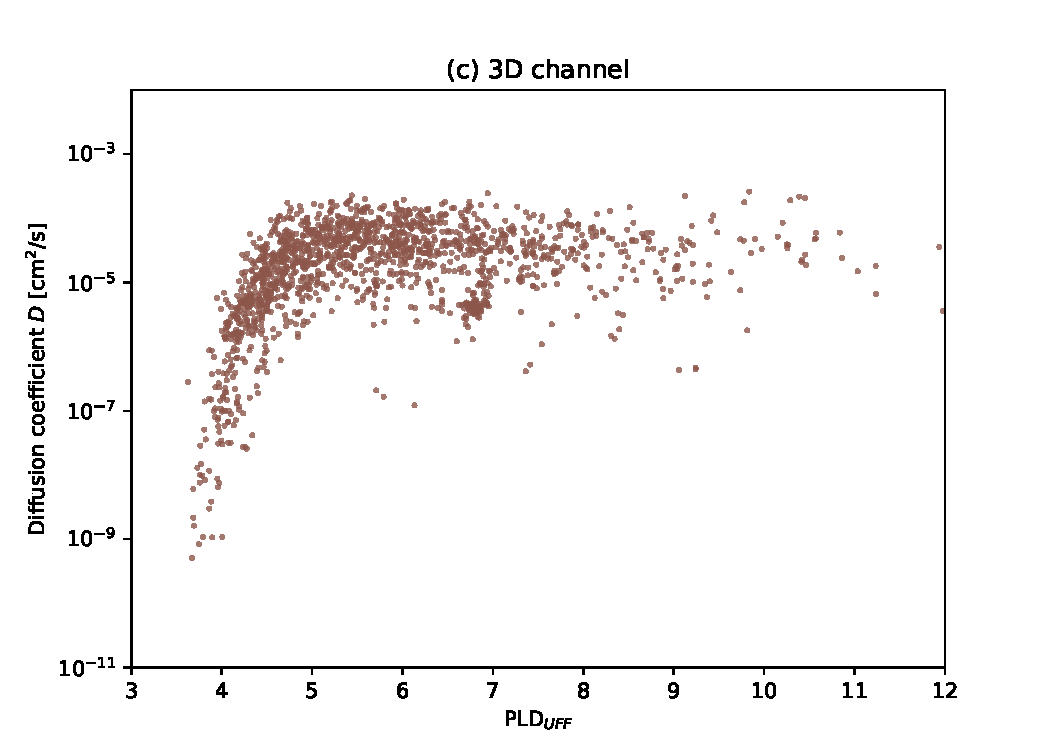
\includegraphics[width=0.32\textwidth]{figures/5-diffusion/D_log-PLD_3D_chan.pdf}
    \caption{ Distributions of the base-10 logarithm of the diffusion coefficients of three different subsets of the screened structures. The first one (a) is composed of structures with a unidimensional channel, the second (b) bidimensional channels and the third one (c) tridimensional channels. }\label{fgr:scatter_diffusion_chandim}
\end{figure}

For this reason, the distribution of diffusion coefficients that depend on the dimensionality of the channels within the framework was plotted in Figure~\ref{fgr:hist_diffusion_chandim}. The distribution for structures containing 1D structures is characterized by a much heavier tail in terms of low diffusion coefficients. Structures with 1D channels are more likely to have very low diffusion coefficients below $3\times 10^{-8}$~\si{\square\cm\per\s}. The vast majority of structures with tridimensional channels tend to have higher diffusion coefficients between $3\times 10^{-6}$~\si{\square\cm\per\s} and $10^{-4}$~\si{\square\cm\per\s}, with almost very few structures having lower diffusion coefficients. The influence of channel dimensionality on diffusion coefficients is not as pronounced for bi- and unidimensional channels. In the case of bi- and unidimensional channels, structures with diffusion coefficients between $3\times 10^{-8}$~\si{\square\cm\per\s} and $3\times 10^{-6}$~\si{\square\cm\per\s} are more common, although less frequent in theory. Therefore, the dimensionality of the channels can influence the values of diffusion coefficients, although the relationship is not as clear as for PLD.

\begin{figure}[ht]
  \centering
    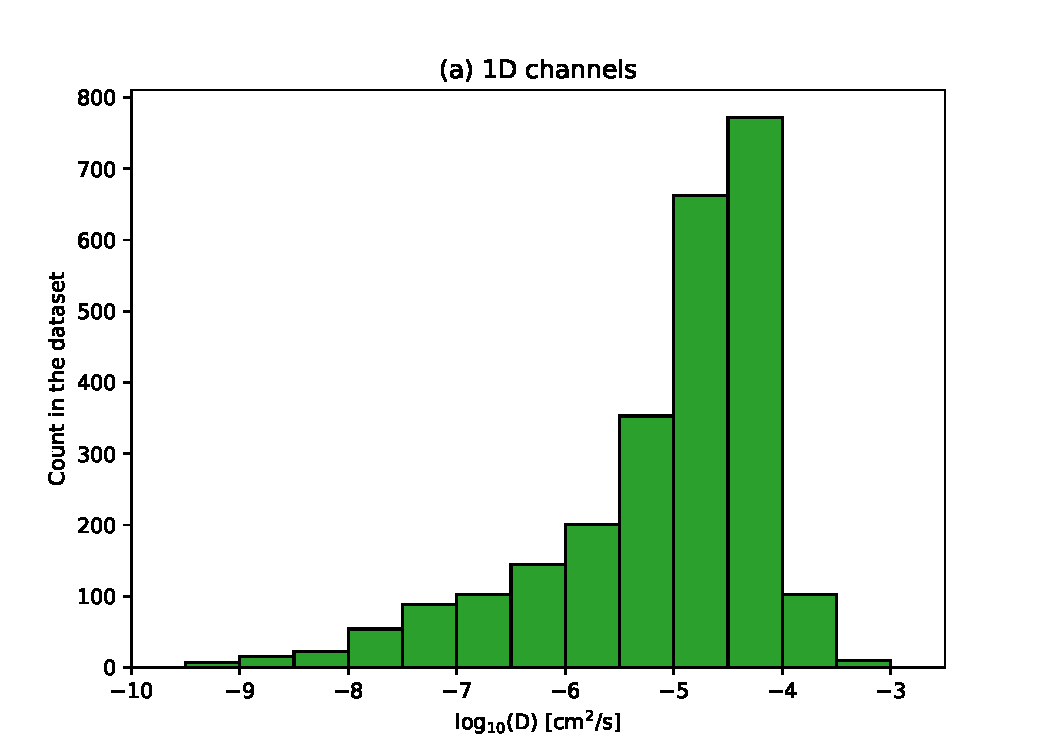
\includegraphics[width=0.32\textwidth]{figures/5-diffusion/histogram_chan1D.pdf}
    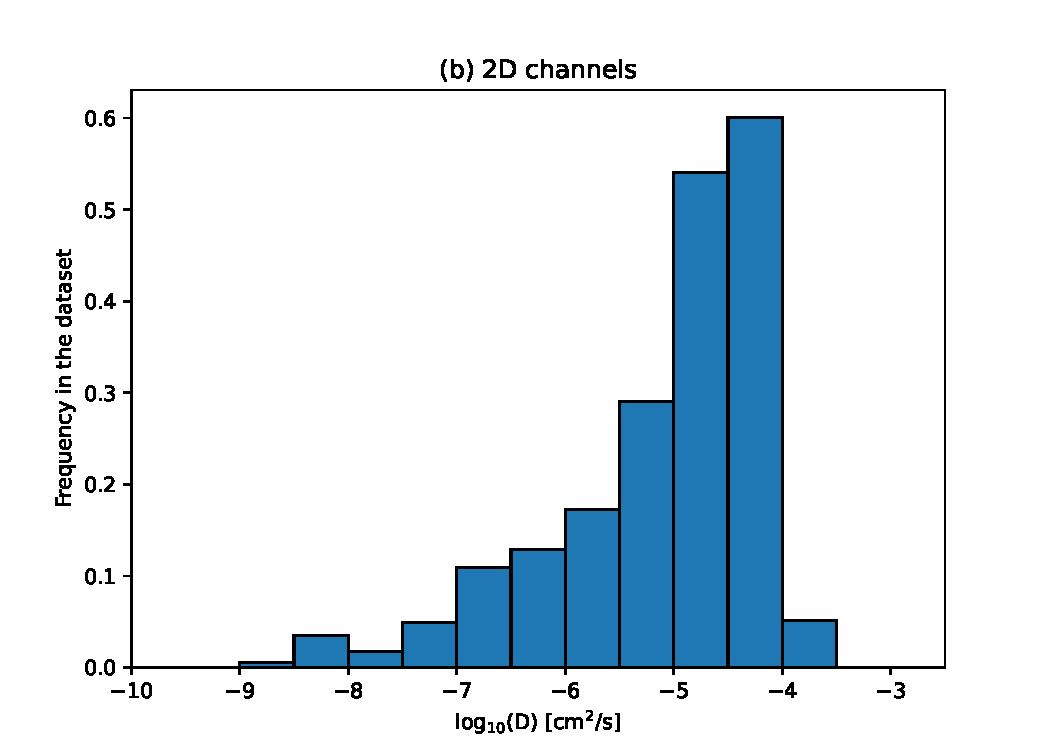
\includegraphics[width=0.32\textwidth]{figures/5-diffusion/histogram_chan2D.pdf}
    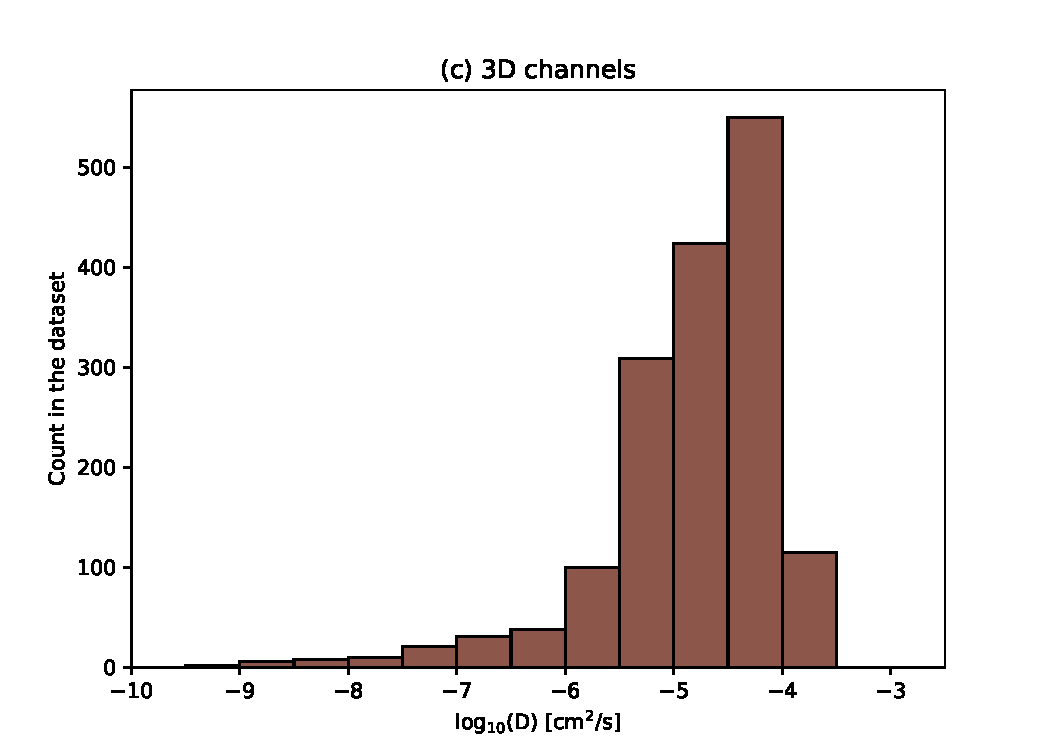
\includegraphics[width=0.32\textwidth]{figures/5-diffusion/histogram_chan3D.pdf}
    \caption{ Distributions of diffusion coefficient of three different subsets of the screened structures. The first one (a) is composed of structures with a unidimensional channel, the second (b) bidimensional channels and the third one (c) tridimensional channels. }\label{fgr:hist_diffusion_chandim}
\end{figure}

Other geometric properties of the material, such as void fraction and surface area, can also influence diffusion. Low diffusion coefficients are typically observed in materials with small pore volumes below $0.6$, as shown in Figure~\ref{fgr:diff_sa_vf}. However, establishing a direct relationship between void fraction and diffusion coefficient is challenging. The only discernible relationship is that materials with void fractions higher than $0.6$ have diffusion coefficients exceeding $3\times 10^{-6}$\si{\square\cm\per\s}. This phenomenon is certainly due to the correlation between PLD and void fraction, as larger PLD values are usually associated with higher void fractions. On the other hand, the accessible surface area for a probe of size $1.2$\si{\angstrom} does not appear to significantly influence the diffusion coefficient.

\begin{figure}[ht]
  \centering
    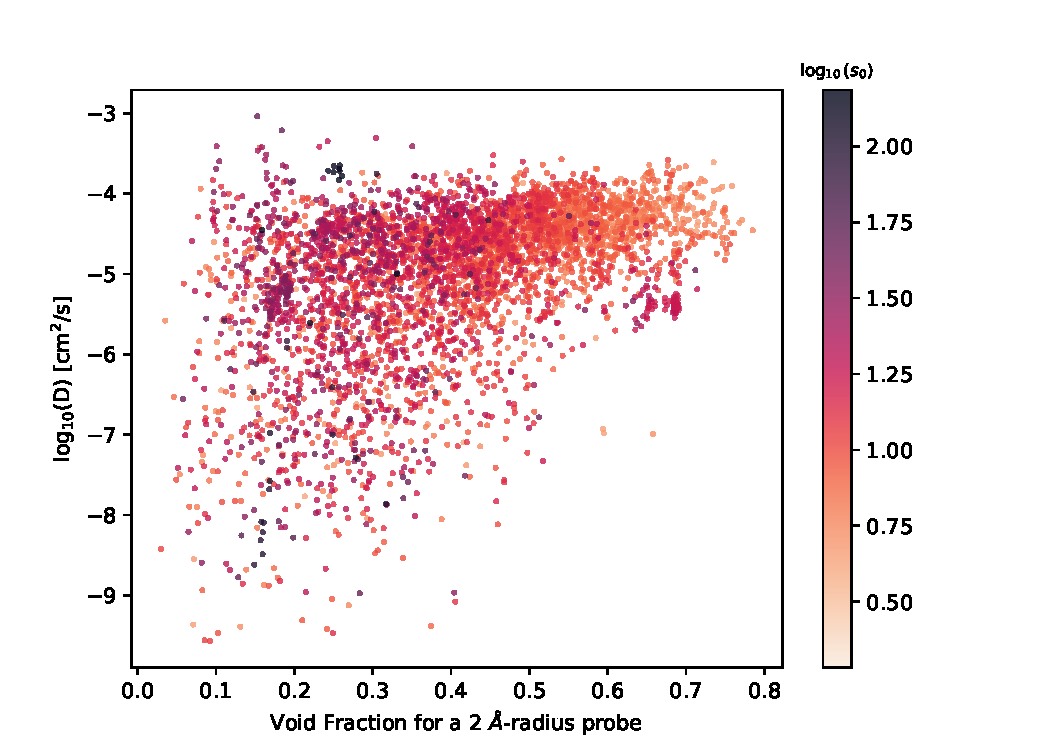
\includegraphics[width=0.48\textwidth]{figures/5-diffusion/D_log-vf_2_s_+.pdf}
    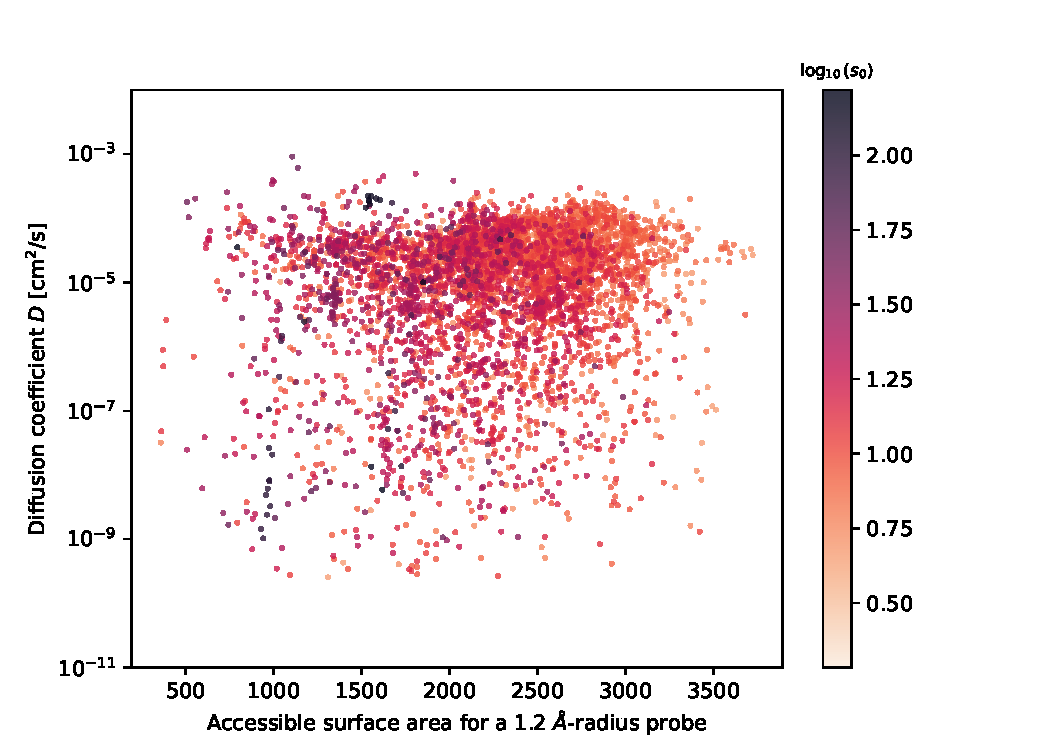
\includegraphics[width=0.48\textwidth]{figures/5-diffusion/D_log-sa_12_s_+.pdf}
    \caption{Xenon diffusion coefficient at infinite dilution as a function of the accessible surface area (left) and the void fraction (right). }\label{fgr:diff_sa_vf}
\end{figure}

Framework density and molar mass are immediate characteristics of the structure that do not require complicated simulations to obtain. However, their relation to the diffusion coefficient is not as straightforward, as shown in Figure~\ref{fgr:diff_density_mass}. It can be inferred that low-density values favor high diffusion coefficients, which can be explained by the logical relation between low density and high porosity. On the other hand, there does not seem to be any clear relationships between the molar mass of the framework and the diffusion coefficients, and no simple geometric or physical reasoning would justify any.

\begin{figure}[ht]
  \centering
    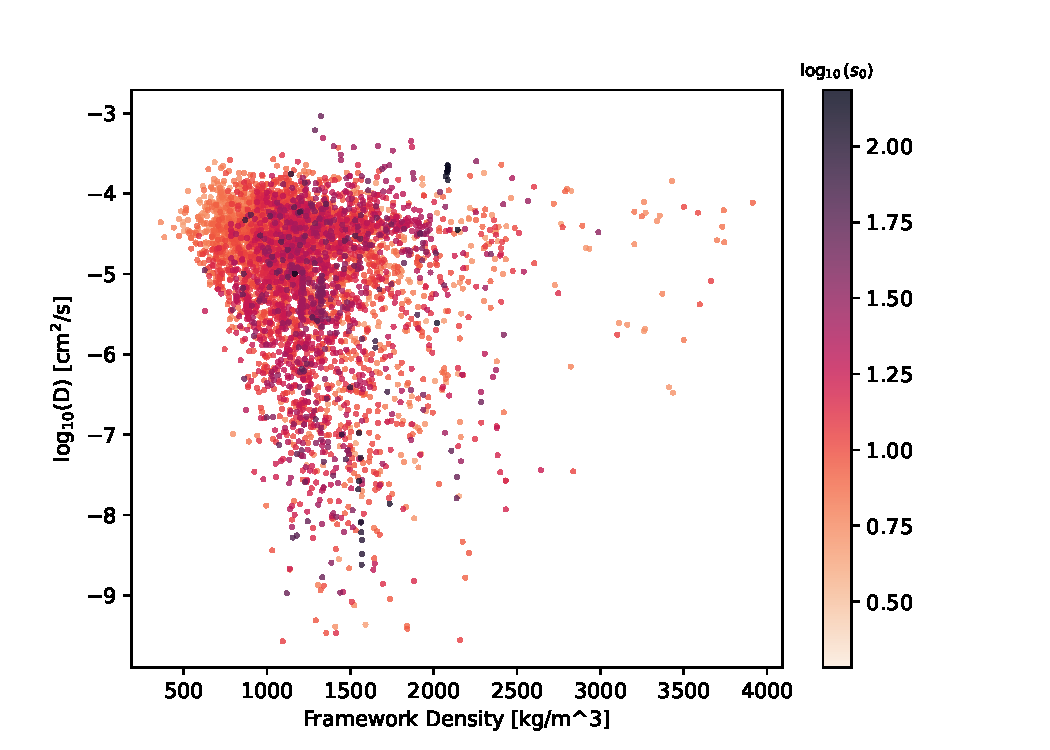
\includegraphics[width=0.48\textwidth]{figures/5-diffusion/D_log-density_s_+.pdf}
    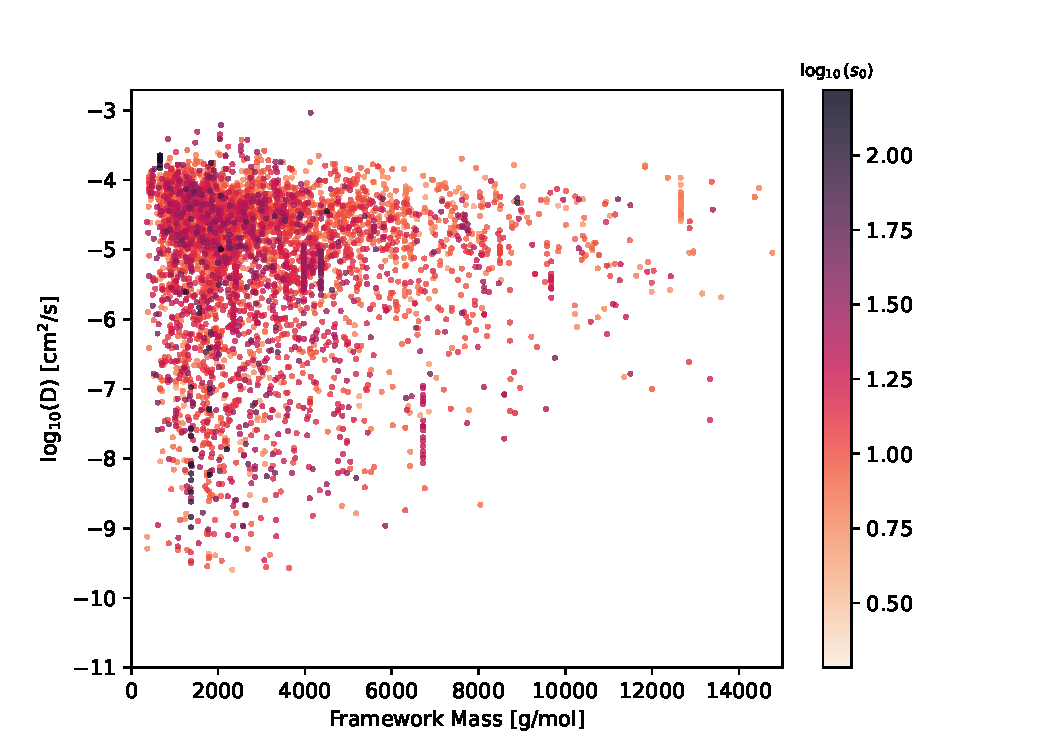
\includegraphics[width=0.48\textwidth]{figures/5-diffusion/D_log-mass_s_+.pdf}
    \caption{Xenon diffusion coefficient at infinite dilution as a function of the density (left) and the mass (right) of the frameworks. }\label{fgr:diff_density_mass}
\end{figure}

The largest sphere diameter D$_{if}$ along a free diffusion path exhibits a similar relationship to the diffusion coefficient, although the correlations are noisier, as depicted in the left plot of Figure~\ref{fgr:diff_H_lcd}. This can be explained by the fact that D$_{if}$ is always equal to or greater than the pore limiting diameter D$_{f}$ by definition. When both diameters are equal, the relationship resembles that shown in Figure~\ref{fgr:diff_pld}, with a linear correlation and a plateau. However, when it is higher, it creates the observed noise pattern in the left plot of the Figure~\ref{fgr:diff_H_lcd}. 

\begin{figure}[ht]
  \centering
    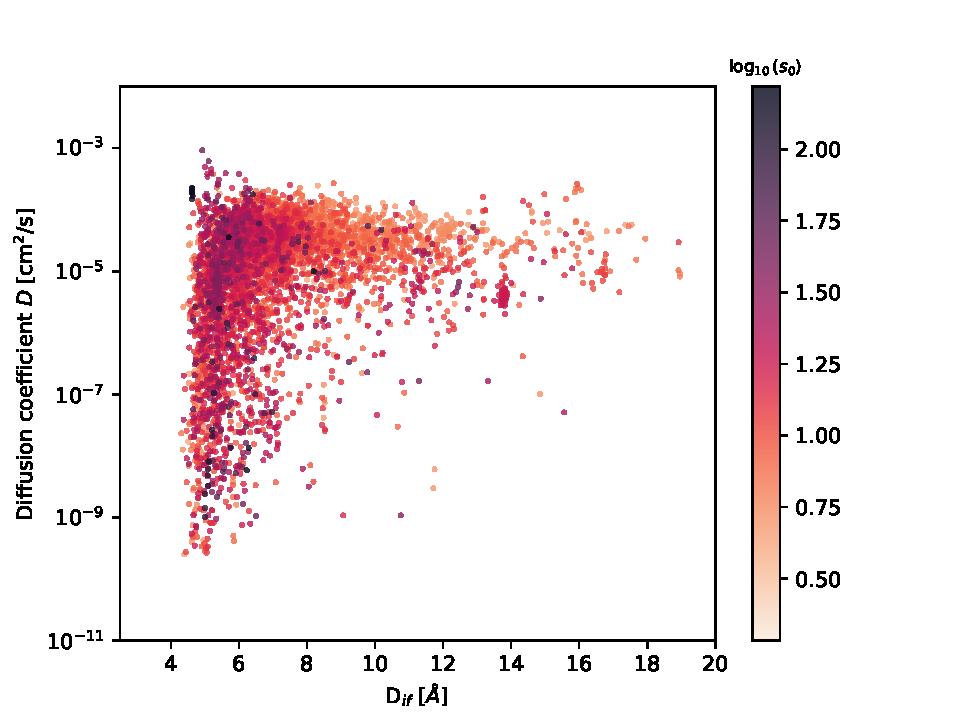
\includegraphics[width=0.48\textwidth]{figures/5-diffusion/D_log-lcd_s_+.pdf}
    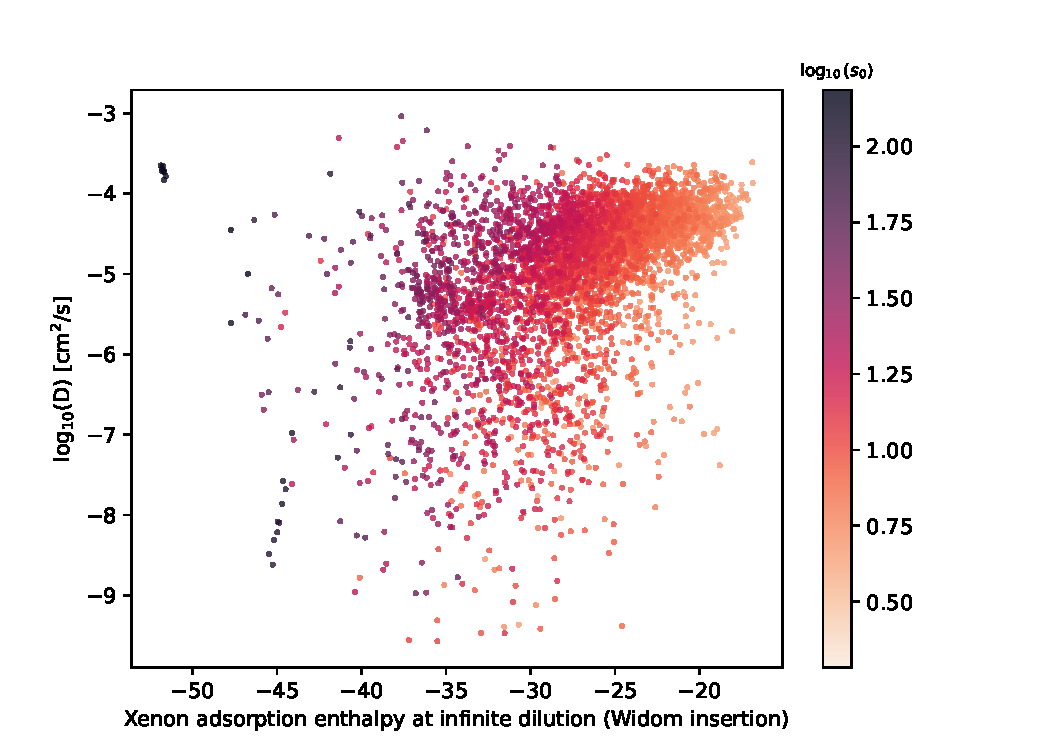
\includegraphics[width=0.48\textwidth]{figures/5-diffusion/D_log-H_Xe_s_+.pdf}
    \caption{Xenon diffusion coefficient at infinite dilution as a function of the largest sphere diameter D$_{if}$ along a free diffusion path (left) and the xenon adsorption enthalpy (right). }\label{fgr:diff_H_lcd}
\end{figure}

A final comparison involves a thermodynamic quantity, namely the xenon adsorption enthalpy $\Delta\e{ads}\ex{Xe}H$. There is no relation between diffusion coefficient and the xenon adsorption enthalpy, which is advantageous for screening because it implies the possibility of various configurations. A high diffusion coefficient and a high xenon adsorption affinity (with very negative enthalpy values) can coexist in a material, which represents the ideal configuration for adsorption at infinite dilution. However, it necessitates testing the diffusivity when the material exhibits good affinity to optimize both properties. This approach will constitute the core discussion regarding the optimization of Xe/Kr selectivity and the diffusion coefficients of Xe and Kr.  

\subsection{A trade-off between the selectivity and the diffusion}

This section analyzes the screening of diffusion and selectivity properties calculated for xenon and krypton to identify relevant materials that demonstrate both a good Xe/Kr selectivity and a good Xe/Kr diffusion coefficient ratio. To achieve this, a diffusion coefficient screening for krypton was performed, resulting in 4,816 structures with a good determination coefficient R$^2$ for both linear fits of xenon and krypton MSD. These structures are subsequently tested to find materials that exhibit a balanced combination of thermodynamic and kinetic properties for xenon/krypton separation.

\subsubsection{Screening of diffusion selectivity values: a trade-off between adsorption and diffusion}\label{sct:diff_screen}

The comparison between xenon/krypton selectivity at infinite dilution and xenon/krypton diffusion coefficients is initiated. Highly selective material can possess a decent diffusion coefficient, indicating that the diffusion limitation observed in the \texttt{KAXQIL} structure is not inevitable, which is encouraging. The left plot of Figure~\ref{fgr:diff_s0_lcd} clearly demonstrates the possibility of all configurations: high selectivity (above $40$) with high diffusion coefficient (over $10^{-6}$~\si{\square\cm\per\s}) and high selectivity with low diffusivity. The krypton coefficients exhibit relative stability between $10^{-6}$~\si{\square\cm\per\s} and $10^{-3}$~\si{\square\cm\per\s}. Consequently, increasing the diffusion selectivity is not the primary leverage for enhancing the diffusion selectivity, as highly selective materials do not display very low krypton diffusion coefficients. To surpass thermodynamic selectivity, a transport-related selectivity metric is examined to identify highly selective materials without significant transport limitations.

\begin{figure}[ht]
  \centering
    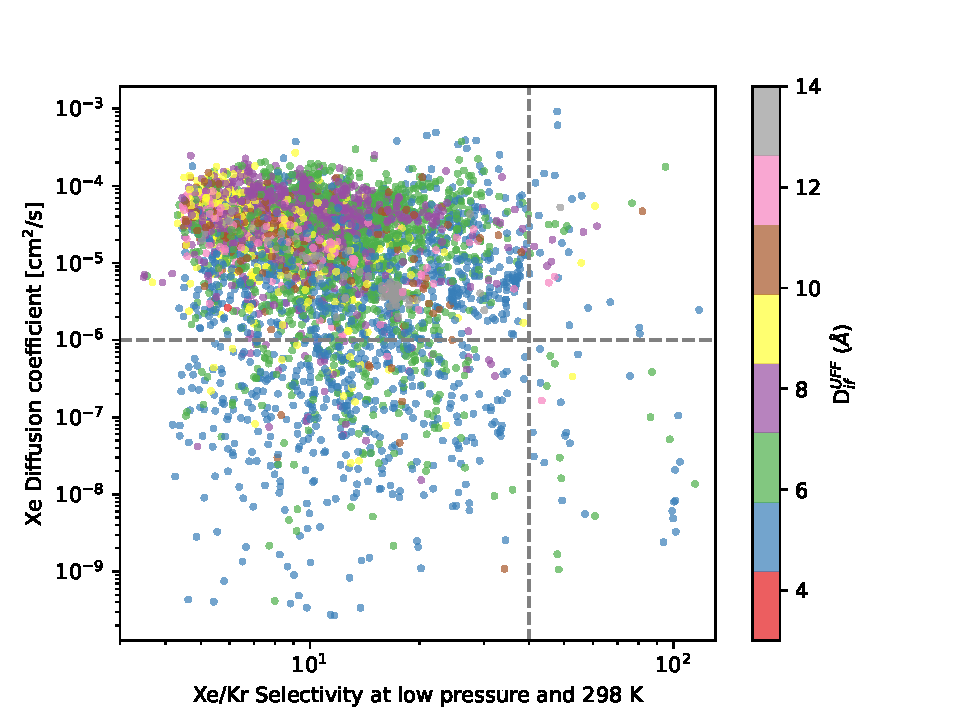
\includegraphics[width=0.48\textwidth]{figures/5-diffusion/D_xe-s0-lcd.pdf}
    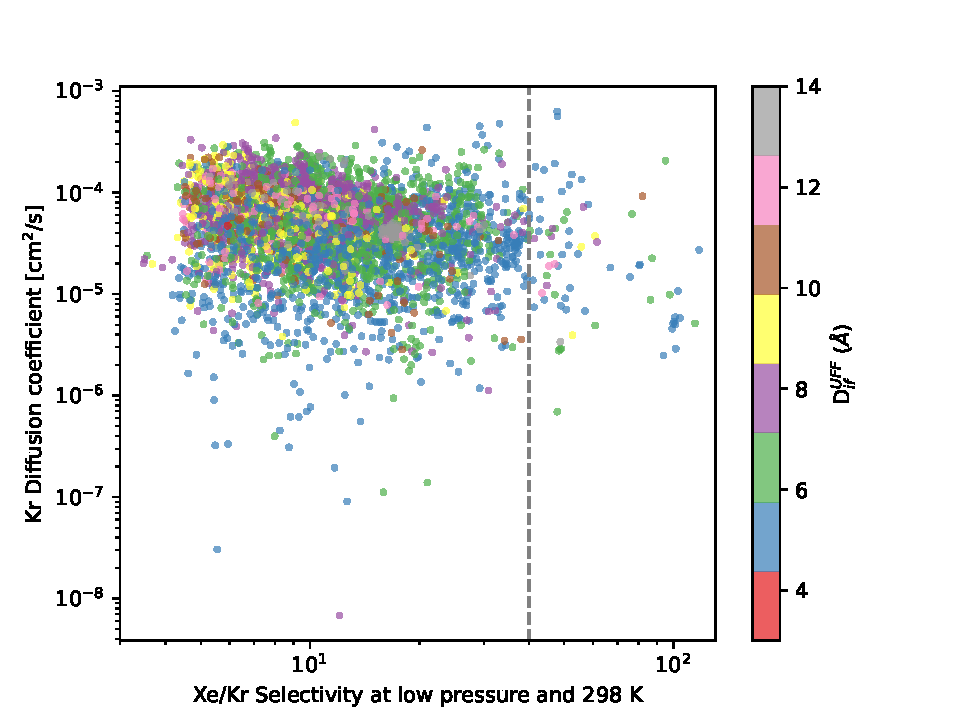
\includegraphics[width=0.48\textwidth]{figures/5-diffusion/D_kr-s0-lcd.pdf}
    \caption{On the left panel, the Xe/Kr diffusion selectivity (ratio of the diffusion coefficients) is plotted against the Xe/Kr selectivity values at infinite diluation (calculated by Widom insertion), and the points are color-coded by the largest cavity diameter within a diffusion path D$_{if}$. On the right panel, the same plot is now color-coded with the average dimension of the channels of the nanoporous structures associated. }\label{fgr:diff_s0_lcd}
\end{figure}

The transport properties in a separation process are generally evaluated using the ratio of diffusion coefficients or the diffusion selectivity as performance metrics. For xenon and krypton, the diffusion selectivity can be defined as follows:\autocite{Krishna_2010}
\begin{equation}
  s\ex{Xe/Kr}\e{diff} = \frac{D\ex{Xe}}{D\ex{Kr}}
\end{equation}
To consider both transport and thermodynamic effects, the thermodynamic adsorption selectivity defined in Chapter 2 (equations~\ref{eq:selec_0} and~\ref{eq:selec_0}) is combined with the diffusion selectivity to define the membrane selectivity (used to characterize membranes). This membrane selectivity can also be referred to as permselectivity, as it corresponds to the ratio of permeabilities of the components in the binary mixture targeted for separation. The xenon/krypton permselectivity ($s\ex{Xe/Kr}\e{perm}$) can thus be defined as follows:
\begin{equation}\label{eq:membrane_selec}
  s\ex{Xe/Kr}\e{perm} = s\ex{Xe/Kr}\e{diff} \times s\ex{Xe/Kr}\e{ads}
\end{equation}
where $s\ex{Xe/Kr}\e{ads}$ corresponds to the adsorption selectivity used throughout the previous chapters (at infinite dilution or higher pressure). 

\begin{figure}[ht]
  \centering
    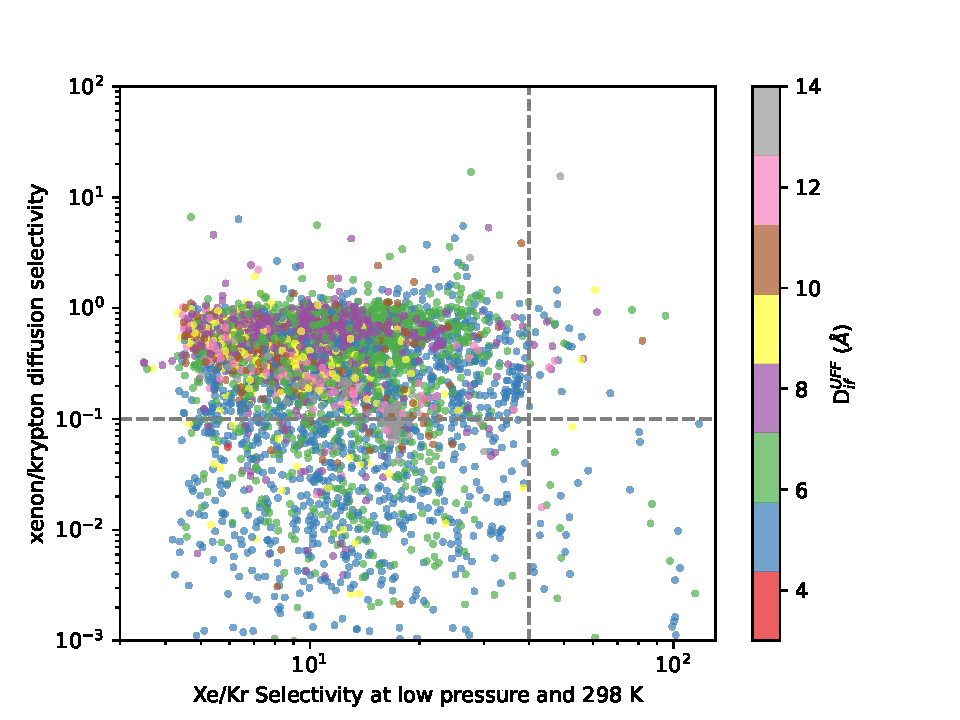
\includegraphics[width=0.48\textwidth]{figures/5-diffusion/diff_D_xekr-s0-lcd.pdf}
    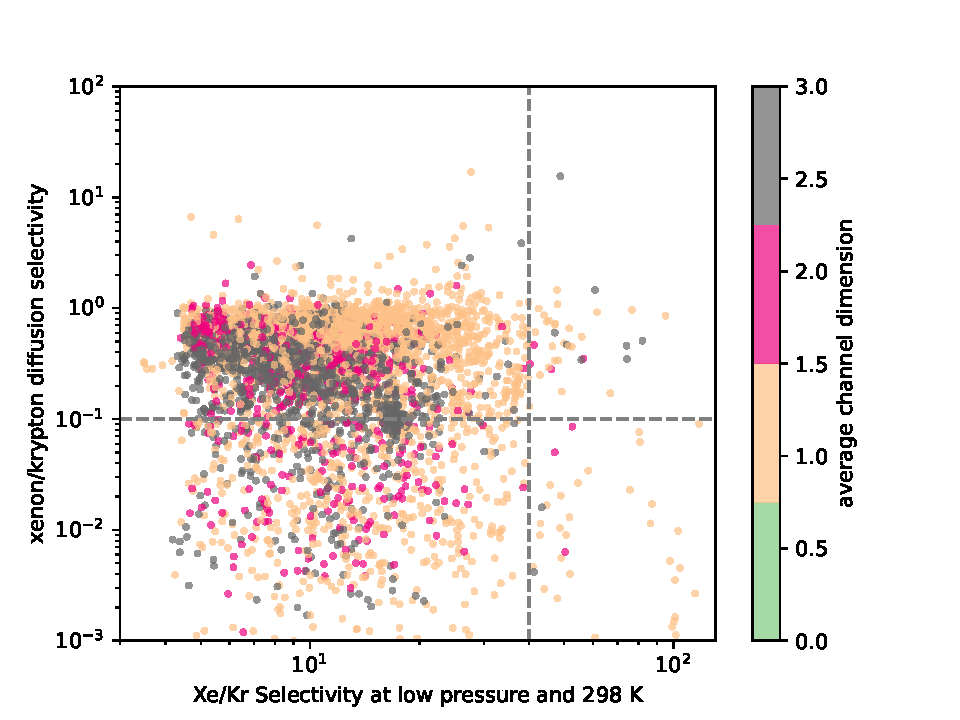
\includegraphics[width=0.48\textwidth]{figures/5-diffusion/diff_D_xekr-s0-chandim.pdf}
    \caption{}\label{fgr:perm_selec0}
\end{figure}

Using both $s\ex{Xe/Kr}\e{diff}$ and $s\ex{Xe/Kr}\e{ads}$ at different pressure conditions, this study will try to find materials that exhibit a relatively high selectivity with high diffusion selectivity. The plots presented in Figure~\ref{fgr:perm_selec0} demonstrate that a total of 48 structures display a selectivity above $40$, along with a good diffusion selectivity over $0.1$. Notably, these structures possess rather large pore sizes, represented by the largest included sphere along a free diffusion path $D_{if}$ as depicted in the left plot of Figure~\ref{fgr:perm_selec0}. Additionally, these large pores are associated with structures that exhibit various dimensionalities. Among these structures, one particular standout is characterized by exceptionally high diffusion selectivity (over $15$, as indicated by the gray point on the upper right side of the left plot of Figure~\ref{fgr:perm_selec0}) coupled with a high adsorption selectivity at infinite dilution. It is worth mentioning that this structure, with a CSD code \texttt{ADOGEH}\cite{Peikert_2012}, features a three-dimensional channel framework with large pores and relatively narrow connecting channels. However, the high adsorption selectivity observed at infinite dilution is not maintained under ambient pressure conditions, as illustrated in Figure~\ref{fgr:perm_selec2080} (refer to Table~\ref{table:diff} for further details).

Upon closer examination of these 48 structures, it becomes evident that they incorporate a combination of large and small pores, such that the diffusion is not obstructed, while achieving high selectivity within more confined spaces. Materials with varying pore sizes of this nature may experience a decrease in selectivity at higher pressures, as larger pores are less selective and become accessible as the gas pressure increases. This phenomenon is apparent when comparing the plots with those presented in Figure~\ref{fgr:perm_selec2080}.

\begin{figure}[ht]
  \centering
    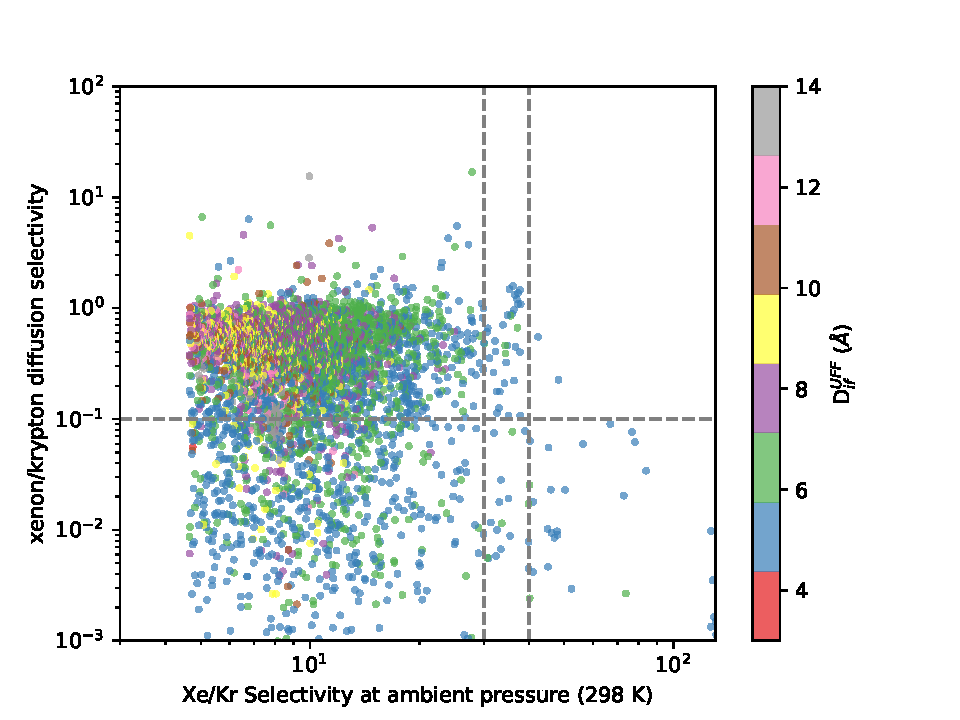
\includegraphics[width=0.48\textwidth]{figures/5-diffusion/diff_D_xekr-s2080-lcd.pdf}
    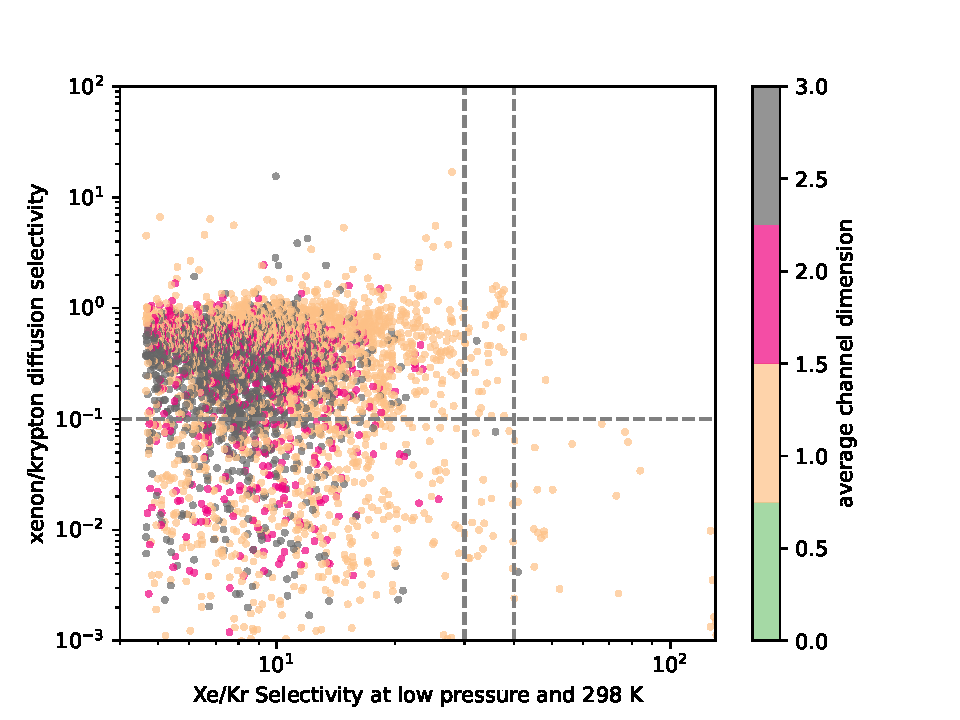
\includegraphics[width=0.48\textwidth]{figures/5-diffusion/diff_D_xekr-s2080-chandim.pdf}
    \caption{The xenon/krypton diffusion selectivity plotted against the ambient-pressure selectivity for a 20:80 Xe/Kr composition and color-coded by the LCD within a diffusion path D$_{if}$ (left panel) and by the average dimension of channels (right panel). }\label{fgr:perm_selec2080}
\end{figure}


At higher pressure, a shift towards lower selectivity values is observed in some materials. It is noteworthy that only 2 structures exhibit an ambient-pressure selectivity exceeding $40$: the MOFs with the CSD codes \texttt{XUNSOQ}\autocite{Abrahams_2014} and \texttt{GUMDEZ}\autocite{Yin_2014} (Table~\ref{table:diff}). Most of these materials demonstrate a high cavity size, with only structures having an LCD near \SI{6}{\angstrom} remaining in this area of the plot. Furthermore, the channel dimension is also equal to one, providing a glimpse into the characteristics of these intriguing materials. They are made of unidimensional channels with small pore sizes, enabling the preservation of selectivity even under higher pressure conditions. Expanding the scope to structures with a selectivity higher than $30$ (instead of $40$), a total of 38 structures share similar features, including relatively low pore sizes and low channel dimensionality. Some of these structures, like \texttt{QOZDOY}\autocite{Zhang_2001}, have managed to maintain their selectivity to a certain extent, despite not being detected during the pre-screening based on low-pressure selectivity (Figure~\ref{fgr:perm_selec0}). However, other structures, such as the MOF \texttt{MISQIQ}\autocite{Tong_2013}, have experienced a significant drop in selectivity values from infinite dilution to ambient pressure (see Table~\ref{table:diff}).

When considering ambient-pressure selectivity, the large majority of highly selective materials actually have relatively low diffusion selectivity values (lower than $0.1$), as shown in Figure~\ref{fgr:perm_selec2080} (this was not the case for low-pressure selectivity). This result suggests the necessity of a trade-off between adsorption selectivity and diffusion selectivity. In the screening approach undertaken in this thesis, the decision was made to lower the adsorption diffusivity to approximately $40$ to attain higher diffusion selectivity values. This choice was motivated by the fact that previous literature screenings \autocite{Simon_2015,Chung_2019} and the author's own published work~\cite{Ren_2021} solely focused on maximizing adsorption selectivity --- this corresponds to working on the lower right side of the plots in Figure~\ref{fgr:perm_selec2080}. To improve upon the previous approach, a kinetic constraint was included in the screening process. An alternative approach consists in optimizing the permselectivity, also known as membrane selectivity (equation~\ref{eq:membrane_selec}). However, this would address a different application, namely membrane separation, which is extensively studied in the literature\autocite{Anderson_2017,Wang_2022}. In the presented screening, the objective was to identify thermodynamically selective materials that are not limited by diffusion. Several interesting materials were identified and will be further examined in the following subsection.


\subsubsection{Identification of interesting materials}

By cross-referencing the transport data with the thermodynamic data, it is possible to optimize the Xe/Kr adsorption selectivity while imposing a constraint on the diffusion selectivity to ensure it falls within an acceptable range (above $0.1$). The structures of the 65 materials exhibiting a low-pressure Xe/Kr selectivity higher than $40$ or an ambient-pressure Xe/Kr selectivity higher than $30$ were manually visualized and briefly analyzed. Different materials were hand-picked for further analysis based on their unique characteristics. Materials with dissimilar types of channels that can artificially yield high diffusion coefficients were discarded. This phenomenon arises due to the randomness of the initial conditions. For instance, when xenon diffuses in a wider channel while krypton diffuses in a narrower channel, the diffusion selectivity will inevitably be artificially higher. One example is the MOF with a CSD code \texttt{OQESAF}\autocite{Xie_2011}, which was affected by this phenomenon, as shown in Figure~\ref{fgr:OQESAF}, where different diffusion coefficient values are observed depending on the channel considered (in this case, a Henry coefficient weighted average needs to be performed). Other materials exhibit moderately high diffusion selectivity values ($\lesssim 1$) and typically consist of unidimensional channels that allow relatively free diffusion of xenon (higher than \SI{4.6}{\angstrom}) with varying cavity sizes. Multiple factors appear to influence the diffusion coefficients, including the values of channel size and pore size, but notably, the shape of the channel composed of cavities connected by narrower walls also plays a crucial role. The tortuosity of the layout and the relative difference between the cavities and the connecting channels can lead to significant variations in diffusion properties.

\begin{figure}[ht]
  \centering
    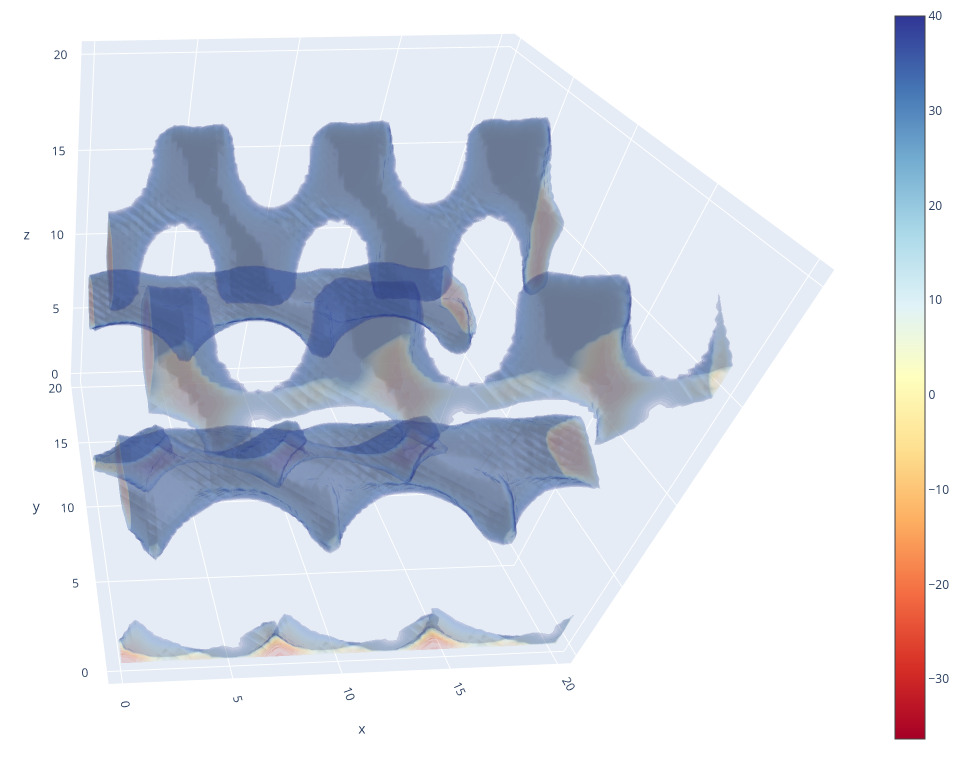
\includegraphics[height=0.4\textwidth]{figures/5-diffusion/viz/OQESAF.jpg}
    \caption{Snapshot of a 3D visualization of the xenon interaction energy inside the channels of the \texttt{OQESAF}\autocite{Xie_2011} material. Two distinct unidimensional channels can be observed in the visualization. In an MD simulation of a single xenon per box, in this study, all possible initial positions were not tested out. }\label{fgr:OQESAF}
\end{figure}

In this section, a detailed analysis of the comparative transport and adsorption performances of selected representative structures (Table~\ref{table:diff}) will be conducted to gain a better understanding of the key factors contributing to the observed differences in performance. This work can be used to design more quantitative characteristics that explain better transport performance, similar to the approach employed for the thermodynamic screening, which resulted in the identification of essential thermodynamic descriptors used in the design of an ML model for adsorption selectivity prediction (chapters 3--4). To achieve this, a visualization tool based on the grid calculation principle discussed in the dedicated section~\ref{sct:grid} will be employed, and the corresponding code is available in the same Github repository: \url{github.com/coudertlab/GrAED}.

\begin{table}[ht]
\small
\setlength\extrarowheight{2pt}
\centering
\begin{tabular}{|l|c|c|c|c|c|c|c|}
\hline
  Structure &       &    &  Pore size &  Channel size   &     & Diffusion Coeff. & Xe uptake \\
  CSD ref.\ code &  $s_0\ex{Xe/Kr}$  &  $s_1\ex{Xe/Kr}$   &    D$_{if}\ex{UFF}$ (\si{\angstrom})   &   PLD\ex{UFF} (\si{\angstrom})  &  $s\e{diff}\ex{Xe/Kr}$ &  $D\e{diff}\ex{Xe}$ (\si{\square\centi\meter\per\second}) & (\si{\milli\mole\per\gram}) \\
\hline
\texttt{OQESAF}~\cite{Xie_2011} & 28 & 28 &  5.8 & 5.0 &  17 &  4$\times$10\ex{-5} & 3.2 \\
\hline
\texttt{ADOGEH}~\cite{Peikert_2012} & 49  &  10 & 12.9 & 5.3 & 15.5 &  5$\times$10\ex{-5} & 1.7 \\
\hline
\texttt{KAXQIL}~\cite{Banerjee2012} & 104  & 133 &  5.2 & 4.1 &  0.005 &  3$\times$10\ex{-8}  & 1.4 \\
\texttt{XUNSOQ}~\cite{Abrahams_2014} & 38  & 48 &  5.6 & 4.8 &  0.23 &  7$\times$10\ex{-6} & 3.5 \\
\texttt{BAEDTA01}~\cite{Chen_2010} & 152 & 38 &  5.7 & 4.6 &  0.4 &  4$\times$10\ex{-5} & 1.1 \\
\texttt{TONBII}~\cite{Du_2010} & 44 & 35 &  5.1 & 4.8 &  0.86 &  1$\times$10\ex{-4} & 1.5 \\
\hline
\texttt{VOHQIS}~\cite{Wragg_2001} & 51 & 48 &  5.7 & 3.9 &  0.01 &  6$\times$10\ex{-8} & 2.6\\
\texttt{QOZDOY}~\cite{Zhang_2001} & 52  & 37 &  5.6 & 5.0 &  0.45 &  7$\times$10\ex{-5} & 3.7 \\
\texttt{GUMDEZ}~\cite{Yin_2014} & 56 & 42 &  5.5 & 5.1 &  0.55 &  7$\times$10\ex{-5} & 3.0 \\
\texttt{MISQIQ}~\cite{Tong_2013} & 140 & 37 &  4.6 & 4.5 &  1.4 &  2$\times$10\ex{-4} & 2.3 \\
\hline
\end{tabular}
\caption{Transport and thermodynamic performances of top-performing structures of CoRE MOF 2019 screened out by the approach developed in the section~\ref{sct:diff_screen}. The thermodynamic properties are determined using xenon uptake at \SI{1}{\bar} and \SI{298}{\kelvin}, $s_0\ex{Xe/Kr}$ and $s_1\ex{Xe/Kr}$ that correspond to the xenon/krypton adsorption selectivity values respectively at infinite dilution and ambient pressure condition. The pore size is defined as the largest cavity along a free diffusion path D$_{if}\ex{UFF}$ and the channel size is defined using the pore limiting diameter PLD\ex{UFF} using atom radii defined by the UFF. The transport properties are evaluated using the xenon/krypton diffusion selectivity $s\e{diff}\ex{Xe/Kr}$ and the xenon diffusion coefficient $D\e{diff}\ex{Xe}$ calculated by the MD-based screening presented above. }\label{table:diff}
\end{table}

The structure \texttt{ADOGEH}\autocite{Peikert_2012}, an amino-substituted version of the well-known HKUST-1 or Cu$_3$(btc)$_2$ (btc = 1,3,5-benzenetricarboxylate), was not found when comparing the transport data with the ambient-pressure selectivity values and the infinite dilution selectivity values, which explains that the selectivity $s_1$ for this structure is relatively low ($10$) compared to other materials (over $35$). However, \texttt{ADOGEH} was detected when considering the selectivity $s_0$ at infinite dilution due to its exceptional diffusion selectivity (around $10$). This suggests that as a membrane material, \texttt{ADOGEH} could exhibit a selectivity of approximately $100$, one of the highest values observed. Even as an adsorption-based separation material, it demonstrates an outstanding low-pressure selectivity of $49$ coupled with its high diffusion selectivity, making it suitable for certain applications involving very low partial pressures of xenon and krypton.

\begin{figure}[ht]
  \centering
  \begin{subfigure}[b]{0.45\textwidth}
    \centering
    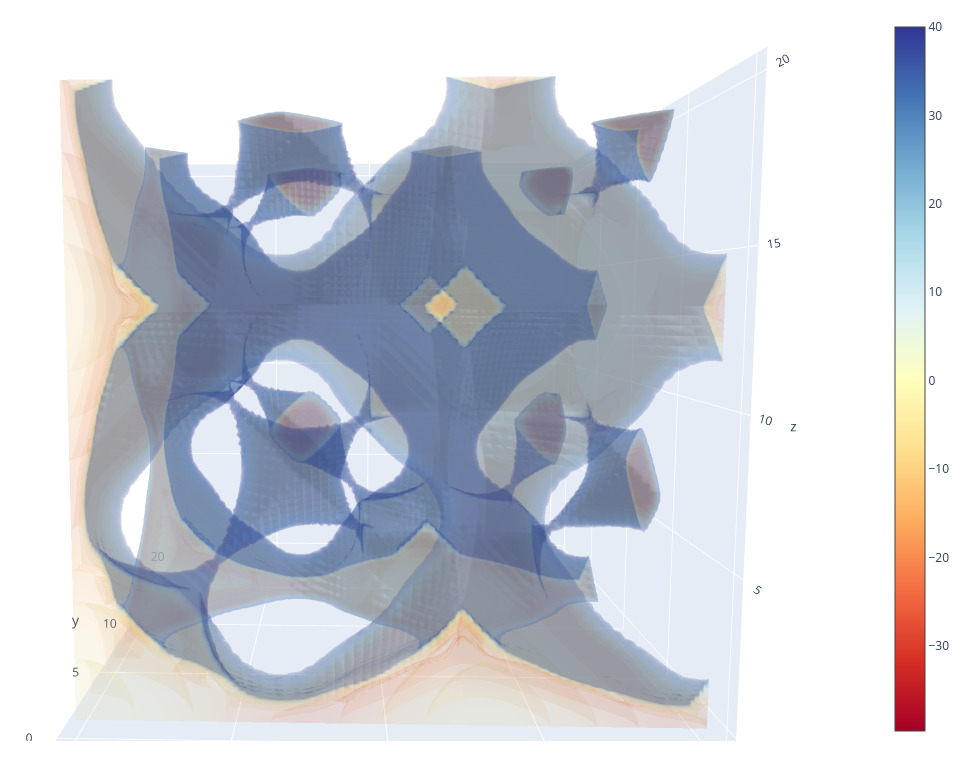
\includegraphics[width=\textwidth]{figures/5-diffusion/viz/ADOGEH_Xe.jpg}
    \caption{Xe energy grid in \texttt{ADOGEH}}\label{fgr:ADOGEH_Xe}
  \end{subfigure}
  \hspace{1cm}
  \begin{subfigure}[b]{0.45\textwidth}
    \centering
    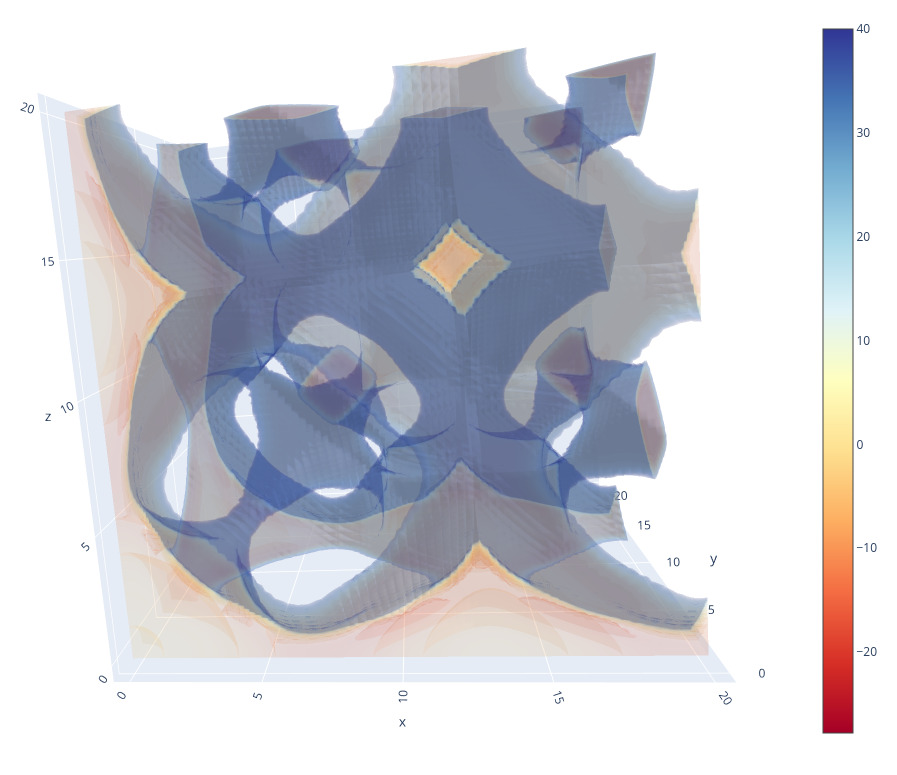
\includegraphics[width=\textwidth]{figures/5-diffusion/viz/ADOGEH_Kr.jpg}
    \caption{Kr energy grid in \texttt{ADOGEH}}\label{fgr:ADOGEH_Kr}
  \end{subfigure}
  \caption{3D volume plot of the xenon (a) and krypton (b) interaction energy values inside the material \texttt{ADOGEH}\autocite{Peikert_2012} calculated using an energy grid as described in the section~\ref{sct:grid}. }\label{fgr:ADOGEH}
\end{figure}

Even when used as an experimental material, the diffusion properties of xenon and krypton in this material are of significant interest in themselves. It was observed that only two materials displayed a diffusion selectivity over $10$ in Figure~\ref{fgr:perm_selec0}. However, the other material has an artificially high diffusion selectivity due to the above-mentioned randomness of the initial position in the MD simulation and the presence of two types of channels (refer to Figure~\ref{fgr:OQESAF}). Among all the screened materials for diffusion performance, \texttt{ADOGEH} stands out as the material with the highest diffusion selectivity. In a unidimensional system, it is more natural to expect a higher or equivalent diffusion coefficient for krypton compared to xenon due to their significant size difference.

This noteworthy behavior of adsorption  \texttt{ADOGEH} can be explained by a special mechanism occurring in its tridimensional channel network. As depicted in Figure~\ref{fgr:ADOGEH}, both xenon and krypton have access to all dimensions for diffusion through the channels in the three directions of space. However, when examining the type of ``pocket'' that connects the channels diagonally, it becomes apparent that the access differs when comparing the two 3D energy grid plots. This pocket can be accessed by a xenon or a krypton atom even if the energy barrier to cross is relatively high. Figure~\ref{fgr:ADOGEH_Xe} shows that the connection is narrower for xenon compared to krypton at the same energy threshold, which implies a higher energy barrier for xenon to access the ``pocket'' compared to krypton. This discrepancy in energy barrier explains the unusual difference in diffusion coefficients between xenon and krypton since krypton has a greater number of diffusion directions of space available than xenon, increasing the probability of turning around, which slows krypton down on the long run. In other words, xenon can diffuse in the 3D space using only three main directions, while krypton deviates from the main channel axes. Moreover, when krypton takes the small channel towards the ``pocket'', it experiences a non-negligible residence time inside, further slowing down its diffusion compared to xenon. These ``pockets'' can be considered as traps for krypton in the nanoporous material, creating a competition between the two adsorbates. 

Beyond the specific cases of \texttt{OQESAF} and \texttt{ADOGEH}, other nanoporous materials exhibit lower diffusion selectivity values. For instance, all the other materials listed in Table~\ref{table:diff} have diffusion selectivity values ranging between $0.2$ and $1.4$. The diffusion selectivity and xenon diffusion coefficient vary depending on the shape and size distribution of the porous channels. A weak correlation can be observed between the pore size characteristics (LCD\ex{UFF}$-$PLD\ex{UFF}) and diffusion performance for structures with an LCD\ex{UFF} value below \SI{6}{\angstrom} --- in these structures, pore size has a higher chance of influencing the transport properties. The correlation arises from the fact that a higher difference between LCD and PLD corresponds to a higher energy barrier for xenon to move within the channels, consequently decreasing the diffusion coefficient. However, when considering all available structures, the correlation disappears since the movement of diffusing xenon is less influenced by the pore walls in materials with higher LCD values. Moreover, for LCD values higher than \SI{7}{\angstrom}, the diffusion coefficient stabilizes around $10^{-5}$\si{\square\cm\per\s}, as depicted in Figure\ref{fgr:diff_H_lcd}. 

Structures with high ambient-pressure selectivity (Figure~\ref{fgr:porediff_c}) exhibit a negative linear relationship between the LCD-PLD difference and xenon/krypton diffusion selectivity. This is due to the fact that highly selective materials have pore sizes close to that of xenon atom, as explained in previous chapters. The effect on the Xe diffusion coefficient can also be extended to the Xe/Kr diffusion selectivity, as suggested by the noisy and stable values of krypton diffusion coefficients around $3\times10^{-5}$\si{\square\cm\per\s} (refer to Figure\ref{fgr:diff_s0_lcd}). The weakness of the correlation can be explained by the inherent uncertainty in the MD methodology for diffusion coefficient calculation (estimated to be around {20\%} for the material \texttt{KAXQIL}), as well as other phenomena not accounted for by the simple arithmetic difference of two pore characteristics. The tortuosity of the channel, for instance, could contribute to the comprehension of diffusion coefficient values, but it is challenging to quantify in a tridimensional space. While various channel shapes will be qualitatively discussed in the following examples, the current work does not make an attempt to quantify these effects.

\begin{figure}[ht]
  \centering
  \begin{subfigure}[b]{0.32\textwidth}
      \centering
      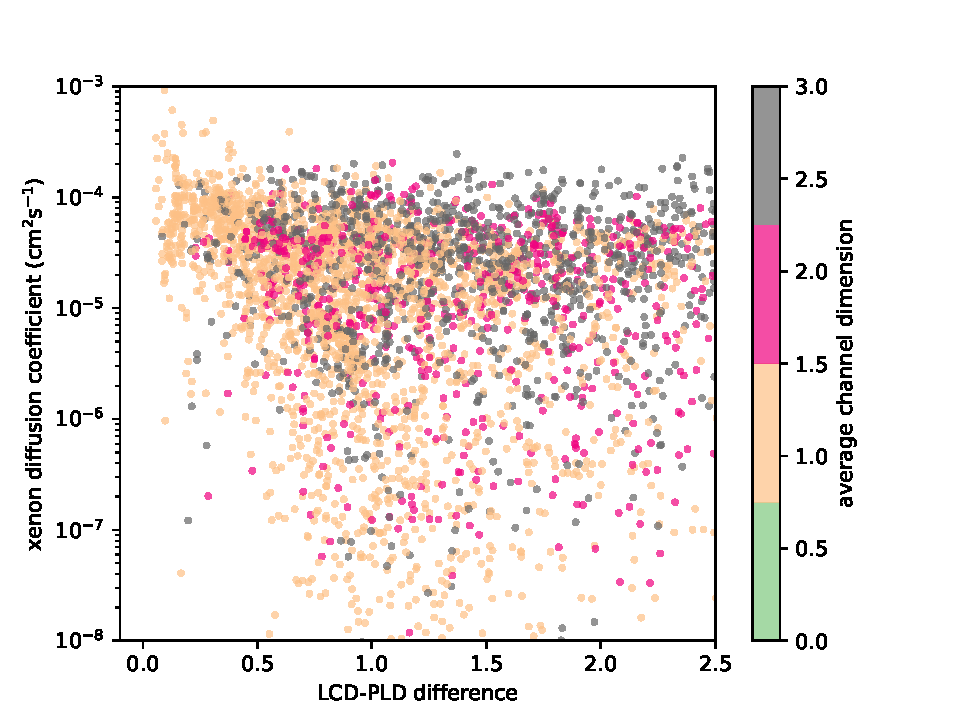
\includegraphics[width=\textwidth]{figures/5-diffusion/D_xe-poresize-chandim_all.pdf}
      \caption{All structures}\label{fgr:porediff_a}
  \end{subfigure}
  \hfill
  \begin{subfigure}[b]{0.32\textwidth}
      \centering
      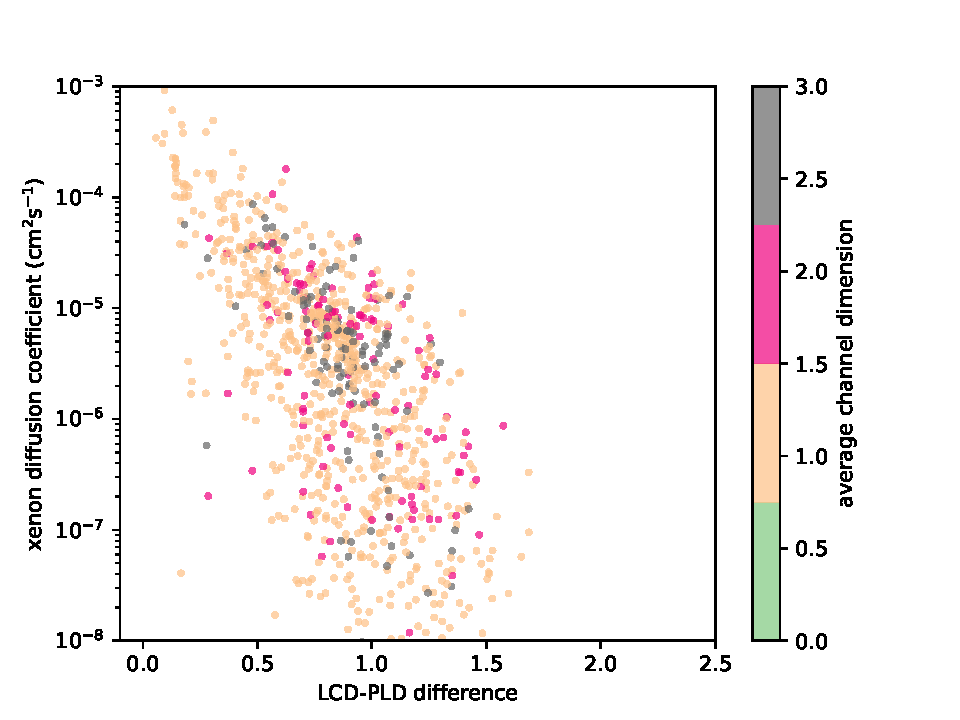
\includegraphics[width=\textwidth]{figures/5-diffusion/D_xe-poresize-chandim_LCDunder.pdf}
      \caption{LCD\ex{UFF}$<5.5$}\label{fgr:porediff_b}
  \end{subfigure}
  \hfill
  \begin{subfigure}[b]{0.32\textwidth}
      \centering
      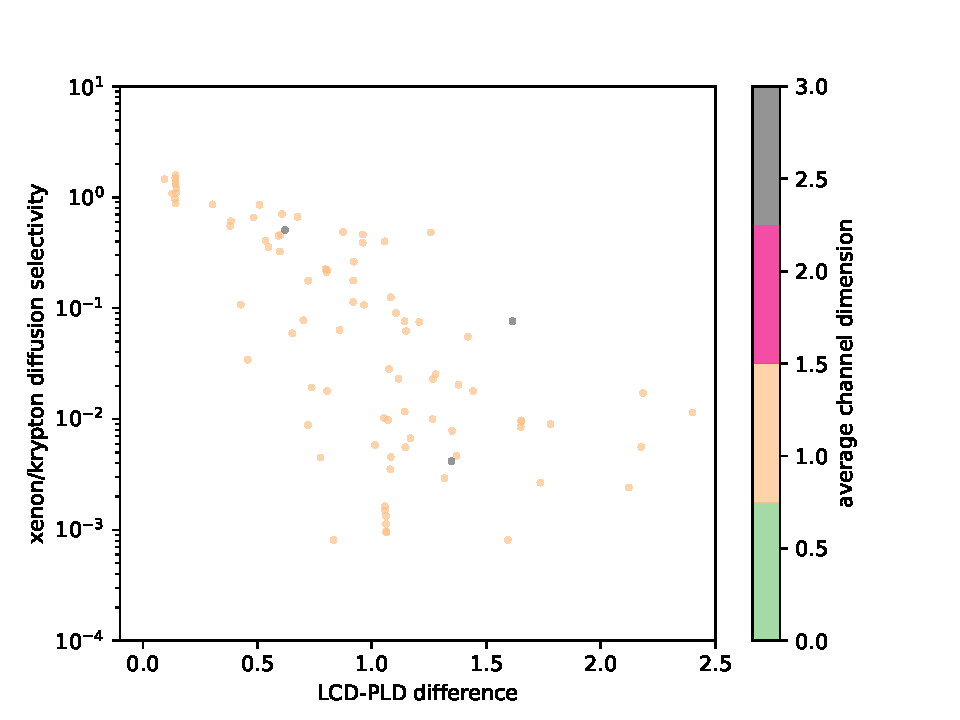
\includegraphics[width=\textwidth]{figures/5-diffusion/diff_D_xekr-poresize-chandim.pdf}
      \caption{$s\ex{Xe/Kr}_1>30$}\label{fgr:porediff_c}
  \end{subfigure}
     \caption{ Scatterplots of the diffusion coefficient compared to the LCD-PLD difference labeled using the channel dimension for all structures (a) and for structures with an LCD above \SI{5.5}{\angstrom} (b). On the subfigure (c), the scatterplot of the xenon/krypton diffusion selectivity compared to the LCD-PLD difference for the most selective structures ($s\ex{Xe/Kr}_1>30$). }\label{fgr:porediff}
\end{figure}

The highly selective materials displayed in Figure~\ref{fgr:porediff_c} are presented in Table~\ref{table:diff}. The negative linear relation between the LCD-PLD difference and the Xe/Kr diffusion selectivity or the Xe diffusion coefficient can be reaffirmed by examining the values in Table~\ref{table:diff} for materials with 1D channels (except \texttt{ADOGEH}). Two categories will be created to explore the tortuosity difference between these materials.

Materials with nanopores composed of pseudo-spherical cavities connected by cylindrical channels following a straight line are the first category, as shown in Figure~\ref{fgr:tube_cavities}. These channels would in fact have very low tortuosity if evaluated. For \texttt{TONBII}\todo{present it}, the very small LCD-PLD difference explains the relatively high diffusion selectivity near $1$. There is hardly any difference in the diffusion of xenon and krypton in the channels of this material. As the LCD value increases for similar PLD values, the diffusion selectivity of materials like \texttt{BAEDTA01} and \texttt{XUNSOQ}\todo{present them} decreases, as indicated in Table~\ref{table:diff}. This drop can be attributed to a lower xenon diffusion coefficient.

\begin{figure}[ht]
  \centering
  \begin{subfigure}[b]{0.32\textwidth}
      \centering
      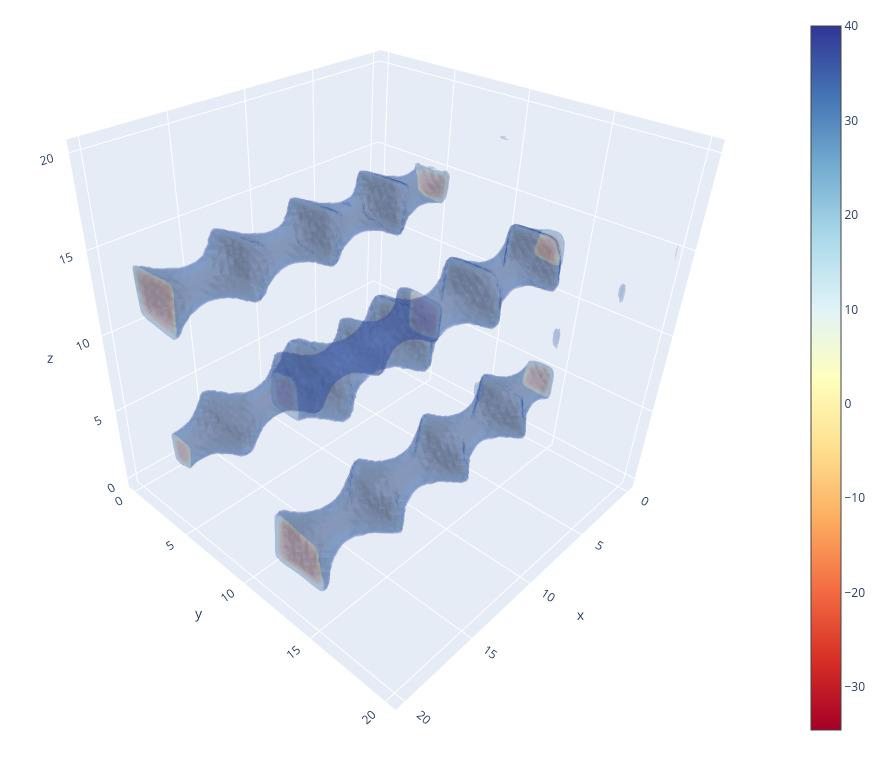
\includegraphics[width=\textwidth]{figures/5-diffusion/viz/XUNSOQ.jpg}
      \caption{\texttt{XUNSOQ}~\cite{Abrahams_2014}}\label{fgr:tube_cavities_a}
  \end{subfigure}
  \hfill
  \begin{subfigure}[b]{0.32\textwidth}
      \centering
      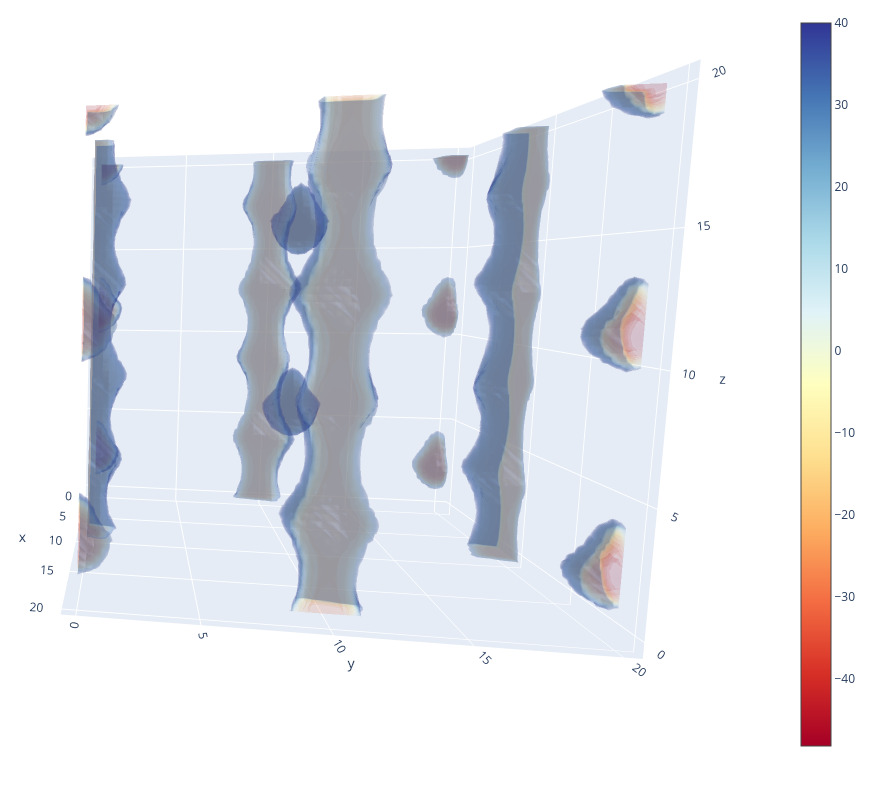
\includegraphics[width=\textwidth]{figures/5-diffusion/viz/BAEDTA01.jpg}
      \caption{\texttt{BAEDTA01}~\cite{Chen_2010}}\label{fgr:tube_cavities_b}
  \end{subfigure}
  \hfill
  \begin{subfigure}[b]{0.32\textwidth}
      \centering
      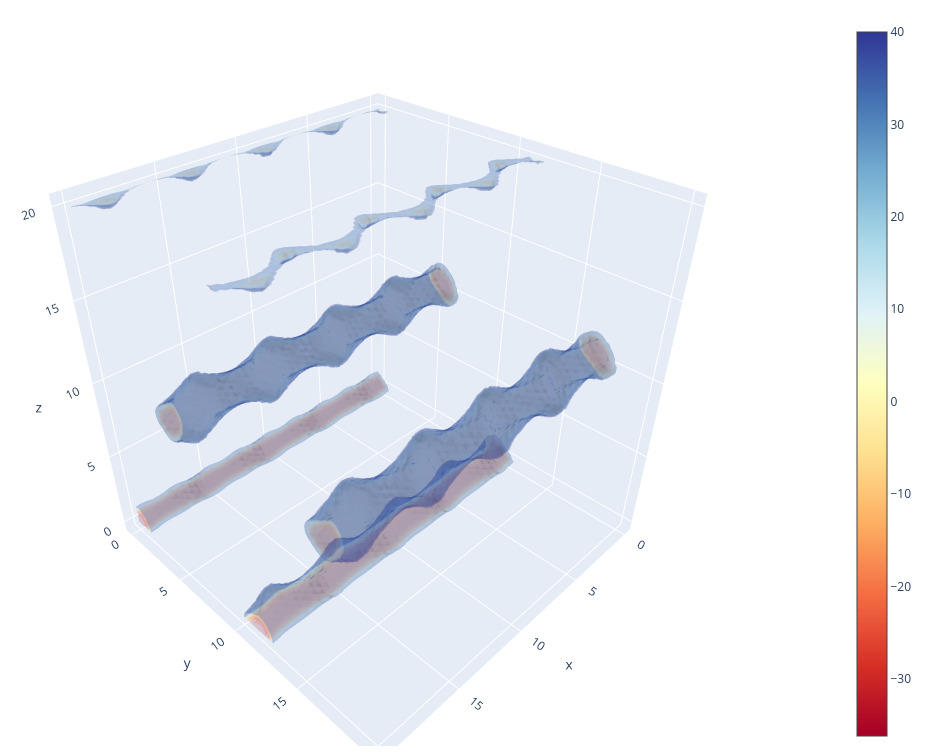
\includegraphics[width=\textwidth]{figures/5-diffusion/viz/TONBII.jpg}
      \caption{\texttt{TONBII}~\cite{Du_2010}}\label{fgr:tube_cavities_c}
  \end{subfigure}
     \caption{ 3D volume plot of the xenon interaction energy values inside materials with non-tortuous unidimensional channels calculated using an energy grid, as previously described.}\label{fgr:tube_cavities}
\end{figure}

Beyond the consideration of the pure diffusion properties, the relatively high adsorption selectivity coupled with minimal diffusion limitations make these materials intriguing for further study. The material \texttt{BAEDTA01}, which was previously discussed in relation to the selectivity drop caused by changes in pressure conditions, reveals the microscopic origins of this drop in Figure~\ref{fgr:tube_cavities_b}. The two distinct adsorption sites (one narrower than the other) can be clearly observed --- with the narrower site contributing to the extremely high selectivity at low pressures. The other materials, \texttt{TONBII} and \texttt{XUNSOQ}, maintain a relatively stable selectivity between low and ambient pressure cases. Compared to the \texttt{KAXQIL} structure identified in a previous high-throughput screening~\autocite{Simon_2015}, these materials exhibit higher diffusion coefficients and resolve the potential issue of diffusion limitation. However, the selectivity values of these materials are yet to be confirmed. While the value of the PLD is the primary factor explaining the lower diffusion coefficient of \texttt{KAXQIL}, the LCD-PLD difference can serve as a secondary variable to distinguish materials with similar PLD values but different diffusion coefficients.


Other materials, as seen in Figure~\ref{fgr:zigzag}, consist of channels that are much more tortuous than the previous type. They exhibit a "zigzag-like" shape. Quantifying the effect of tortuosity on the diffusion coefficient is challenging with the limited data available at this stage --- to achieve this, a comparison of highly similar materials (same chemical nature, same pore size) with differing tortuosity would be necessary. A theoretical perspective suggests that tortuosity typically has a negative impact on diffusion coefficients. For example, \texttt{VOHQIS} displays high degree of tortuosity, as shown in Figure~\ref{fgr:zigzag_a}, and its diffusion properties are not particularly high. However, it is difficult to disentangle the effects of pore size (significant difference between LCD and PLD) from the impact of tortuosity. A more quantitative approach is required to gain deeper insight into the diffusion process in nanoporous materials. 

\begin{figure}[ht]
  \centering
  \begin{subfigure}[b]{0.32\textwidth}
      \centering
      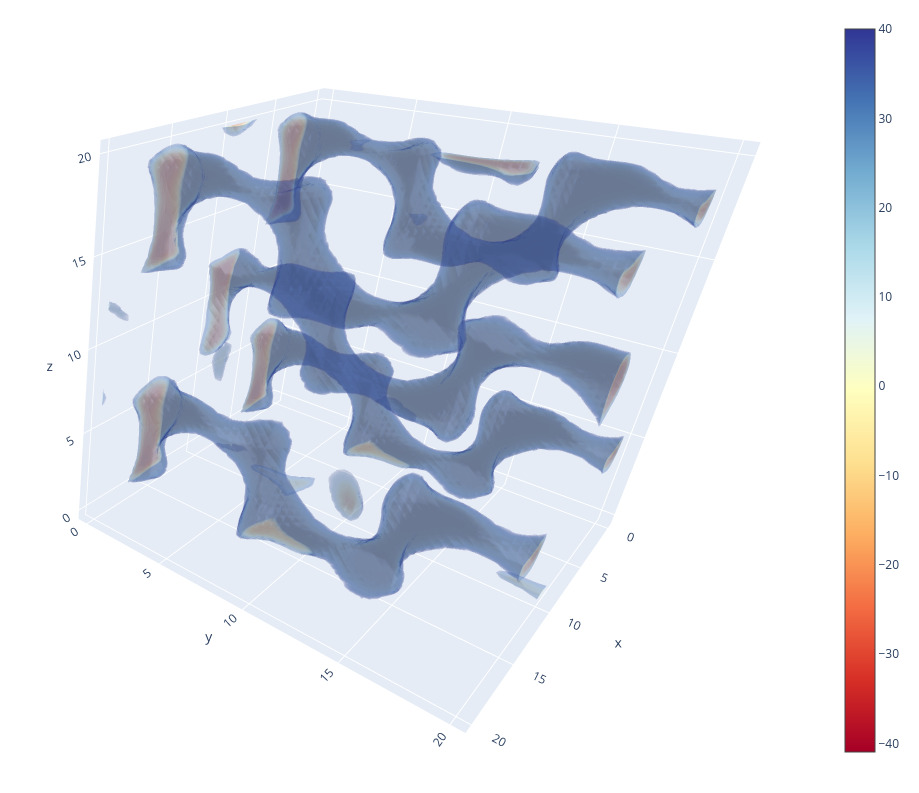
\includegraphics[width=\textwidth]{figures/5-diffusion/viz/VOHQIS.jpg}
      \caption{\texttt{VOHQIS}~\cite{Wragg_2001}}\label{fgr:zigzag_a}
  \end{subfigure}
  \hfill
  \begin{subfigure}[b]{0.32\textwidth}
      \centering
      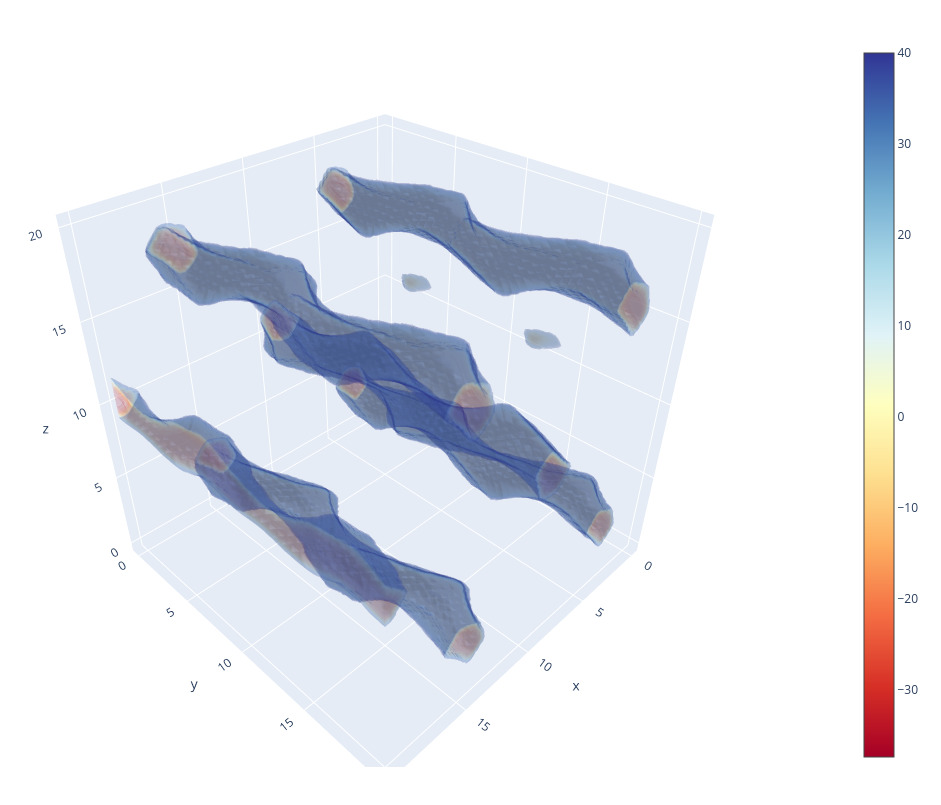
\includegraphics[width=\textwidth]{figures/5-diffusion/viz/GUMDEZ.jpg}
      \caption{\texttt{GUMDEZ}~\cite{Yin_2014}}\label{fgr:zigzag_b}
  \end{subfigure}
  \hfill
  \begin{subfigure}[b]{0.32\textwidth}
      \centering
      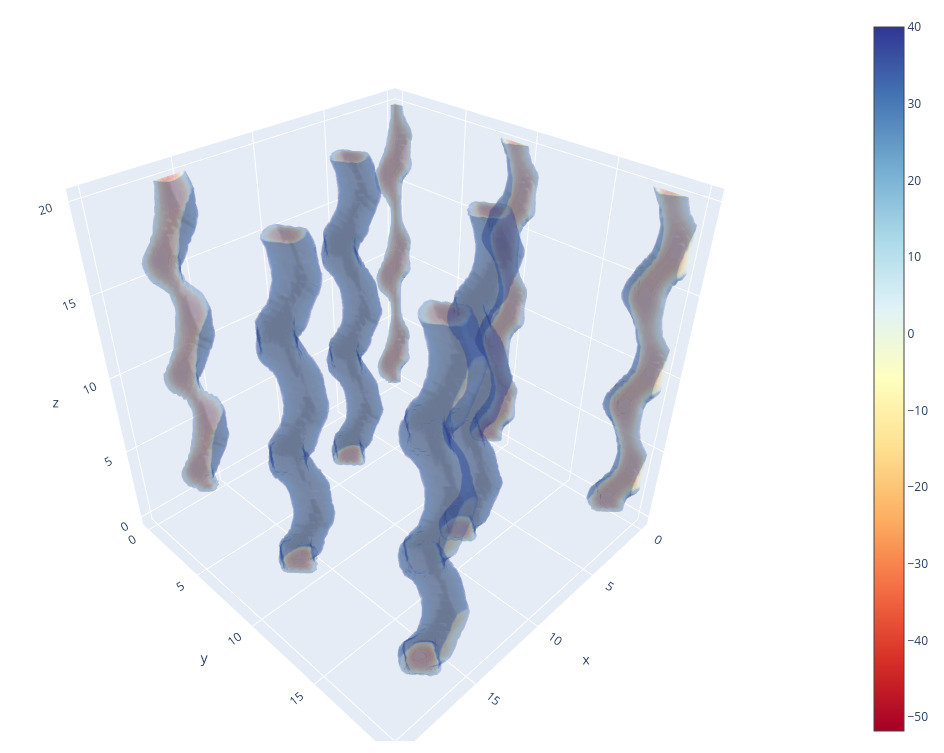
\includegraphics[width=\textwidth]{figures/5-diffusion/viz/MISQIQ.jpg}
      \caption{\texttt{MISQIQ}~\cite{Tong_2013}}\label{fgr:zigzag_c}
  \end{subfigure}
     \caption{ 3D volume plot of the xenon interaction energy values inside materials with tortuous unidimensional channels calculated using an energy grid as previously described.}\label{fgr:zigzag}
\end{figure}

A similar analysis to the previous materials with straight channels reveals similar findings for these more tortuous ones, which is not surprising as these materials are included in the correlation plot in Figure~\ref{fgr:porediff_c}. \texttt{GUMDEZ} is much less tortuous, as shown in Figure~\ref{fgr:zigzag_b}, but the difference in pore size is also smaller, resulting in a higher diffusion coefficient, which explains the good diffusion selectivity. This material also has significantly higher xenon uptake compared to more selective materials like \texttt{KAXQIL}, reflecting the uptake--selectivity as illustrated in Figure~\ref{fgr:sa}. Therefore, \texttt{GUMDEZ} and \texttt{QOZDOY} were previously identified in the literature by Chung et al.\autocite{Chung_2019} during the xenon/krypton separation screening conducted while introducing the CoRE MOF 2019 database. These materials were noted for their high xenon/krypton selectivity and substantially higher xenon uptake, which is a key metric for industrial separation processes --- it typically determines the amount of xenon retrieved per adsorption--desorption cycle. To improve the screening process, optimization of xenon uptake could be added alongside optimization of diffusion and selectivity properties. Fortuitously, this study identified materials such as \texttt{XUNSOQ}, \texttt{QOZDOY}, and \texttt{GUMDEZ} with good adsorption selectivity, diffusion selectivity, and xenon uptake that could be much more versatile than highly specialized materials like \texttt{KAXQIL}.

In summary, a screening of diffusion properties for xenon and krypton was conducted to complement the previous thermodynamic properties screening. Materials with a balanced combination of diffusion and adsorption selectivity values were identified, some of which exhibited very high Xe uptake, potentially enhancing the productivity of xenon separation processes by increasing separative capacity and facilitating rapid gas penetration within the material. This study further justifies the multivariate nature of the optimization problem when searching for suitable materials for xenon/krypton separation --- relying solely on a single variable is insufficient. The study provides a more comprehensive approach compared to existing studies (on other systems), highlighting the significance of kinetic effects in adsorption processes.\autocite{Stanton_2022} Further investigation is required to gain a better understanding of the relationship between diffusion properties, tortuosity, and each pore size effect. The next section will be dedicated to the development of faster methodologies for screening transport properties to scale up the screening process for larger databases. To achieve faster transport property screening, methods based on the transition state theory and machine learning prediction models were explored.

\section{Fast diffusion calculation algorithm}\label{sct:algo_diff}

To overcome the high computational demands of MD simulations, alternative methods were developed during this thesis to calculate the diffusion coefficient. One such method involves utilizing the transition state theory to generate MSD at larger timescales more efficiently. By applying a similar algorithm as in TuTraST, it becomes possible to address the initialization problem encountered in MD simulations when dealing with different channels in an automated screening process --- while it is feasible to manually place a particle in a specific initial state, achieving this within a screening process can be challenging. Although the implementation of the C++ algorithm that directly reproduces diffusion coefficients through a rejection-free lattice kinetic Monte Carlo algorithm is not yet complete, the initial implementation was employed to calculate maximum energy barriers within a material. These energy values provide additional information alongside PLD values for predicting diffusion coefficients, and a ML model was trained to predict diffusion coefficients much faster than the current MD method.

\subsection{Code based on the TuTraST algorithm}

The GrAED algorithm, as presented in section~\ref{sct:grid}, was employed to calculate the xenon interaction energy with the material at each non-overlapping point of the symmetry-aware grid. This energy grid enables the identification of different channels, adsorption pores, and the transition surface that separates them.

A slight modification was made to the approach previously described in section~\ref{sct:tutrast} and adopted by Mace et al.,\ to identify the three main components of the lattice Monte Carlo approach. Rather than detecting the channels on the fly, the decision was made to pre-detect the channels to restrict the cluster growth to a specific channel. This approach aims to reduce the computation time required during the clustering step by simulating only one representative channel out of all the potentially equivalent channels --- due to the high level of symmetry, multiple equivalent channels typically exist within a single unit cell, as illustrated in Figures~\ref{fgr:tube_cavities} and~\ref{fgr:zigzag}.

To identify the various channels, a breadth-first search algorithm was utilized to find all connected grid points with an energy below a specified threshold value ($E\e{cutoff}$). The determination of connections between rhomboidal grid voxels (same angles as the unit cell) was based on voxel faces, resulting in six nearest neighbors. Additional connections from the eight edges were considered, totaling 14 nearest neighbors. Including the vertices would yield 26 nearest neighbors. However, for simplicity, only the six primary connections were employed. The breadth-first search algorithm for a grid system is relatively straightforward:

All the points of the grid are iterated over:
  \begin{enumerate}
    \item If the point has not been visited and its energy is below the threshold, it is added to the cluster and a queue. A search can be initiated to identify all connected neighbors.
    \item Each (face-connected) neighbor of the point is tested and added to the cluster and a queue if it has not been visited and its energy is below the threshold.
    \item The process is repeated for all elements in the queue until the queue becomes empty. This yields all grid points connected to the initial point at the end. The main loop then restarts, and the search is only initiated if an unvisited point is encountered.
  \end{enumerate}
The breadth-first search ends with clusters of connected points that are below the energy threshold. Each of these clusters can be tested to see if they represent channels (connected all the way through a periodic boundary).

Having identified well-defined channels and pockets within the nanoporous material, symmetrically equivalent channels can be identified using the symmetric grid explained in section~\ref{sct:grid}. Typically, only a few unique channels (usually fewer than three) remain, which can be used for basin-cluster growth and the detection of TS surfaces that separate these basins.

Next, the algorithm proceeds by iterating over energy values (with a step size of \SI{1}{\kJ\per\mole} used in the original paper) and growing the cluster layer by layer. An improvement is introduced at this stage, wherein the previous search algorithm is employed to efficiently count the number of clusters within a given channel. If this number changes, it indicates that some clusters have merged. When the energy gap is sufficiently large, TS surfaces can be detected using a layer-by-layer growth approach within a small energy range ($[E,\ E+\delta E]$) to generate a smoother surface.

The current development of this detection algorithm is at its final stage, as it was temporarily paused to focus on analyzing the barrier energies calculated from a modified version of the initial implementation, which will be detailed in the following discussions. The detection of transition surfaces will be further explored in the following chapter, with an attempt to implement a more optimized version that avoids the computationally expensive layer-by-layer growth.

\subsection{Calculation of a diffusion activation energy}

As the aim of this study is to only determine the activation energy, the more computationally demanding TS detection and kinetic Monte Carlo steps can be skipped. Instead, the breadth-first search algorithm is employed to label different connected components within a given channel between $E\e{min}$ and $E\e{min}+i\delta E$ (at the $i$\ex{th} iteration). By monitoring changes in the number of connected components between two energy values, the code automatically detects the energy $E\e{trans}$ at which components reconnect and form a channel (allowing diffusion from one boundary to another). The activation energy $E\e{a}$ is then calculated as the difference between the calculated transition state energy $E\e{trans}$ and the minimum energy $E\e{min}$ within the channel.

In the case of \texttt{KAXQIL}, barrier detection was performed using an energy step $\delta E$ of \SI{0.3}{\kJ\per\mol}. A single symmetrically unique type of channel was identified in \texttt{KAXQIL}, with a minimal energy of $-44.3$~\si{\kJ\per\mole} --- the various channels shown in Figure~\ref{fgr:KAXQIL_channel} are all symmetrically equivalent. The code detected a single merge that resulted in a fully connected component within the channel. This merging occurred at an energy of $-25.7$~\si{\kJ\per\mole} (as depicted in Figure~\ref{fgr:KAXQIL_23}), indicating that the estimated activation energy is $18.6$~\si{\kJ\per\mole} with an error of \SI{0.3}{\kJ\per\mole} (due to the energy step used).

\begin{figure}[ht]
  \centering
  \begin{subfigure}[b]{0.32\textwidth}
    \centering
    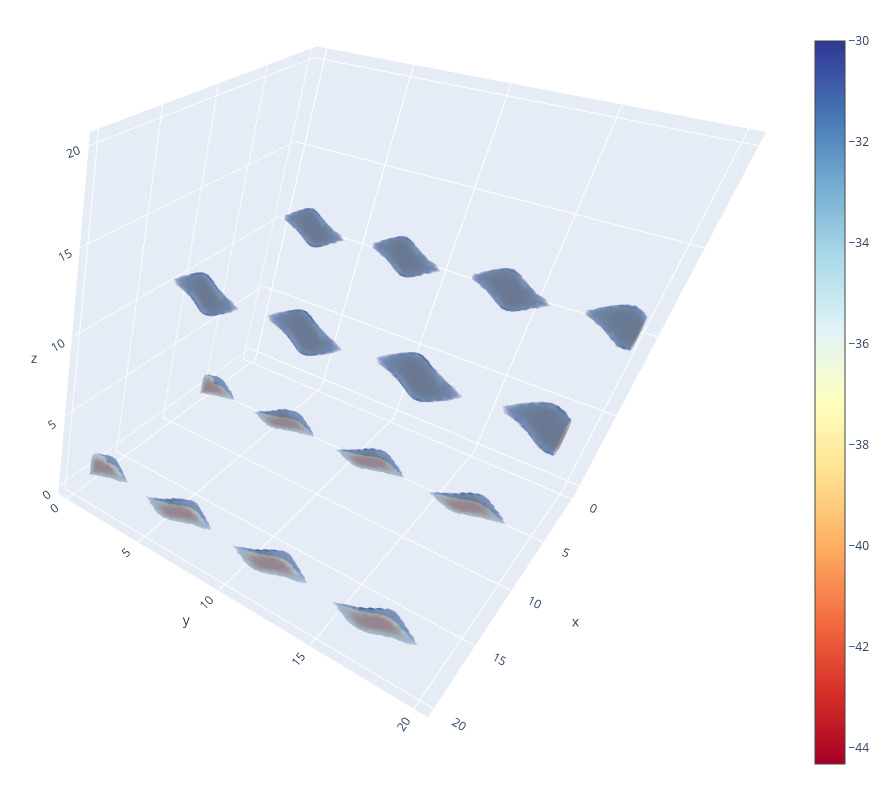
\includegraphics[width=\textwidth]{figures/5-diffusion/KAXQIL_30.jpg}
    \caption{$E\e{max}<-30$}~\si{\kJ\per\mole}\label{fgr:KAXQIL_30}
  \end{subfigure}
  \hfill
  \begin{subfigure}[b]{0.32\textwidth}
    \centering
    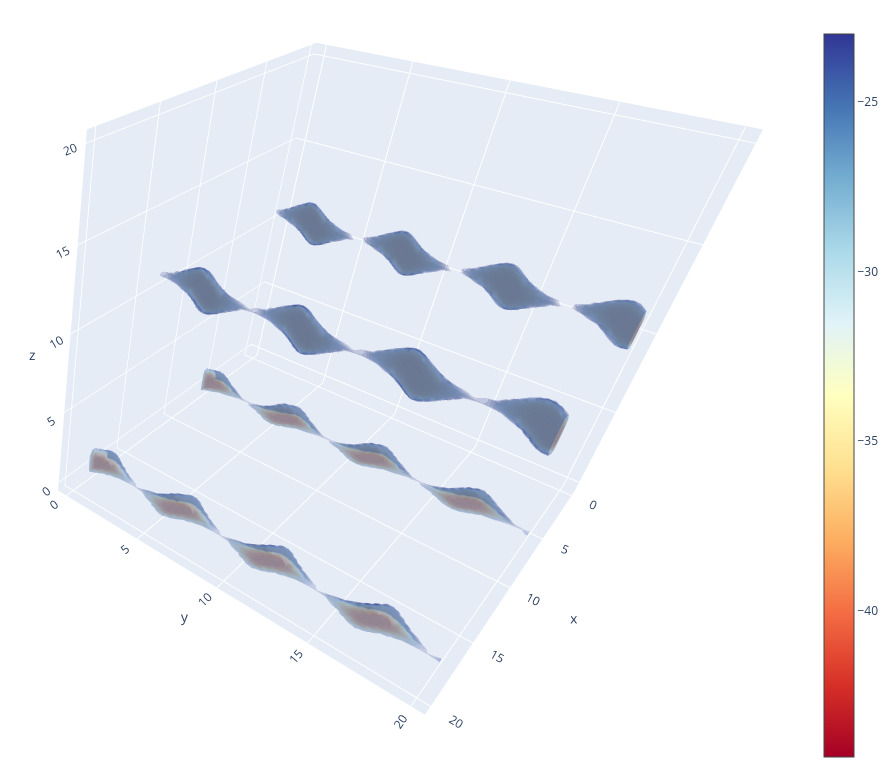
\includegraphics[width=\textwidth]{figures/5-diffusion/KAXQIL_23.jpg}
    \caption{$E\e{max}<-23$}~\si{\kJ\per\mole}\label{fgr:KAXQIL_23}
  \end{subfigure}
  \hfill
  \begin{subfigure}[b]{0.32\textwidth}
      \centering
      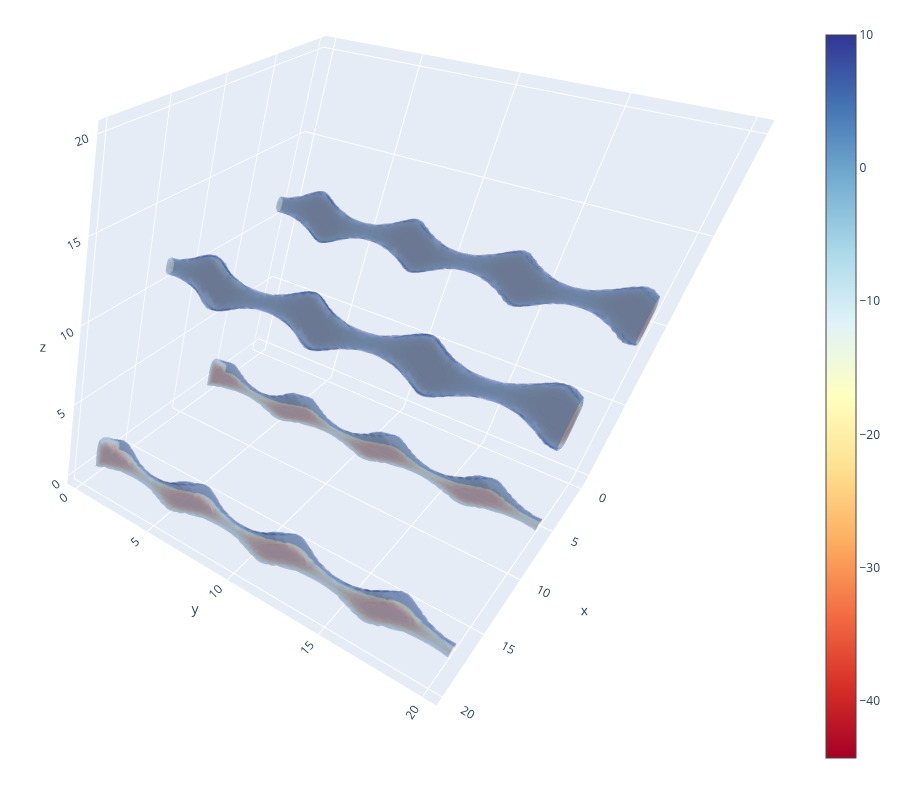
\includegraphics[width=\textwidth]{figures/5-diffusion/KAXQIL_10.jpg}
      \caption{$E\e{max}<10$}~\si{\kJ\per\mole}\label{fgr:KAXQIL_channel}
  \end{subfigure}
    \caption{ 3D visualization of channels within \texttt{KAXQIL} using different energy thresholds $E\e{max}$. Depending on the maximum value of energy allowed, the channel is either composed of unconnected basins (a), or they are fully connected (b) and (c). This illustrates the principle of the energy barrier detection. }\label{fgr:KAXQIL_channels}
\end{figure}

In this case of one unique merge of a unidimensional channel, the method demonstrates strong performance, and it becomes possible to associate the activation energy with a diffusion rate $k\e{diff}$ using the Arrhenius equation:
\begin{equation}
  k\e{diff} = A \exp\left(-\frac{E\e{a}}{k\e{B}T}\right)
\end{equation}
where $A$ is a prefactor that depends on the temperature and system (adsorbate, adsorbent). This is a simplified version of the equations~\ref{eq:trans_rate_path} and~\ref{eq:trans_rate} used in transition state theory-based methods. In the case of a unidimensional channel with a single possible transition, the diffusion coefficient is directly associated with the diffusion rate. The problem can be reduced to a unidimensional random walk with a given transition probability, and the diffusion coefficient is given by $D=0.5k\e{diff}L^2$ where $L$ is the distance between two basins (in one dimension). In this special case, there exists a direct relationship between the diffusion coefficient and the activation energy such that $\log(D)\propto E\e{a}$. For more complex systems than \texttt{KAXQIL}, these methods may not yield satisfactory results. 

Describing the case of multistep diffusion is particularly challenging. For example, a particle can cross a series of lower barriers instead of encountering the highest energy gap as calculated by the method of this work, as illustrated in Figure~\ref{fgr:TS_problem}. In such cases, the relevant activation energy is the maximum value among these two activation energies. Even when considering the maximum activation energy, if the values are similar, this approximation may not be justified. Both transitions would influence the diffusion process. This approximation holds true only when one of the activation energies is significantly larger than the other ($E\e{a}^1 \gg E\e{a}^2$).

\begin{figure}[ht]
  \centering
    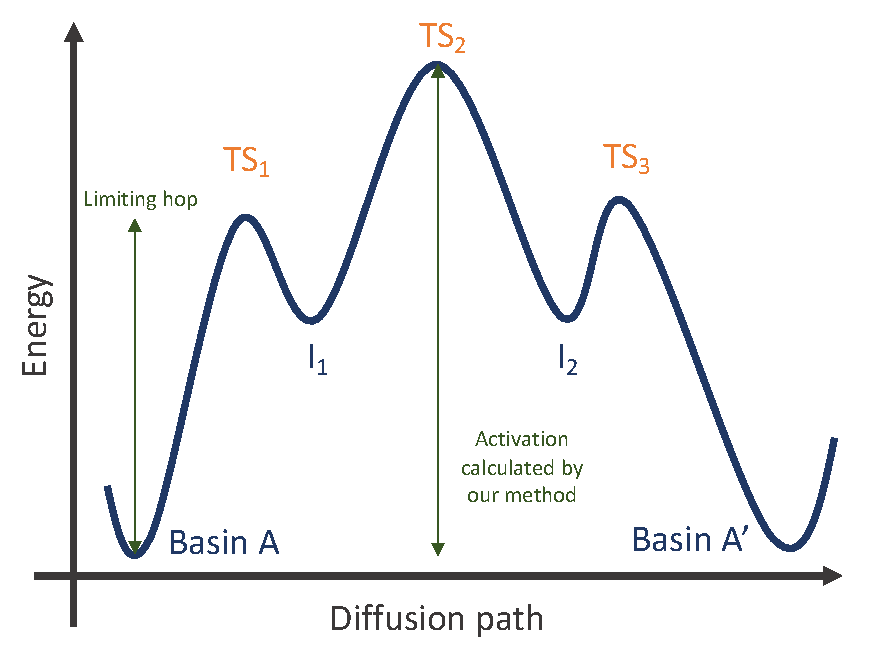
\includegraphics[width=0.6\textwidth]{figures/5-diffusion/Diffusion_TS.pdf}
    \caption{Multistep diffusion from a basin A to a basin A'. The diffusion process is modeled by transition states TS$_1$, TS$_2$ and TS$_3$ and intermediate steps I$_1$ and I$_2$. In this particular case, there is a difference between the real limiting activation energy and the activation energy calculated by the simplified method. }\label{fgr:TS_problem}
\end{figure}

To improve this approach, intermediate transition state energy values can be detected by examining the change in the number of clusters, for instance. However, it remains difficult to determine which combinations of energy differences are relevant, and a more detailed investigation of the location of these transition states is required, which brings the discussion back to the initial issue of TS surface detection that has remained on standby. Despite these limitations, this quickly measurable activation energy can be employed as a proxy for the diffusion coefficient.
The subsequent discussion will focus on the relationship between this approximated activation energy value and the diffusion coefficients. This new diffusion descriptor can later be incorporated into prediction models as a complementary feature to the PLD, providing a more comprehensive picture of the diffusion process.

\subsection{Relation of this activation energy to the diffusion}

\todo{HERE}
The xenon diffusion activation energy was calculated for all the 5,125 structures selected for the xenon diffusion coefficient screening presented in section~\ref{sct:xenon_diff_screen}. An energy step of $\delta E$ of \SI{0.1}{\kJ\per\mol} was employed during the energy loop to determine the minimal energy barrier for each unique channel in the material. Subsequently, an activation energy can be derived and compared to the diffusion coefficients. To avoid any potential noise arising from the MD simulation initialization problem, materials with significantly different energy barrier values from one channel to another (standard deviation of energy barrier values higher than \SI{1}{\kJ\per\mol}) were excluded. These materials accounted for only 145 out of the total 5,125 materials.


\begin{figure}[ht]
  \centering
  \begin{subfigure}[b]{0.48\textwidth}
    \centering
    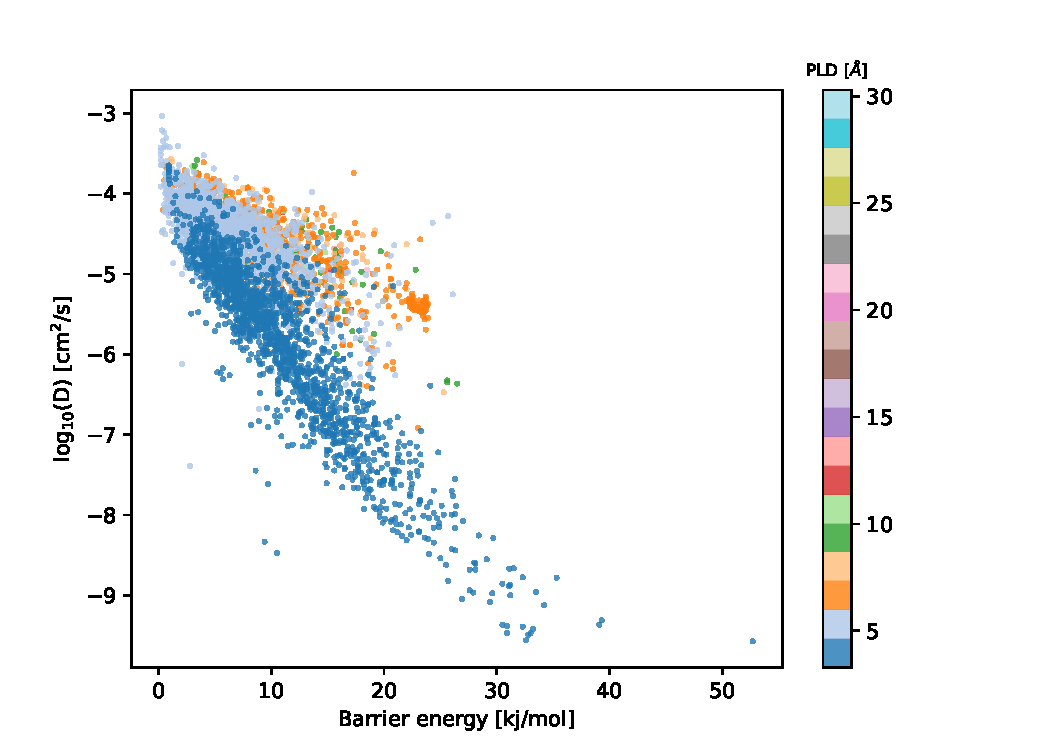
\includegraphics[width=\textwidth]{figures/5-diffusion/difflog_barrier_Df_uff.pdf}
    \caption{All structures}\label{fgr:barrier_diffusion_a}
\end{subfigure}
  \hfill
  \begin{subfigure}[b]{0.48\textwidth}
      \centering
      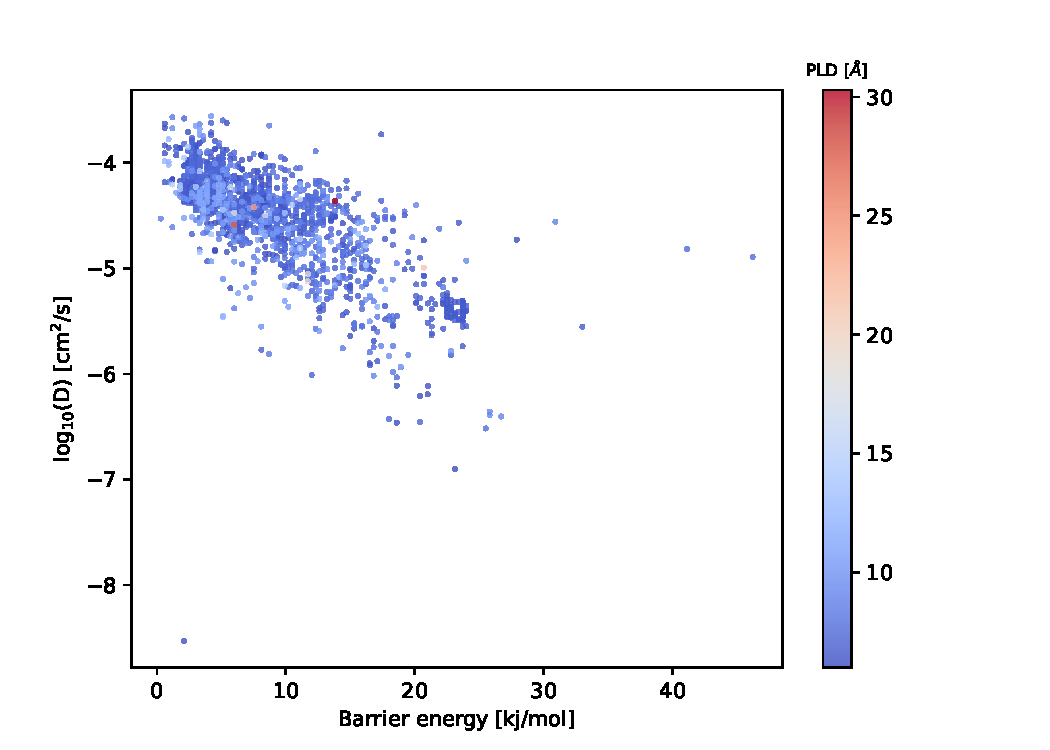
\includegraphics[width=\textwidth]{figures/5-diffusion/difflog_barrier_Df_uff_2.pdf}
      \caption{PLD over \SI{6}{\angstrom}}\label{fgr:barrier_diffusion_b}
  \end{subfigure}
    \caption{ Scatterplots of the $\log_{10}$ of the diffusion coefficient (in \si{\square\cm\per\s}) compared to the diffusion activation energy $E\e{a}$ in \si{\kJ\per\mol} (a) for all structures  and (b) for the structures with a PLD above \SI{6}{\angstrom}. For all structures, the Pearson correlation coefficient is equal to $-0.77$, whereas for the restriction to structures with a PLD below \SI{6}{\angstrom} this correlation is stronger with a Pearson coefficient of $-0.85$. For structures with a PLD above \SI{6}{\angstrom}, this coefficient decreases to reach $-0.74$.}\label{fgr:barrier_diffusion}
\end{figure}

As shown in Figure~\ref{fgr:barrier_diffusion_a}, the activation energy is correlated with the diffusion coefficient for xenon. A stronger correlation is observed for points with a PLD around \SI{4.5}{\angstrom}, while for PLD values exceeding \SI{6}{\angstrom}, the correlation appears to be weaker compared to smaller PLD values, as illustrated in Figure~\ref{fgr:barrier_diffusion_b}

This correlation between the energy barrier and the diffusion coefficient is confirmed in Figure~\ref{fgr:diff_pld_barrier}. The points are labeled according to their energy barrier value, and the highest energy barrier points tend to be concentrated among lower diffusion coefficient values. However, a few points with very high energy barriers are also observed for diffusion coefficients that are quite low. There are two such points detectable with the naked eye. 

\begin{figure}[ht]
  \centering
    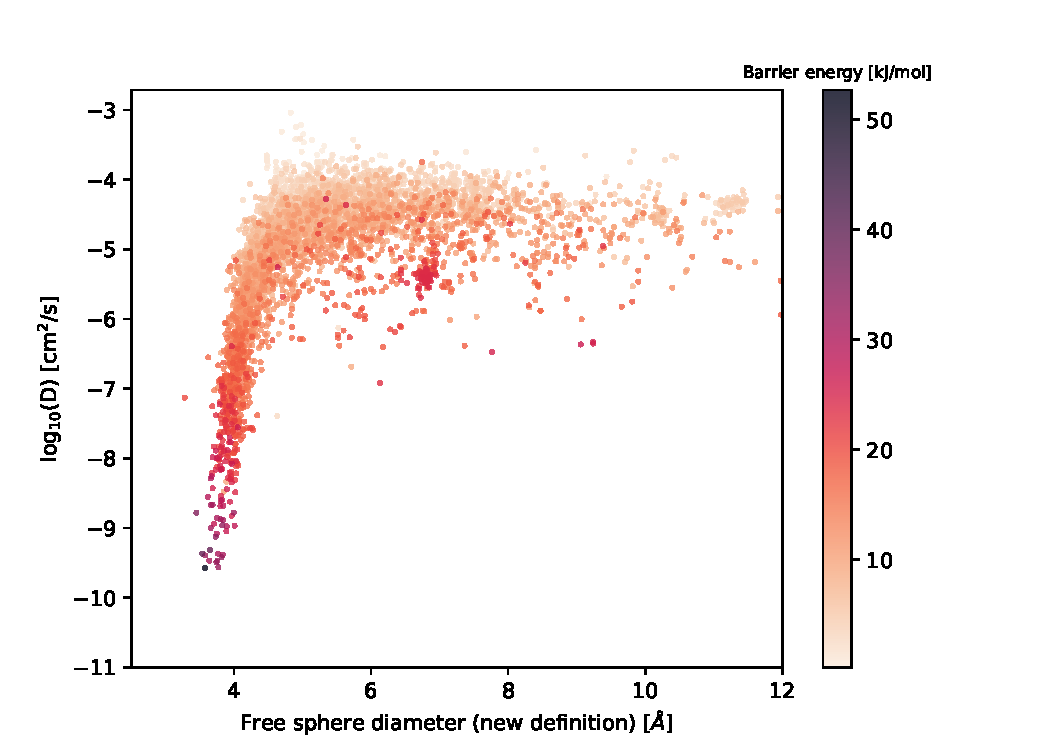
\includegraphics[width=0.6\textwidth]{figures/5-diffusion/difflog_Df-uff298K_barrier.pdf}
    \caption{ Scatterplot of the $\log_{10}$ of the diffusion coefficient in \si{\square\cm\per\s} as a function of the PLD values and labeled by the barrier activation energy. The higher barriers seem to correspond to lower diffusion coefficients, thus echoing the correlation observed in the previous figure~\ref{fgr:barrier_diffusion}.}\label{fgr:diff_pld_barrier}
\end{figure}

This barrier activation energy descriptor completes the description of the diffusion coefficient given by PLD values. As discussed in the dedicated section, PLD values cannot distinguish between structures over \SI{6}{\angstrom} in the ``plateau'', and the difference in diffusion coefficient values was considered as noise in the previous analysis. However, Figure~\ref{fgr:diff_pld_barrier} reveals that higher values of barrier energies are associated with lower diffusion coefficients within the plateau range, thereby explaining the variations in diffusion coefficient within the plateau based on the activation barrier values.
Although the correlation is not perfect, this barrier descriptor provides better insights into this uncharted area of PLD values above \SI{6}{\angstrom}, which cannot be explained by simple geometric considerations. The barrier activation energy value sheds light on the chemical nature of the diffusion barrier that needs to be overcome.

In the final section of this chapter, the combination of geometrical descriptors with this energy barrier will be employed to train a machine learning model, following the same approach as in the previous Chapter 4. The energy barrier and PLD values, the highest correlated descriptors, will play a prominent role in the final ML model. This model can then be utilized to evaluate the diffusion coefficient of xenon in other materials, offering a significantly faster alternative to MD simulations.

\subsection{ML prediction model}

Calculating diffusion coefficients is an extremely time-consuming process, complicated by various challenges in the final fitting procedure. Out of the initial 6,525 structures, over a thousand were lost, resulting in a success rate of approximately 79\%, mainly due to either insufficient time for obtaining a usable MSD or MSD that describe non-diffusional regimes. By utilizing an unconventionally higher time step, the time required to investigate the diffusion regime could be reduced to just a couple of days per structure. Compared to the \SI{12}{seconds} required for energy barrier calculations with an energy step of \SI{0.1}{\kJ\per\mol}, and the few minutes required to run Zeo++, the MD method is extremely slow. Even under highly optimistic assumptions for MD simulations, the comparison is essentially between 24 hours and at most 10 minutes per structure, which corresponds to an approximate speedup of 150-fold (though, in reality, it is much higher). However, the relationships between energy barrier, PLD, and diffusion coefficient remain unclear --- the Arrhenius law generalizes limited consideration of the weak correlation shown in Figure~\ref{fgr:barrier_diffusion_a}. The aim of the ML model is to establish this relationship and achieve accurate predictions while significantly reducing the time required for predicting the diffusion coefficient of future selective materials.


\begin{table}[ht]
  \setlength{\extrarowheight}{1pt}
  \centering
  \begin{tabular}{|l|c|m{8cm}|}
  \hline
    Feature name  &  Symbol   &   Description\\
  \hline
      "Framework Mass (g/mol)" &   $M_f$ &   Molar mass of the framework material considered  \\
      "Framework Density (kg/m\^3)" &   $\rho_f$ &   Mass density of the framework material considered  \\
      "ASA\_m2/cm3\_1.2" &   SA &   Surface area accessible to a \SI{1.2}{\angstrom} radius probe in \si{\square\m\per\cubic\cm}  \\
      "PO\_VF\_2.0" &  VF $\tfrac{V\e{pore}}{V\e{tot}}$ &  The void fraction or the ratio of the pore volume occupied by a \SI{2}{\angstrom} radius probe over the total material volume  \\
      "D\_f\_vdw\_uff298" &   PLD or $D_f$  &   Pore limiting diameter of the largest free sphere diameter calculated using the UFF dependent definition  \\
      "D\_if\_vdw\_uff298" &   LCD or $D_{if}$ &   The largest included free sphere diameter in a free diffusion path calculated using the UFF dependent definition  \\
      "Adsorption\_enthalpy" &   $\Delta\e{ads}H_0\ex{Xe}(\text{channel})$  &   Xenon adsorption enthalpy within a channel calculated using the barrier algorithm  \\
      "barrier\_kjmol" &   $E\e{a}$  &   difference between transition state energy $E\e{trans}$ and the minimal energy $E\e{a}$ within a channel \\
      "delta\_LCD\_PLD" &   LCD$-$PLD  &   difference between the LCD and PLD values \\
      "1D\_chan" &  $\mathbb{1}\e{1D}$   &   categorical feature: 1 if there is a unidimensional channel, 0 else \\
      "2D\_chan" &  $\mathbb{1}\e{2D}$   &   categorical feature: 1 if there is a bidimensional channel, 0 else \\
      "3D\_chan" &  $\mathbb{1}\e{3D}$   &   categorical feature: 1 if there is a tridimensional channel, 0 else \\
    \hline
  \end{tabular}
  \caption{ Features used in the ML model for diffusion coefficient prediction. }\label{Table:feat_diff}
\end{table}

The ML model was trained using {80\%} of the 4,873 structures that survived all the different imposed filters. A total of 12 descriptors described in Table\ref{Table:feat_diff} were employed to train the model. The hyperparameters of the XGBoost model were determined using a similar approach as in Chapter 4, and the following values were utilized:

\begin{lstlisting}[language=Python]
  optimal_params = {
      'objective': 'reg:squarederror',
      'n_estimators': 1500,
      'max_depth': 4,
      'colsample_bytree': 1,
      'colsample_bylevel': 0.75,
      'subsample': 0.75,
      'alpha': 0.6,
      'lambda': 1,
      'learning_rate': 0.04,
    }
\end{lstlisting}

With this parameterization, this ML model predicts the $\log_{10}$ of the diffusion coefficient (\si{\square\cm\per\s}) with a root mean square error of $0.26$ on the test set and a mean absolute error of $0.18$. This implies that the exponent $\alpha$ is known with an error of approximately $0.2$ when expressing the diffusion coefficient as $D = 10^{\alpha}$. For comparison, the previous ML model for thermodynamic selectivity predicts the $\log_{10}$ of selectivity with an error of about $0.07$. It is important to note that the goal here is not to predict the exact values of the diffusion coefficient due to the inherent noise the values generated by MD simulation (about {20\% relative error for \texttt{KAXQIL}}). Instead, the objective is to determine the order of magnitude of the diffusion coefficient. The proposed model achieves this objective effectively, as illustrated in Figure~\ref{fgr:diffusion_pred}, where the predicted diffusion coefficient aligns closely with the true values when represented on a log scale.


\begin{figure}[ht]
  \centering
  \begin{subfigure}[b]{0.48\textwidth}
    \centering
    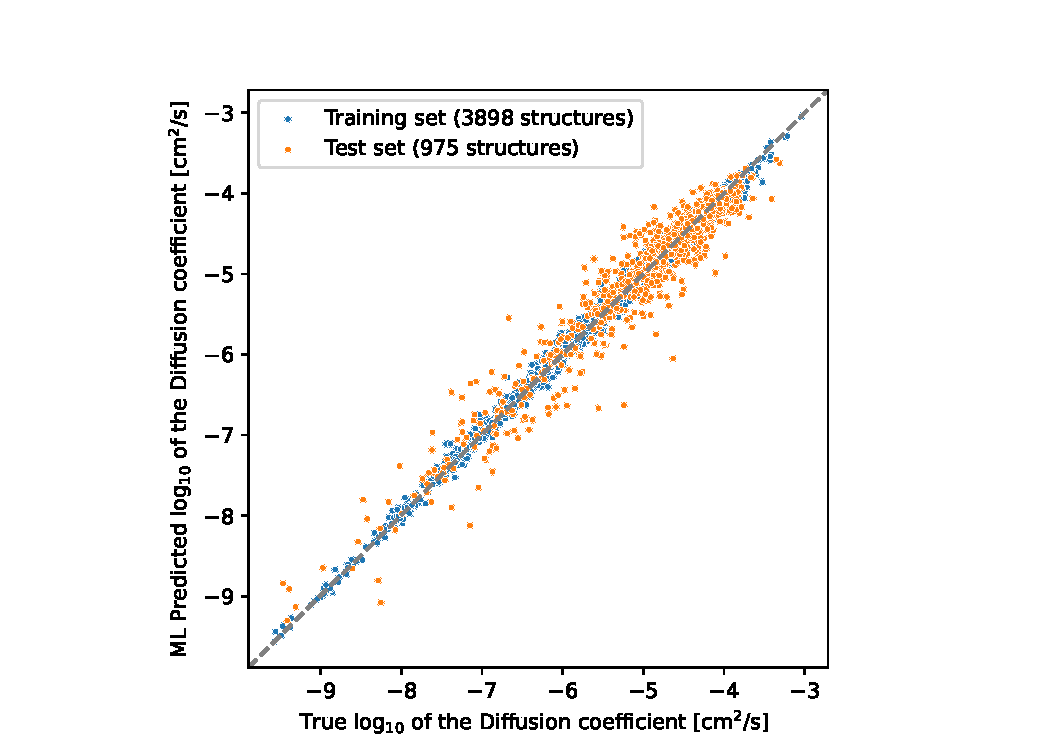
\includegraphics[width=\textwidth]{figures/5-diffusion/diffusion_prediction.pdf}
  \caption{Prediction result}\label{fgr:diffusion_pred}
  \end{subfigure}
  \begin{subfigure}[b]{0.48\textwidth}
    \centering
    \includegraphics[width=\textwidth]{figures/5-diffusion/training_curve.pdf}
    \caption{Training curve}\label{fgr:training_curve_diff}
  \end{subfigure}
    \caption{ (a) Comparison of the $\log_{10}$ of the diffusion coefficient predicted by an ML model and the true values. (b) Root mean squared errors on the same test set (20\% of all data) as a function of the fraction of the training set used to train smaller models. The error decreases as the amount of data increases and seems to stabilize near $0.25$. }
\end{figure}

The training curve (Figure~\ref{fgr:training_curve_diff}) was examined to assess whether the model had sufficient training data or required additional data. As the amount of training data increased, the error converged to $0.25$, indicating that no further data was necessary for training the model. However, it is conceivable to train a similar model using less data (50\% instead of 80\% of the total data could probably suffice to train a similar model).

\begin{figure}[ht]
  \centering
  \includegraphics[width=0.6\textwidth]{figures/5-diffusion/Diff_Feature_importance_shapbased.pdf}
  \caption{ Feature importance determined using the average of the absolute Shapley values for each feature based on every training data. An influential feature would have a very high average absolute SHAP value. The features are detailed in Table~\ref{Table:feat_diff}. }\label{fgr:feat_imp_diff}
\end{figure}

The ML model was interpreted using the SHAP algorithms discussed in the previous chapter. As expected, the most important features were found to be the PLD and the barrier activation energy, as demonstrated in the previous section. The void fraction also appeared to play a non-negligible role.

To unravel the relationship between these features and the target diffusion coefficient, partial dependence plots (PDPs) were examined for these features shown in Figure~\ref{fgr:pdp_selection_diff}. 

The PLD has a contribution similar to that described in section~\ref{sct:xenon_diff_screen}. A linear contribution was observed when the PLD values were below \SI{6}{\angstrom}, followed by a constant contribution for PLD values above this threshold. The activation energy showed a negative correlation with the log of the diffusion coefficient, which explained the linear contribution observed in the dependence plot.

The model also revealed less obvious contributions. Figure~\ref{fgr:diff_sa_vf} indicates that no clear relationships can be inferred between surface areas or void fractions and the diffusion coefficient. These factors played a more secondary role, slightly adjusting the obtained values with contributions of the order of $0.2$. For instance, the model identifies a positive relation between the void fraction and the contribution to the diffusion coefficient, which aligns with the physical understanding that lower void fractions correspond to lower diffusion rates within the material, assuming other parameters are equal. Conversely, larger surface areas imply more interaction with the pore walls, which slows down the diffusion of particles. Regarding the LCD, the LCD-PLD difference, xenon adsorption enthalpy, framework's mass, and density, no clear contribution patterns were observed. This may be attributed the fact that the previous features account for a substantial portion of the contribution due to the correlation between all these features.

\begin{figure}[ht]
  \centering
    \includegraphics[width=0.32\linewidth]{figures/5-diffusion/PDP/D_f_vdw_uff298.pdf}
    \includegraphics[width=0.32\linewidth]{figures/5-diffusion/PDP/barrier_kjmol.pdf}
    \includegraphics[width=0.32\linewidth]{figures/5-diffusion/PDP/PO_VF_2.0.pdf}
    \includegraphics[width=0.32\linewidth]{figures/5-diffusion/PDP/ASA_m2_cm3_1.2.pdf}
    \includegraphics[width=0.32\linewidth]{figures/5-diffusion/PDP/D_if_vdw_uff298.pdf}
    \includegraphics[width=0.32\linewidth]{figures/5-diffusion/PDP/Framework Density (kg_m^3).pdf}
    \includegraphics[width=0.32\linewidth]{figures/5-diffusion/PDP/Adsorption_enthalpy.pdf}
    \includegraphics[width=0.32\linewidth]{figures/5-diffusion/PDP/Framework Mass (g_mol).pdf}
    \includegraphics[width=0.32\linewidth]{figures/5-diffusion/PDP/delta_LCD_PLD.pdf}
    \includegraphics[width=0.32\linewidth]{figures/5-diffusion/PDP/1D_chan.pdf}
    \includegraphics[width=0.32\linewidth]{figures/5-diffusion/PDP/2D_chan.pdf}
    \includegraphics[width=0.32\linewidth]{figures/5-diffusion/PDP/3D_chan.pdf}
  \caption{ A SHAP dependence plot corresponds to the Shapley values as a function of the feature values for every structure. These SHAP plots show the contribution of the features to the prediction given by the ML model. Each Shapley value depends not only on the value of the feature itself but also on the other features. For this reason, the plots are labeled based on a relevant second feature. The partial dependence plots of every feature in the diffusion prediction model are presented here. }\label{fgr:pdp_selection_diff}
  \end{figure}

The final predicted values are only marginally influenced by the channel dimension, despite its association with a clear physical phenomenon. The behavior of diffusion coefficients varies depending on the dimensionality of the channel. Figure~\ref{fgr:pdp_selection_diff} illustrates that a 1D channel has a lower diffusion coefficient when all other features are similar. On the other hand, a 2D channel demonstrates a higher contribution, which is further confirmed by the partial dependence plots. A tridimensional channel exhibits an even higher diffusion coefficient. The model can distinguish between different material types based on their channel dimension.

This section presented an ML-based approach for computing diffusion coefficient values using computationally cheaper energy descriptors combined with geometrical descriptors. This method is much more efficient than the conventional MD simulation, as it requires only one costly training session using MD simulations at the beginning. To further accelerate the process, alternative methods can be employed to generate diffusion coefficients, as demonstrated by Mace et al.\ in their work \autocite{Mace_2019}. This work is currently in progress, and it is expected that the future implementation will yield diffusion values comparable to those derived from MD simulations.

\clearpage
\section{Beyond self-diffusion screenings}

In this chapter, different methods have been introduced to evaluate transport properties of an adsorbate inside a nanoporous material. The most accurate method requires considerable computational time and meticulous attention to achieve optimal accuracy. For instance, careful parameter selection in MD simulations is essential to obtain relevant mean square displacement data for diffusion coefficient calculation. A screening of diffusion coefficient values for xenon and krypton has been performed to identify materials with notable thermodynamic and kinetic separation performance. These values have also served as baseline data for testing other methods such as activation energy detection and an ML model. The final ML model seems to show promising performance, achieving a root mean squared error of only $0.25$ on the base-10 logarithm scale of the diffusion coefficient. This indicates the ability to accurately assess the order of magnitude of diffusion properties. Such assessments can help identify potential diffusion limitations in promising materials and optimize this property to expedite equilibration in adsorption-based separations. Furthermore, the techniques developed in this study, as well as future developments, can be applied to membrane separation processes.

The obtained results provide the foundation for various follow-up studies. For instance, the effect of tortuosity on diffusion coefficient values and relevant definitions for tortuosity remain open questions. Unidimensional channels can be particularly examined, where the frequency and magnitude of changes in direction can be analyzed to quantify their occurrence\autocite{Bullitt_2003}. Another challenge could consist in measuring different diffusion regimes, such as single-file diffusion characterized by a square root time relation in the mean square displacement (MSD)\autocite{Lin_2005}. In this study, materials with MSD relations other than linear were excluded since only materials with high determination coefficients in the linear fit were considered.

To expand beyond conventional studies, the diffusion coefficient can be utilized to model breakthrough experiments, is the closest a lab experiment can get from the industrial adsorption process. The recent development of the RUPTURA software\autocite{Sharma_2023} opens new perspectives in modeling. For instance, the axial dispersion coefficient used in a breakthrough model can be calculated using transport properties, combined with thermodynamic data on the adsorption process of xenon and krypton. This presents an opportunity for experiment-theory comparison, fostering a virtuous feedback loop to improve modeling and facilitate the discovery of superior materials.

The diffusion coefficients calculated using the aforementioned methodologies solely describe self-diffusion in an infinitely diluted environment. To better describe transport properties in industrial conditions, it is necessary to study diffusion coefficients in a higher loading environment to account for host--host interactions. Furthermore, mixture simulations can be directly conducted to obtain the so-called Onsager diffusion coefficients, which are based on the Maxwell-Stefan diffusion equation rather than Fick's equation.\autocite{Krishna_2008} The calculation of such quantities requires significant computational resources, as MD simulations on mixtures at relatively high loading must be run for a sufficiently long duration to capture the diffusion regime. Therefore, applying this approach to large-scale screening is impractical, but some interesting materials can be tested to study the effects of mixtures and loading on transport properties.

This chapter presented a particular aspect that was not considered in standard high-throughput screenings for xenon/krypton separation, namely transport properties. The subsequent chapter will focus on other factors that can contribute to a more comprehensive picture, bringing it closer to experimental systems. The flexibility of the nanoporous framework, for instance, can impact adsorption performance.\autocite{Witman_2017} Additionally, the difference in polarizability between xenon and krypton can be better leveraged in the screening process if it can be modeled through the use of higher-level theories than the Lennard-Jones potential. Both the flexibility and polarization aspects are still under investigation, and although some results will be presented, the chapter mainly serves as a compilation of potential research focuses and solutions to enhance the current understanding.

\OnlyInSubfile{\printglobalbibliography}

\end{document}